\documentclass[12pt,a4paper]{book}
\usepackage[utf8]{inputenc}	
\usepackage[spanish]{babel}
\usepackage{amsmath}
\usepackage{amsfonts}
\usepackage{amssymb}
\usepackage{graphicx}
\usepackage{fourier}
\usepackage[left=2cm,right=2cm,top=2cm,bottom=2cm]{geometry}
\usepackage{hyperref} %Paquete para agregar hipervínculos

\usepackage{subfigure} % subFiguras
\usepackage{float} %fijar Figuras
\usepackage{listings} %este paquete esta agregado para que se pueda agregar lineas de código de programa (en este caso FORTRAN) a nuestro documento

\spanishdecimal{.}

%\usepackage{cancel} %cancelar términos
%\usepackage[backend=biber]{biblatex}
%\addbibresource{biblio.bib}

\providecommand{\abs}[1]{\lvert#1\rvert} %agregación para el valor absoluto
\usepackage{xcolor}
\usepackage{graphicx}
%\usepackage{subfigure} % subFiguras
\lstset{language=Fortran, %nuestro lenguaje fortran por su pollo
backgroundcolor=\color{white}, %color de fondo blanco para eso es que ocupe el paquete color
basicstyle=\footnotesize, % Fija el tamaño del tipo de letra utilizado para el código
breakatwhitespace=false,% Activarlo para que los saltos automáticos solo se apliquen en los espacios en blanco
breaklines=true,
commentstyle=\color{blue}, %color de los comentarios del código
keepspaces=true, 
rulecolor=\color{black}, % Si no se activa, el color del marco puede cambiar en los saltos de línea entre textos que sea de otro color
keywordstyle=\color{red},% estilo de las palabras clave
stringstyle=\color{yellow},% Estilo de las cadenas de texto
stringstyle=\color{orange}, 
}
\lstset{numbers=left, numberstyle=\tiny, stepnumber=1, numbersep=-2pt}

\author{Julio César Sosa Mondragón}

\begin{document}

\begin{minipage}{.3\textwidth}
  
  \flushleft
  \center{
\includegraphics[scale=.09]{unam.pdf}}

  \vspace{20pt}

  \center{
    \rule{.5pt}{.6\textheight}
    \hspace{7pt}
    \rule{2pt}{.6\textheight}
    \hspace{7pt}
    \rule{.5pt}{.6\textheight}
         } \\

\center{
\includegraphics[scale=.22]{ciencias.pdf}}
\end{minipage}
\begin{minipage}{.7\textwidth}

\flushright

\center{

  \center{
    \LARGE{U}\large{NIVERSIDAD} \LARGE{N}\large{ACIONAL} 
    \LARGE{A}\large{UTÓNOMA} \\[10pt]
    \large{DE} 
    \LARGE{M}\large{ÉXICO} 
  } \\
  \rule{\textwidth}{2pt}
  \\
  \hrulefill\\[1cm]
  
  \LARGE{F}\large{ACULTAD DE } \LARGE{C}\large{IENCIAS}\\[2cm]

  \large{
Simulaciones numéricas hidrodinámicas relativistas de Destellos de Rayos Gamma cortos lanzados desde un objeto compacto en varios tipos de medios ambientes. }\\[2cm]

  \huge{
T \hspace{1cm} E \hspace{1cm} S \hspace{1cm} I \hspace{1cm} S  }\\[1cm]

  \large{QUE PARA OBTENER EL TÍTULO DE:}\\[1cm]

  \large{
Físico  }\\[1cm]

  \large{PRESENTA:}\\[1cm]

  \large{
Julio César Sosa Mondragón  }\\[1cm]

  \large{
TUTOR  }\\[1cm]

  \large{
Dr. Diego López Cámara Ramírez}
}

\end{minipage}
\thispagestyle{empty} % para que no se numere esta pagina


\pagenumbering{Roman} % para comenzar la numeracion de paginas en numeros romanos
\tableofcontents % indice de contenidos

%
%%\cleardoublepage
%%\addcontentsline{toc}{chapter}{Lista de Figuras} % para que aparezca en el indice de contenidos
%%\listoffigures % indice de Figuras
%
%%\cleardoublepage
%%\addcontentsline{toc}{chapter}{Lista de tablas} % para que aparezca en el indice de contenidos
%%\listoftables % indice de tablas
%
%%%%%%%%%%%%%% DEDICATORIA %%%%%%%%%%%%%%%%%%%%%%%%%%%%%%%%%%%
\chapter*{Dedicatoria}

\addcontentsline{toc}{chapter}{Dedicatoria}
%
\begin{flushright}
\textit{Dedicado a \\
mi familia}
\end{flushright}

%%%%%%%%%%%%%%%%%%%%%%%%%%%%%%%%%%%%%%%%%%%%%%%%%%%%%%%%%%%%%%%%%%
%
\chapter*{Agradecimientos} % si no queremos que añada la palabra "Capitulo"
\addcontentsline{toc}{chapter}{Agradecimientos} % si queremos que aparezca en el índice
\markboth{AGRADECIMIENTOS}{AGRADECIMIENTOS} % encabezado
 
¡Muchas gracias a todos!
%%%%%%%%%%%%%%%%%%%%%%%%%%%%%%%%%%%%%%%%%%%%%%%%%%%%%%%%%%%%%%%%%%%%%

\chapter*{Resumen} % si no queremos que añada la palabra "Capitulo"
\addcontentsline{toc}{chapter}{Resumen} % si queremos que aparezca en el índice

\markboth{RESUMEN}{RESUMEN} % encabezado
%
Una bonita historia
%
%%%%%%%%%%%%%%%  CAPITULOS %%%%%%%%%%%%%%%%%%%%%%%%%%%%%%%%%%55
%
%

\chapter{Introducción}

\pagenumbering{arabic} % para empezar la numeración con números
%Érase una vez...

Los destellos de rayos gamma (GRB por su acrónimo en inglés) son eyecciones de rayos gamma del orden de Mev, son cortos, intensos y no repetitivos.
Estos consisten en la emisión de energías altas como los rayos $\gamma$ y los rayos X, asi como energías bajas como el óptico, el radio, entre otros \cite{PGRB-piran}. %Piran2005
Fueron descubiertos por los satélites \emph{Vela}\footnote{\url{https://heasarc.gsfc.nasa.gov/docs/heasarc/missions/vela5a.html}} a finales de la decada de los 60's, gracias a los datos recabados por el experimento BATSE\footnote{\url{https://gammaray.msfc.nasa.gov/batse/}} se logró identificar 2 grupos principales de GRBs, los cortos y los largos, en los cuales este último tiene una duracion mayor a los 2 s \cite{Berger:2013jza}.

\begin{figure} 
%fuente de la imagen: https://imagine.gsfc.nasa.gov/science/objects/bursts1.html
  \centering
    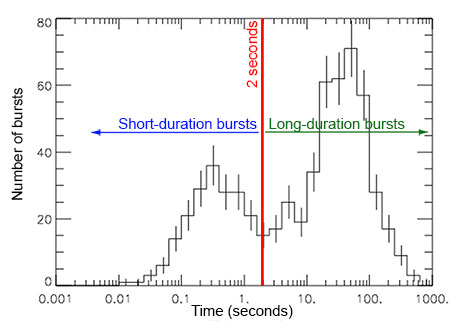
\includegraphics[width=0.5\textwidth]{Figuras/burst_durations_labelled.jpg}
  \caption{Gráfico que muestra la diferencia de tiempo que existe entre GRBs cortos y GRBs largos. Se pueden apreciar 2 picos que marcan la diferencia de duracion entre los GRBs}
  \label{fig:Batse_duration_GRBs}
\end{figure}

El objetivo principal del estudio de los GRBs es analizar las propiedades de los estallidos de los rayos gamma, así como sus progenitores y determinar las propiedades básicas de estos, la fusión de objetos compactos es el modelo progenitor más atractivo.
Las categorias de los GRBs largos y cortos son aproximadamente 75\% y 25\% de la población \cite{GRB:PPP}. %Gamma Ray Burst Progress, problems and prospects Zhang, meszaros
La interacción de flujos de salida relativistas con el medio ambiente que lo rodea produce emisión sincrotrónica que va desde la banda de las ondas de radio a los rayos X, los GRBs son uno de los eventos que más libera energía en el universo \cite{Berger:2013jza}, la energía liberada es del orden de $10^{52}$ ergs.

Aunque hay mucha información acerca de los GRBs largos, los cortos son aún un estudio nuevo en el área de astrofísica de altas energías ya que debido a su corta duración son difíciles de estudiar. 
\section{Características de los GRBs}
Muchas de las características de los GRBS ya sean estos largos o cortos, son la duración media que tienen, mientras que en los GRBs largos tienen un promedio de duración de 100 s \cite{PGRB-piran}, los GRBs cortos duran menos de 2 segundos. Los estallidos de Rayos gamma se encuentran a miles de años luz de nuestra galaxia por lo que se puede decir que tienen un orígen cosmologico, mientras los GRBs largos se originan en los centros de las galaxias, los cortos lo hacen lejos de la galaxia donde se originaron y por consecuencia, estos tienen una densidad de ambiente muy bajo. El estudio de los SGRB ha sido muy difícil debido al tiempo de duración que conllevan estos eventos y a la dificultad de asociarlo con galaxias anfitrionas. 

%Las partes principales de los GRBs son la emisión propmt y  afterglow. %Piran2005

\begin{figure} %fuente de la imagen:https://astrobites.org/2017/11/13/grb-afterglows-coming-out-of-a-cocoon/
  \centering
    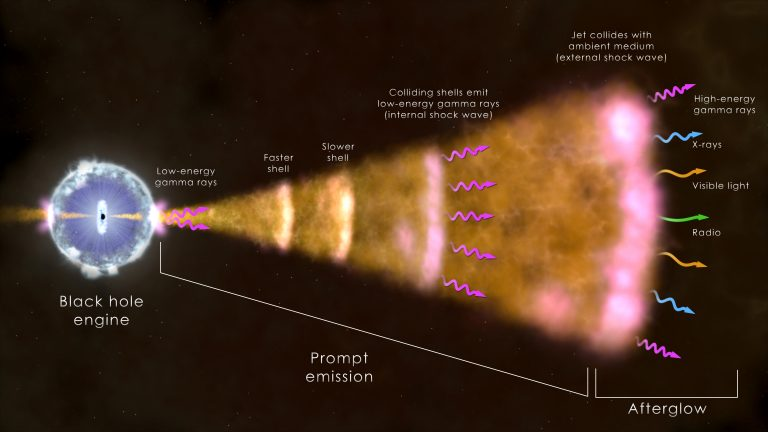
\includegraphics[width=0.5\textwidth]{Figuras/Gamma-ray_burst_by_a_blackhole-768x432.jpg}
  \caption{Diferentes partes de un GRB en general, mostrando las partes más características como el afterflow y la emisión prompt}
  \label{fig:Partes de GRBs}
\end{figure}
 

\subsection{Emisión pronta} %Azzam
La emisión pronta es definido como el periodo de tiempo donde el detector de rayos $\gamma$ detecta una señal sobre el fondo. Estas consisten en fotones de alta energía, no tiene espectro térmico \cite{GRB:CAP}. El espectro térmico es producido por un gas en equilibio térmico. Además, tiene bastantes carterísticas observacionales.

El flujo de energía varia dentro de cientos de Kev. La emisión de las curvas de luz son notoriamente irregulares sobre escalas de tiempo muy pequeñas \cite{SGRBr-Avanzo}(ver Figura \ref{lightcurve}). %Short gamma-ray bursts: A review; P. D’Avanzo
En los GRBs cortos, su espectro de emisión, se ha encontrado más duro que en los GRBs largos, esto debido a que es una combinación de componentes espectrales duros de baja energía. Una característica de principal es la duración de esta emisión, esta llega a ser del orden $\geq \, 10^{-2} $ s a $10^{3}$ s \cite{GRB:PPP}. Los valores promedio de dichas emisiones son $t \sim 20 $ s para GRBs largos y $t \sim 0.2 $ s para los cortos \cite{GRB:PPP}. %Gamma Ray Burst Progress, problems and prospects Zhang, meszaros

\begin{figure}
\centering %Fuente Zhang
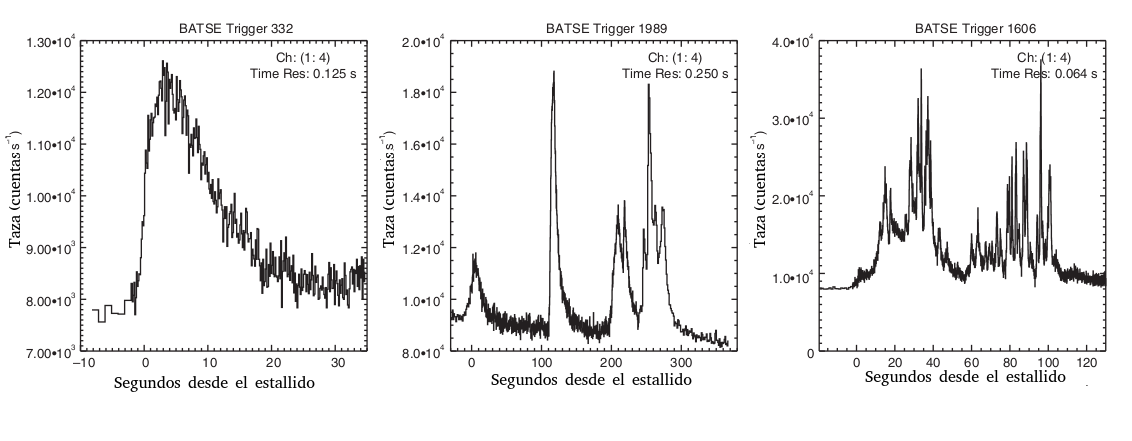
\includegraphics[width=1.0\textwidth]{Figuras/lightcurve_different}
\caption{\label{lightcurve} Diferentes curvas de luz captadas por el detector Batse detectadas en la emisión pronta de los GRBs. Las curvas de luz difieren bastantes unas de otras, mientras que BATSE 332 es un decaimiento exponencial , BATSE Trigger 1989  tiene 2 picos de intensidad. }
\end{figure}
\subsection{Emisión tardía}
La emisión tardía,conocida tambien como \emph{afterglow},  es después de la emisión prompt en el cual se pueden detectar otras longitudes de onda como el óptico, radio y los rayos X \cite{Berger:2013jza, PGRB-piran, SGRBr-Avanzo}. %\ref{fig:Partes de GRBs}.
La propiedad de "multiples longitudes de onda", hace una propiedad única de la emisión tardía. Estos cubren un amplio rango de frecuencias, desde las ondas de radio hasta los Tev. El espectro de banda ancha es descrito como una ley de potencias inversa, ya que la fuerza del choque se reduce a medida que la onda expansiva va desacelerando. Con lo que se espera que todas las longitudes de onda de las curvas de luz decaigan como ley de potencias. Entonces la densidad de flujo es proporcional a:

\begin{equation}
F_{\nu}(t,\nu) \propto t^{-\alpha} \nu^{\beta}
\end{equation}

Donde $\alpha$ y $\beta$ son reales positivos.


En Mayo y Julio del 2005 datos de eyecciones recopiladas por el satélite \emph{swift} al seguir al seguir al GRB 050509B, descubrieron las primeras fases tardías de los GRBs cortos, tiempo después el satélite HETE-2 junto con el observatorio \emph{chandra} de rayos X siguieron al satélite 050709 el cual localizo la fase tardía en rayos X y despues en la banda óptica, con estos datos recabados de la fase tardía se pudo llegar a que los GRBs cortos tienen una escala de densidad y una energía mas baja que los GRBs largos, tambien se llego a la conclusión de que los GRBs cortos tienen orígenes cosmologicos \cite{Berger:2013jza} y que las estrellas masivas no son sus progenitores como en el caso de GRBs cortos.
 
\subsection{Energía y luminosidad}
Los GRBs largos tienen una luminosidad isotrópica $L_{iso} \sim 10^{49}-10^{54} \, \mathrm{ergs} \cdot \mathrm{s}^{-1}$. También  hay GRBs largos con una luminosidad baja, sus valores rondan acerca de $L_{iso} \sim 5 \times 10^{46}-10^{49} \, \mathrm{ergs} \cdot \mathrm{s}^{-1}$, pero estos son solo una pequeña fracción de los GRBs largos observados. Los GRBs cortos tiene generalmente una luminosidad de $L_{iso} \sim 10^{49} \, \mathrm{ergs} \cdot \mathrm{s}^{-1}$.

La distribución de energías es amplia para los GRBs, estos cubren valores $E_{iso} \sim 10^{49}-10^{55}$ ergs para los largos y para los cortos $E_{iso} \sim 3.3 \times 10^{46}-10^{53}$ ergs \cite{Zhang:PGRB}. %the physics of gamma ray burst

%
\section{Características de los GRBs cortos}
Los GRBS cortos, aunque tiene muchas carcteristicas en común con los GRBs largos, también tienen sus propias peculariedades que lo hacen diferente del otro.

\subsection{Progenitores} %ghrels2009
Los GRBs cortos por lo general se localizan en medios de baja formación estelar por lo que no se espera poder encontrarlos ambientes estelares jovenes además de que, conllevan una carencia para poder asociarlos con SNs. El modelo más aceptado en la literatura de los progenitores de los GRBs cortos son la fusión de objetos compactos binarios. Estos pueden comprender a dos estrellas de neutrones (NS-NS), una estrella de neutrones y un agujero negro (NS-BH) o dos agujeros negros (BH-BH) \cite{GRB-SE}. La fusión se logra a cabo debido a la pérdida de momento angular y energía debido a las ondas gravitacionales. La interacción de este fenómeno lleva a la extracción de energía por procesos magnetohidrodinámicos (MHD), los cuales impulsan un flujo relativista colimado. 

Las patadas natales pueden ser las causantes de las distancias en las que estos nacen y los sitios de explosión de estos sistemas \cite{Berger:2013jza}, la probabilidad para una galaxia de brillo $m$  a ser localizada a una separación $\delta R$ de la posición de un SGRB está dada por 

\begin{equation}
P_{cc} = 1 - \exp ^{- \pi (\delta R)^{2} \sum(\leq m)}
\end{equation}
Donde $\sum(\leq m) = 1.3\cdot 10^{0.33(m-24)-2.44} \mathrm{arcsec} ^{-2}$ son el número de cuentas de la galaxia. Los SGRBs sin galaxias anfitrionas se exhiben cerca galaxias de campo con una baja probabilidad de coincidencia, generalmente las distancias medias de separación del SGRB con su galaxia anfitriona es de $ \frac{\delta R}{r_e} \approx 1.5$ donde $r_e$ es el radio estelar. 

\subsection{Propiedades de las explosiones de los SGRB}

Los parámetros claves de interés de la emisión pronta y tardia \cite{Berger:2013jza}
\begin{itemize}
\item $E_{\gamma}$: Energía de rayos $\gamma$.
\item $E_k$: Energía cinética de la onda de choque de la emisión tardía.
\item $\theta_j$: El ángulo de apertura del jet.
\item $n$: Densidad del medio ambiente.
\end{itemize}

La emisión del sincrotrón de la emisión tardía incluye dos parámetros libres que tienen relación con la física del choque relativista:
\begin{itemize}
\item $\epsilon_{B}$: Fracción de energía del post-choque de los campos magnéticos.
\item $\epsilon_e$: Radiación relativista de los electrones. 
\end{itemize}



El flujo relativista interactuando con el medio circundante es el espectro de emisión sincrotónico. Esta se caracteríza por 3 frecuencias de corte:
\begin{itemize}
\item $\nu_a$: Auto absorción
\item $\nu_m$: Factor mínimo de Lorentz
\item $\nu_c$: enfriamiento sincrotrónico
\end{itemize}

Tomando en cuenta los valores de estos parámetros y la pendiente del espectro para $\nu < \nu_m$ se pueden llegar a encontrar los siguientes valores $E_{k, \, \mathrm{iso}}$, $n$, $\epsilon_{B}$ y $\epsilon_e$. La evolución temporal del espectro también se puede usar para encontrar el ángulo de apertura del jet $\theta_j$. La relacción que existe entre el ángulo de apertura $\theta_j$ y el tiempo $(t_j)$ al cual ocurre el jet break  está dado por la siguiente fórmula.

%La mayoría de estas frecuencias se encuentran entre 1 $\thicksim$ 10 GHz por lo cual ha sido difícil de detectarlas. La colimación del jet también influye en la taza de los SGRBs y proporciona una restricción adicional al modelo progenitor, la firmatura de la colimación de los destellos de los SGRBs son los llamados "Jet Break" que ocurren al tiempo $t_j$ cuando $\Gamma_j(t_j) = 1/ \theta_j$, esto lidera al cambio de emisión del espectro sincrotrónico
%
%\begin{equation}
%F_\nu \propto t^{-1} \longrightarrow F_\nu \propto t^{-p}
%\end{equation}
%
%La relación entre el "jet break" y el ángulo de apertura esta dado por:
%
\begin{equation}
\theta_j = 0.13 \left( \frac{t_{j,d}}{1+z} \right)^{3/8}
\left(\frac{n_0}{E_{52}} \right)^{1/8}
\end{equation}
%
%\section{GRB del 17 de agosto del 2017}
%

\begin{figure}
\centering
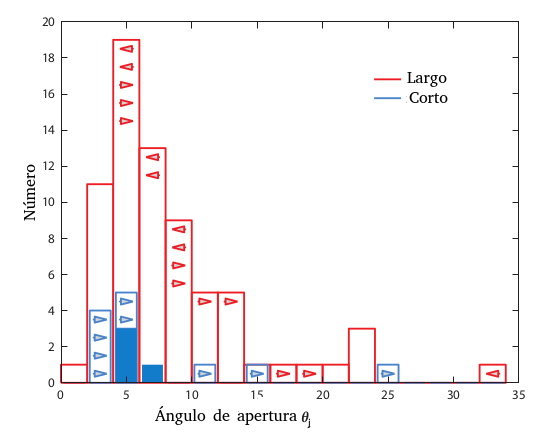
\includegraphics[scale=0.7]{./Figuras/Distribucion_angulo_apertura}
\caption{La Figura muestra la distribución de los ángulos de apertura para los GRBs largos (rojos) y los GRBs cortos (azules). Las flechas muestran el límite superior e inferior de los ángulos. }
\end{figure}

\chapter{Teoría}

Los GRBs, ya sean largos o cortos, que se originan en el medio interestelar, se pueden describir como un fluido sin viscosidad y estos pueden ser descritos bajo
las ecuaciones de la hidrodinámica.
Para describir un sistema de partículas como un fluido bajo ciertas condiciones uno debe de conocer que el camino libre medio debe de ser mucho mas pequeño que la escala de longitud de las fluctuaciones de las variables macroscópicas.

\begin{equation}
\lambda_{mfp} \ll L
\end{equation}

El tiempo entre las colisiones debe de ser pequeña comparada con la escala del tiempo de los cambios en el fluido
\begin{equation}
t_{c} \ll t_f
\end{equation}
La distancia media entre las partículas tiene que ser mas pequeña que la longitud de escala de las variables macroscópicas

\begin{equation}
l = n^{-1/3} \ll L
\end{equation}



\section{Ecuaciones de la hidrodinámica}


Considerando una serie de elementos de volumen fijos, las ecuaciones que describen el movimiento de un fluido sin considerar efectos viscosos son:

La conservación de masa
\begin{equation} \label{conservación_masa_hidrodinamica}
\dfrac{\partial \rho }{\partial t} + \nabla \cdot \left( \rho \mathbf{u} \right)
\end{equation}

El momento
\begin{equation}  \label{conservacion_momento_hidrodinamica}
\dfrac{\partial \left( \rho \mathbf{u} \right) }{\partial t}+ \nabla \cdot \left( \rho \mathbf{u u} \right) + \nabla p = \mathbf{f_{ext}}
\end{equation}

Ecuación de la energía

\begin{equation} \label{conservacion_energia_hidrodinamica}
\dfrac{\partial E }{\partial t} + \nabla \cdot \left[ \mathbf{u} \left( e+p \right) \right] =G-L+\mathbf{f_{ext} \cdot \mathbf{u}}
\end{equation}

Ecuación de estado
\begin{equation}
e=\frac{1}{2} \rho \mathbf{u}^{2} + \frac{p}{\Gamma - 1}
\end{equation}

Con estas ecuaciones podemos formar una matriz de $5x5$ escritas en coordenadas cartesianas:

\begin{equation} \label{euler_cartesianas}
\dfrac{\partial \mathbf{U}}{\partial t}+\dfrac{\partial \mathbf{F}}{\partial x}+\dfrac{\partial \mathbf{G}}{\partial y}+\dfrac{\partial \mathbf{H}}{\partial z}= \mathbf{S}
\end{equation}

Donde
\begin{center}


$\mathbf{U}=
\left(\begin{smallmatrix}
\rho \\
\rho u \\
\rho v \\
\rho w \\
E \\
\end{smallmatrix}\right)
$,
$\mathbf{F} =
\left(\begin{smallmatrix}
\rho u \\
\rho u^{2}+P \\
\rho uv \\
\rho uw \\
u(e+P) \\
\end{smallmatrix}\right)
$,
$\mathbf{G} =
\left(\begin{smallmatrix}
\rho v\\
\rho vu \\
\rho v^{2}+P \\
\rho vw \\
v(e+P) \\
\end{smallmatrix}\right)
$,
$\mathbf{H} =
\left(\begin{smallmatrix}
\rho w\\
\rho wu \\
\rho wv \\
\rho w^{2}+P \\
w(e+P) \\
\end{smallmatrix}\right)
$, 
$\mathbf{S} =
\left(\begin{smallmatrix}
0 \\
f_{x} \\
f_{y} \\
f_{z} \\
G-L+\textbf{f} \cdot \textbf{u} \\
\end{smallmatrix}\right)
$
\end{center}

El término de $\mathbf{U}$ son nuestras variables conservadas, los términos $\mathbf{F}$, $\mathbf{G}$, $\mathbf{H}$ son nuestros fluidos  con velocidades en la dirección $x$, $y$ y $z$ y $\mathbf{S}$ son los términos fuente. Para poder resolver computacionalmente estas ecuaciones diferenciales parciales vamos a utilizar el método de las diferencias finitas y el método de Lax sin considerar tos términos fuente es decir $\mathbf{S}=0$ en el siguiente capitulo si se trataran fuentes particulares.

La implementación en el código se hará en 2 dimensiones por lo que la variable \emph{H} que corresponde a los flujos en el eje z será cero el bloque de código esta en una subrutina llamada \emph{fluxes}, 
donde en el mismo bucle se desacoplan las primitivas para que queden en función de las conservadas.Cabe señalar que tanto en $f(4,i,j)$ y $g(4,i,j)$ se usa la
la variable conservada $u(4,i,j)$, ya que $u(4,i,j) = e$ . 


\begin{lstlisting}[frame=single]

  f(1,i,j)=rho*vx
  f(2,i,j)=rho*vx*vx+P
  f(3,i,j)=rho*vx*vy
  f(4,i,j)=vx*(u(4,i,j)+P)

  g(1,i,j)=rho*vy
  g(2,i,j)=rho*vx*vy
  g(3,i,j)=rho*vy*vy+P
  g(4,i,j)=vy*(u(4,i,j)+P)

\end{lstlisting}

Las variables \emph{i}, \emph{j} corren sobre todo el dominio espacial dentro de un bucle, el término $\mathbf{H}$ no es incluido, debido a que es computacionalmente 
caro. El término \emph{u} hace alusión a las variables conservadas.

\subsection{Desacoplamiento de las ecuaciones de la hidrodinámica}

Al final del metodo de las diferencias finitas, obtenemos nuestras variables conservadas (\emph{U}), pero para calcular nuestros flujos de nuevo necesitamos recuperar nuestras primitas, es decir, calcular nuestras variables primitivas $(\rho, \, u, \, v,\, w, \, P )$ en función de nuestras variables conservadas $(u_1, \, u_2, \, u_3, \, u_4, \, u_5)$.

Despejar la densidad es sencillo ya que es directo $u_1= \rho$ por lo tanto:

\begin{equation}\label{primitiva_densidad}
\rho = u_1
\end{equation}

Para las velocidades $u_i=\rho \upsilon$, donde $i=2,3,4$ y $\upsilon=u,v,w$, nos da $\upsilon= u_i/ \rho$ y usando la ecuación \ref{primitiva_densidad} queda:

\begin{equation} \label{primitiva_velocidades}
\upsilon = u_1/u_i
\end{equation}
Para la ecuacion de la energía $u_5=E$ combinando con la ecuacion de estado y la ecuación \ref{primitiva_velocidades} obtenemos
\begin{equation}
P = \left( \Gamma - 1 \right) \left[ u_5 - \frac{u_1 \left( \sum_{i=2}^{4} u_1/u_i \right)^2}{2} \right]
\end{equation}

En el código se implenta de la siguiente manera.
Las variables \emph{i}, \emph{j} son contadores, y antes de que se calculen los flujos, se tienen que calcular las primitivas. Dado que el desacoplamiento
se implementa directamente en la subrutina \emph{fluxes}, para que se puedan calcular los flujos.

\begin{lstlisting}[frame=single] 
  

    !Desacoplamiento de las primitivas
    rho = u (1,i,j)
    vx  = u(2,i,j)/rho
    vy  = u(3,i,j)/rho
    P   = (u(4,i,j)-0.5*rho*(vx**2+vy**2))*(gamma-1.)

\end{lstlisting}

Racordemos que la variable \emph{u(4,i,j)} es la energía.
  


\section{Hidrodinámica relativista}
Los GRBs generalmente tienen velocidades relativistas, por lo que la parte newtoniana no nos va a servir, pero si nos servira como apoyo para poder pasar
a la hidrodinámica relativista.
En esta parte se añadirá a los códigos que ya hemos generado previamente, las próximas secciones abordara acerca de como cambian nuestras primitivas,
como afectan a nuestras variables conservadas y como las podemos desacoplar así como varios ejemplos al cambiar varios valores de nuestros parámetros y 
de las condiciones iniciales.

\subsection{Primitivas}
Las ecuaciones que teníamos para fluidos newtonianos se pueden modificar para hacerlos relativistas. Para esto vamos a partir de 2 ecuaciones importantes que son la ecuación de energía-momento y la ecuación de conservacion de masa:

\begin{equation}\label{Ecuacion_conservación_masa}
\left( \rho u^{\alpha} \right)_{, \alpha} =0
\end{equation}

\begin{equation}\label{Ecuacion_momento_energia}
T_{, \beta}^{\alpha \beta}=0
\end{equation}

De la ecuación \ref{Ecuacion_conservación_masa} tenemos la cuadrivelocidad para un sistema de 3 coordenadas y considaremos a la velocidad de la luz como $c=1$ lo podemos ver como $u^{\mu}=\gamma \left( 1, \textbf{v}\right)$ y sustituyendo este resultado (en 2 dimensiones espaciales) tendremos las ecuaciones $u_1$, $F_1$ y $G_1$. Para la ecuación \ref{Ecuacion_momento_energia} podemos escribir el tensor de energía-momento como $T^{\mu \nu} = \rho h u^{\mu} u^{\nu} + Pg^{\mu \nu}$ y usando la métrica de Minkowski

\begin{equation}
\eta_{\alpha \beta}= 
\begin{pmatrix}
 -1 & 0 & 0 & 0 \\
 0 & -1 & 0 & 0 \\
 0 & 0 & -1 & 0 \\
 0 & 0 & 0 & 1 \\
\end{pmatrix}
\end{equation}

Con lo que podemos escribir a $T^{\mu \nu}$ matricialmente como:

\begin{equation}
T^{\mu \nu} =
\begin{pmatrix}
\rho h \gamma^2-P & \rho h \gamma^2 v_{x}  & \rho h \gamma^2 v_{y} & \rho h \gamma^2 v_{z} \\

\rho h \gamma^2 v_{x} & \rho h \gamma^2 v_{x}^{2}+P & \rho h \gamma^2 v_{x}v_{y} &  \rho h \gamma^2 v_{x}v_{z} \\

rho h \gamma^2 v_{y} & \rho h \gamma^2 v_{y}v_{x} & \rho h \gamma^2 v_{y}^{2}+P & \rho h \gamma^2 v_{y}v_{z}\\

\rho h \gamma^2 v_{z} & \rho h \gamma^2 v_{z}v_{x} & \rho h \gamma^2 v_{z}v_{y} & \rho h \gamma^2 v_{z}^2 + P

\end{pmatrix}
\end{equation}
Entonces nuestras ecuaciones quedarían de la siguiente manera
\begin{align}
u_{1}& = \rho \gamma \\ 
u_{2}& = \rho v_{x} \gamma^{2} h \\ 
u_{3}& = \rho v_{y} \gamma^{2} h \\ 
u_{4}& = \rho \gamma^{2} h - P 
\end{align}

Donde $\rho$ es la densidad, $\gamma$ es el factor de lorentz, $v_{x}$ y $v_{y}$ son las velocidades de nuestros fluidos (en 2 dimensiones pero se puede extender esto a 3 sin ningún problema), $h$ es la entalpía  y $P$ es la presión. Para los fluidos quedan de la siguiente manera
\begin{align}
F_{1}& = \rho v_{x} \gamma \\ 
F_{2}& = \rho v_{x} v_{x} \gamma^{2} h + P\\ 
F_{3}& = \rho v_{x} v_{y} \gamma^{2} h \\ 
F_{4}& = \rho v_{x} \gamma^{2} h 
\end{align}

\begin{align}
G_{1}& = \rho v_{y} \gamma \\ 
G_{2}& = \rho v_{y} v_{x} \gamma^{2} h \\ 
G_{3}& = \rho v_{y} v_{y} \gamma^{2} h + P\\ 
G_{4}& = \rho v_{y} \gamma^{2} h
\end{align}
\begin{align}
H_{1}& = \rho v_{z} \gamma \\ 
H_{2}& = \rho v_{z} v_{x} \gamma^{2} h \\ 
H_{3}& = \rho v_{z} v_{y} \gamma^{2} h \\ 
H_{4}& = \rho v_{z}^{2} \gamma^{2} h + P
\end{align}

La implementación en el código es de la siguiente manera, el factor de Lorentz $\gamma$ es la variable lor, $h$ la entalpía, al igual que en la hidrodinámica
newtoniana solo se considerará 2 dimensiones:

\begin{lstlisting}[frame=single]
  lor=1/sqrt(1-(vx**2+vy**2))
  h=1.+gamma/(gamma-1.)*P/rho
  
  f(1,i,j)=rho*vx*lor
  f(2,i,j)=rho*vx*vx*lor**2*h+P
  f(3,i,j)=rho*vx*vy*lor**2*h
  f(4,i,j)=rho*vx*lor**2*h

  g(1,i,j)=rho*vy*lor
  g(2,i,j)=rho*vx*vy*lor**2*h
  g(3,i,j)=rho*vy*vy*lor**2*h+P
  g(4,i,j)=rho*vy*lor**2*h

\end{lstlisting}

A diferencia de los flujos newtonianos, para los flujos relativistas se tienen que calcular antes el factor de Lorentz \emph{lor} y la entalpía \emph{h},
las variables \emph{i}, \emph{j} son contadores sobre el espacio.

\subsection{Desacoplamiento de las ecuaciones de la hidrodinámica relativista} \label{Cap_Desacoplamiento_de_las_ecuaciones_de_la_hidrodinámica_relativista}
Para poder desacoplar las ecuaciones, partimos de la relación de las densidades de energía total y del módulo de los momentos

\begin{equation}\label{ecuacion_de_energia}
e=W-p
\end{equation}

\begin{equation}\label{modulos de los momentos}
\abs{m}^2= W^{2}\abs{v}^{2}
\end{equation}

Donde $W=D h \gamma$ y $D=\rho \gamma$. Para evitar errores en el límite no relativista se debe resolver la ecuación conservada restando la densidad de masa 
a la energía para definir una nueva variable conservada ($e^{'}=e-D$), para las cancelaciones en el límite ultra-relativista basados en $\gamma \abs{v^2}$ que se tiene cuando $\abs{v} \rightarrow 1$, se debe de crear otra variable, que en este caso seria $\abs{u}^2=\gamma \abs{v^2}$ e introduciendo las variables $W^{'}=W-D$. Podemos re-escribir la última ecuación de la siguiente manera

\begin{eqnarray*}
 W^{'}& = &D(h \gamma -1)\\
&=& D\left[ \left(1-\epsilon+ \frac{p}{\rho}\right) \gamma - 1 \right]\\
&=& D \left(\gamma-1 \right) \frac{\gamma+1}{\gamma+1}+\frac{D \gamma }{\rho}\left(\rho \epsilon + p \right)
\end{eqnarray*}

Recordando que $D=\rho \gamma$ y que a partir de la variable introducida $u^{2}$ podemos re-scribir el factor de Lorentz como $\gamma^{2} = 1- u^{2}$

\begin{eqnarray}\label{W_prima}
\nonumber W^{'}&=&\frac{D u^{2}}{\gamma + 1}
+\frac{\rho\gamma \gamma}{ \rho }\left(\rho \epsilon + p \right)\\
&=& \frac{D u^{2}}{\gamma + 1} + \gamma^{2} \chi
\end{eqnarray}

Donde $\chi=\rho \epsilon + p$, derivando con respecto a $W^{'}$ la ecuación \ref{ecuacion_de_energia} queda como
\begin{equation}\label{derivada_E_W}
\dfrac{de}{dW^{'}}=1-\dfrac{dp}{dW^{'}}
\end{equation}

Nosotros no sabemos como es la expresión $\dfrac{de}{dW^{'}}$, así que asumiremos que $p=p(\rho, \chi)$ por lo que podemos aplicar la regla de la cadena (para mas detalles consulte)
\begin{equation}\label{cadena}
\dfrac{dp}{dW^{'}}=\dfrac{\partial p}{\partial\chi}\Bigg |_{\rho} \dfrac{d\chi}{dW^{'}} + \dfrac{\partial p}{\partial \rho}\Big |_{\chi} \dfrac{d \rho}{d W^{'}}
\end{equation}

Para calcular $\dfrac{dp}{d\chi}$ tenemos que por ser el caso de un gas ideal
\begin{equation} \label{entalpia_funcion_presion_densidad}
h=1+\frac{\Gamma}{\Gamma-1}\frac{p}{\rho}
\end{equation}
Donde $h$ también puede ser escrito como
\begin{equation}
h=1+\epsilon+\frac{p}{\rho}
\end{equation}
Si combinamos estas 2 últimas ecuaciones podemos llegar a que 
\begin{equation}
p(\chi,\rho)=\frac{\Gamma-1}{\Gamma}\chi
\end{equation}

Con lo que al derivar con respecto de $\chi$ nos da como resultado
\begin{eqnarray}\label{der_presion}
& \dfrac{d p}{d \chi}&=\frac{\Gamma-1}{\Gamma}\\ &\dfrac{d p}{d \rho}&= 0
\end{eqnarray}

De la ecuación \ref{W_prima} podemos despejar $\chi$, lo que queda como
\begin{equation}
\chi=\frac{W^{'}}{\gamma}- \frac{D u^{2}}{(1+\gamma)\gamma^{2}}
\end{equation}

Derivando implícitamente la ecuación \ref{W_prima} respecto a $W^{'}$ nos quedaría
\begin{eqnarray*}
W^{'}&=&D\left(\gamma-1 \right) + \chi \gamma^{2}\\%saloto de linea
&=& D\left(\frac{1}{\sqrt{1-\nu^{2}}} -1\right)+\chi \dfrac{1}{1-\nu^{2}} \\%saloto de linea
\dfrac{d W^{'}}{d W^{'}} &=& D \dfrac{d (1-v^2)^{-1/2}}{d W^{'}}+\dfrac{d \chi}{dW^{'}}(1-v^2)^{-1}+\dfrac{d (1-v^2)^{-1} }{d W^{'}}\chi \\  %salto de linea 
1 &=& \frac{D(1-v^2)^{-3/2}}{2} \dfrac{d v^{2}}{d W^{'}}+\dfrac{d \chi}{dW^{'}}(1-v^2)^{-1}+ \chi (1-v^2)^{-2}  \dfrac{d v^{2}}{d W^{'}} \\ %salto de linea
\frac{1}{\gamma ^2} &=& \frac{D \gamma}{2} \dfrac{d v^{2}}{d W^{'}} + \dfrac{d \chi}{dW^{'}} + \chi \gamma^2 \dfrac{d v^2}{dW^{'}} \\ %salto de linea
\end{eqnarray*}

Con lo que al final la ecuación se puede escribir de la siguiente manera

\begin{equation}\label{der_chi}
\dfrac{d \chi}{dW^{'}}=\frac{1}{\gamma^2}-\frac{\gamma}{2}(D-2\gamma \chi) \dfrac{d v^2}{dW^{'}}
\end{equation}

Y para

\begin{equation}\label{der_rho}
\dfrac{d \rho}{d W^{'}}= D \dfrac{d\left(1/ \rho \right) }{d W^{'}} = - \frac{D \gamma}{2}  \dfrac{d v^2}{dW^{'}}
\end{equation}

despejando la ecuación \ref{modulos de los momentos} podemos llegar a escribir el módulo de la velocidad al cuadrado de la siguiente manera
\begin{equation}
\abs{v^{2}} = \frac{\abs{m^{2}}}{W^{'}} 
\end{equation}
Donde $m_i= \rho v_i \gamma h$ para $i=x,y$.

Podemos demostrar que $\dfrac{d \abs{v^2}}{W}=\dfrac{d \abs{v^2}}{W^{'}}$ para esto vamos a partir de de lo siguiente 
\begin{eqnarray*}
\abs{v^2}&=& \abs{m^{2}} \left(W^{'} + D \right)^{-2} \\
\dfrac{d \abs{v^2}}{d W^{'}} &=& \frac{-2 \abs{m}^2}{W^{'}+D^{3}} \\
&=& \frac{2 \abs{m}^2}{W^{3}} \\
&=& \dfrac{d \abs{v^2}}{d W^{'}}
\end{eqnarray*}

Con lo que podemos decir que 

\begin{equation}\label{der_v2}
\dfrac{d\abs{v}^2}{d W^{'} }=-\frac{2 \abs{m}^{2}}{W^{3}}
\end{equation}
Con todo esto ya sabemos cuanto es lo que vale la ecuación \ref{derivada_E_W}, con esto ya podemos usar el método de Newton-Raphson para poder encontrar $W^{'}$.\\

El método de Newton-Raphson es un algoritmo iterativo que se usa para encontrar raíces  de una función real:

\begin{equation} \label{eq_Newton_Raphson}
W^{'(k+1)}=W^{'}-\frac{f(W^{'})}{\dfrac{d f(W^{'})}{d W^{'}}}
\end{equation}

De la ecuación de la densidad de energía, podemos utilizarla como a la función a la que queremos encontrar la raíz

\begin{equation} \label{ecuación_f}
f(W^{'})=W^{'}-e^{'}-p
\end{equation}

Donde $e^{'}=W^{'}-p$ y que $\dfrac{d f(W^{'})}{d w} \equiv \dfrac{de}{dW^{'}}$ dado por la ecuación \ref{derivada_E_W}. 
Para iniciar el proceso de iteración se tiene que hacer una suposición, para esto, con ayuda de las ecuaciones \ref{ecuacion_de_energia} 
y \ref{modulos de los momentos} podemos llegar a que la presión es:
%===============================================================================================

\begin{equation} \label{presion_de_newton}
p=\frac{\abs{m}^{2}-W^{2}\abs{v}^{2}+4W^{2}-4EW}{4W}
\end{equation}

Como podemos ver el denominador es una función convexa cuadrática que depende $\abs{v}^{2}$ y $W$ y cumple con que $W$ este fuera del intervalo de las raíces positivas y negativas.

Al denominador de la  ecuación podemos encontrar $W$ ya que $\abs{v}^{2}=1-1/\gamma^{2}$ suponiendo $\gamma \rightarrow \infty$ podemos despejar $W$

\begin{equation}\label{suposicion_de_W}
W=\frac{-(-2E)+\sqrt{(-2E)^{2}-(3)(\abs{m}^{2})}}{3}
\end{equation}

Con esto ya se puede hacer las aproximaciones para obtener $W$, y podemos calcular las siguientes relaciones 
\begin{eqnarray}
\abs{v}^{2} &=& \frac{\abs{m}^{2}}{W^{2}}\label{prim_v2}\\ 
u^{2}&=&\frac{\abs{v}^{2}}{1-\abs{v}^{2}}\label{u2}\\
\gamma &=& \sqrt{1+u^{2}}
\end{eqnarray}
Y las nuevas primitivas.\\

Velocidades:
\begin{eqnarray}
v_{x}&=&\frac{u_{2}}{W}\\
v_{y}&=&\frac{u_{3}}{W}\\
\end{eqnarray}

Densidad de masa 
\begin{equation}
\rho=\frac{D}{\gamma}
\end{equation}

Presión térmica
\begin{eqnarray}
\chi&=&\frac{W-D}{\gamma^{2}}-\frac{D \abs{u}^{2}}{(1+\gamma)\gamma^{2}}\\
p&=&\frac{\Gamma-1}{\Gamma} \chi
\end{eqnarray}

Aunque en el método newtoniano se podian desacoplar las ecuaciones sobre el mismo bucle, 
para el método relativista se tuvo que crear una subrutina para poder desacoplar las primitivas y asi poder obtenerlas en funcion de las conservadas. 
Al igual que en el método newtoniano vamos a correr el bucle sobre nuestra malla. La subrutina de desacoplamiento se llama \emph{uprim}, 
y esta recibe un parámetro de entrada, que es la conservada \emph{u} y nos devuelve una variable primitiva. 
Las variables conservadas las reasignmos a unas nuevas llamadas \emph{qu} para que podamos usar la subrutina, una vez que se desacoplan, 
los valores de salida los reasignamos a otras llamadas \emph{qpp}. Se tienen que reasignar dado que la subrutina pide números reales y no matrices.

\begin{lstlisting}[frame=single] 
        
    qu(1) = u(1,i,j)
    qu(2) = u(2,i,j)
    qu(3) = u(3,i,j)
    qu(4) = u(4,i,j)

    ! Desacoplamiento de las primitivas
    call uprim(u,qp)

    qpp(:,i,j)=qp

    rho = qpp(1, i,j)
    vx  = qpp(2, i,j)
    vy  = qpp(3, i,j)
    P   = qpp(4, i,j)


\end{lstlisting}

La subrutina de desacoplamiento para las variables conservadas que se mencionan en esta sección recibirá las variables conservadas
y devolverá las primitivas. La subrutina \emph{newrap} se usará en particular 
(ver apéndice \ref{ap_newrap}) para resolver la ecuación \ref{eq_Newton_Raphson}.

\begin{lstlisting} [frame=single]
  
  m2 = sum(qu(2:3)**2)               ! v^2

  call newrap(qu, w, m2)

  alpha = m2 / w**2   ! alpha < 1 !
  u2  = alpha/(1.0-alpha)

  lor = sqrt(1.0 + u2)

  ! velocities
  qp(2:3) = qu(2:3) / w

  ! determination of the mass density
  qp(1) = qu(1)/lor

  ! thermal pressure
  chi = (w - qu(1)*(1.0+u2/(lor+1.0)))/(1.0+u2)

  qp(4)   = (gamma - 1.0)/gamma * chi

  qp(4) =max(qp(4),1d-10*qp(1))
\end{lstlisting}

Las variables \emph{qp} mostradas en el código son las primitivas mientras que las otras son auxiliares mostradas en el capitulo 
\ref{Cap_Desacoplamiento_de_las_ecuaciones_de_la_hidrodinámica_relativista}


\section{Diferencias finitas} \label{sec:Diferencias_finitas}
Ya hemos visto que ecuaciones describen la hidrodinámica, ahora nos toca resolverlas, dado que analíticamente es difícil, se va a hacer computacionalmente, para 
eso se hará uso del método numérico de las diferencias finitas.
Si tenemos una función $f(x)$ lo suficientemente diferenciable la podemos aproximar por el Teorema de Taylor  en la vecindad de un punto $x_0+\Delta x$ entonces si conocemos todas sus $n$ derivadas de la función $f(x)$ en el punro $x_0$ podemos aproximar de la siguiente manera

\begin{equation}\label{Serie_Taylor}
f\left( x_0 + \Delta x\right) = f\left( x_0 \right)+
\sum_n \frac{\left( \Delta x \right) ^2}{k!}f^{(k)} \left(x_0
\right)
\end{equation}

Si truncamos la serie de Taylor y quitamos los términos de segundo orden podemos escribir la ecuación \ref{Serie_Taylor} como:

\begin{equation}
f\left( x_0 + \Delta x \right) = f(x_0) - \Delta x f^{(1)} (x_0) + O \left( \Delta x \right)
\end{equation}

Despejando $f(x_0)$ queda lo que se conoce como diferrencia finita hacia adelante
\begin{equation}\label{fwd}
f_{fwd}^{'}=\frac{f\left(x + \Delta x \right) - f(x) }{\Delta x}=\frac{f_{i+1}-f_{i}}{\Delta x}
\end{equation}

Tambien se puede hacer en el entorno $x_0- \Delta x$ y siguiendo los mismos pasos anteriores llegamos a lo que se le conoce como diferencia finita hacia atras.



\begin{equation}\label{bwd}
f_{back}^{'}=\frac{f\left(x \right) - f(x - \Delta x) }{\Delta x}=\frac{f_{i}-f_{i-1}}{\Delta x}
\end{equation}

Si obtenemos el promedio de las ecuaciones \ref{fwd} y \ref{bwd} obtenemos la central:

\begin{equation} \label{Centrada}
f_{central}^{'}=\frac{f\left(x + \Delta x\right) - f(x - \Delta x) }{2\Delta x}=\frac{f_{i+1}-f_{i-1}}{2 \Delta x}
\end{equation}



\subsection{Lax-Friederich}

Si consideramos la siguiente ecuación diferencial parcial

\begin{equation} \label{ecu_conser}
u_t+ f\left(u \right)_t=0
\end{equation}

Un método conservativo para resolver este tipo de ecuación diferencial es 

\begin{equation}\label{esquema conservativo}
u_i^{n+1} = u_i^{n} -\frac{\Delta t}{\Delta x} \left(f_{i-\frac{1}{2}} - f_{i+\frac{1}{2}}\right)
\end{equation}



Si hacemos la siguiente elección de flujo 

\begin{equation}
f_{i+\frac{1}{2}} = f_{i+\frac{1}{2}} \left(
u_{i} , u_{i+1}\right) =\frac{1}{2} \left(f_{i} + f_{i+1} \right) 
\end{equation}

Y para 

\begin{equation}
f_{i-\frac{1}{2}} = f_{i-\frac{1}{2}} \left(
u_{i} , u_{i-1}\right) =\frac{1}{2} \left(f_{i} - f_{i-1} \right) 
\end{equation}

Y lo sustituimos en la ecuación \ref{esquema conservativo} nos queda el siguiente resultado

\begin{equation}\label{ec_inestable}
u_i^{n+1} = u_i^{n} + \frac{1}{2}\frac{\Delta t}{\Delta x} \left(f_{i+1} - f_{i-1} \right)
\end{equation}

Pero esta solución es inestable, por el primer término del lado derecho de la ecuación, para hacerlo estable  Peter Lax y Kurt O. Friedrichs sustituyerón este término por $(u_{i+1}^n-u_{i-1}^n)$  por lo que podemos reescribir la ecuación \ref{ec_inestable} como

\begin{equation}\label{ec_estable}
u_i^{n+1} =(u_{i+1}^n-u_{i-1}^n) + \frac{1}{2}\frac{\Delta t}{\Delta x} \left(f_{i+1} - f_{i-1} \right)
\end{equation}

En el código, la implementación de la ecuación \ref{ec_estable} en 2 dimensiones es la siguiente

\begin{lstlisting} [frame=single]

  call fluxes(nx,ny,neq,gamma,u,f,g,bound)

  do i=1,nx
    do j=1,ny
      up(:,i,j)=0.25*( u(:,i-1,j)+u(:,i+1,j)+u(:,i,j-1)+u(:,i,j+1) ) &
                  -dtx*0.5*(f(:,i+1,j)-f(:,i-1,j) ) &
                  -dty*0.5*(g(:,i,j+1)-g(:,i,j-1) )
    end do
  end do
  
\end{lstlisting}

Donde \emph{dtx, dty} son las derivadas con respecto a \emph{x}, \emph{y} y \emph{up} es la conservada posterior en el tiempo.



\subsection{HLL}

	Otro método para resolver las ecuaciones de la hidrodinámica es usar el método de Harten-Van-Leer. Definiendo el flujo numérico intercelda de Gudonov

\begin{equation}
F_{i+\frac{1}{2}}=F \left( U_{i+\frac{1}{2}} \right)
\end{equation}

Para el cual $U_{i+\frac{1}{2}}(0)$ tiene la misma solución para $U_{i+\frac{1}{2}}(x/t)$ con lo que el problema de Riemann se reduce a :

\begin{equation} \label{Ecuacion_discreta_conservada}
\begin{array}{ll}
U_t + F \left( U \right)_x = 0 \\
U \left(x,0 \right) = 
\left\lbrace
\begin{array}{rr}
U_L \quad \textup{si} \quad x<0  \\
U_R \quad \textup{si} \quad x>0
\end{array}
\right.
\end{array}
\end{equation}

\begin{figure} %fuente de la imagen:libro del toro/
  \centering
    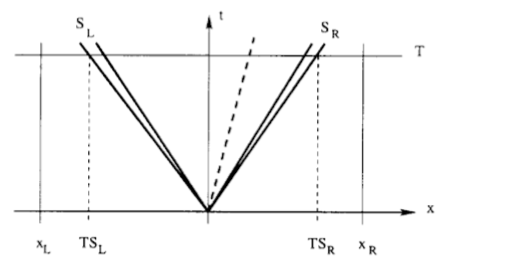
\includegraphics[width=0.5\textwidth]{Figuras/HLL_onda.png}
  \caption{Plano x-t que muestra que muestra un volumen definido}
  \label{fig:Plano x_t}
\end{figure}

Si consideramos un control de volumen $\left[x_L, x_R \right]\times \left[ 0 , T \right]$, tales que $x_L \leq TS_L$ y $x_R \geq TS_R$ (ver Figura \ref{fig:Plano x_t}) donde $S_L$ y $S_R$ son las velocidades de las ondas mas rápidas de los 
estados iniciales $U_L$ y $U_R$ respectivamente y $T$ es un tiempo definido. Si usamos la forma integral de la 
ecuacion \ref{Ecuacion_discreta_conservada} en nuestro volumen definido $\left[x_L, x_R \right]\times \left[ 0 , T \right]$

\begin{equation*}\label{Forma_integral_conservadas}
\int_{x_L}^{x_R} \left[ U\left( x, T \right) -
 U\left( x, 0 \right) \right] dx = 
 \int_{0}^{T} \left[ F \left(U\left( x_L, t \right) \right) -
 F \left(U\left( x_R, t \right) \right) \right] dt 
\end{equation*}
Entonces
\begin{equation}\label{integral_consistencia}
\int_{x_L}^{x_R} U\left( x, T \right) dx =\int_{x_L}^{x_R} U\left( x, 0 \right) dx+
\int_{0}^{T}  F \left(U\left( x_L, t \right) \right)dt -
\int_{0}^{T}  F \left(U\left( x_R, t \right) \right) dt
\end{equation}

Usando las condiciones de la ecuación \ref{Ecuacion_discreta_conservada} podemos evualuar la integral

\begin{equation*}
\int_{x_L}^{x_R} U\left( x, T \right) dx = 
x_R U_R -x_L U_L+T F_L-T F_R
\end{equation*}
Donde $F_L = F \left( U_L \right)$ y $F_R = F \left( U_R \right)$, entonces

\begin{equation}\label{Condición_de_consistencia}
\int_{x_L}^{x_R} U\left( x, T \right) dx = 
x_R U_R -x_L U_L+T \left( F_L- F_R \right)
\end{equation}

Si separamos ahora la ecuación \ref{integral_consistencia} en 3 integrales de la siguiente manera:

\begin{equation}
\int_{x_L}^{x_R} U\left( x, T \right) dx = 
\int_{x_L}^{T S_L} U \left(x, T \right)dx+
\int_{T S_L}^{T S_R} U \left(x, T \right)dx+
\int_{T S_R}^{x_R} U \left(x, T \right)dx
\end{equation}

Si ahora evualuamos el tercer y el primer término en el lado derecho, obtenemos:

\begin{equation}\label{condicion_consistencia_2}
\int_{x_L}^{x_R} U\left( x, T \right) dx =
\int_{T S_L}^{T S_R} U \left(x, T \right)dx+
\left( T S_L - x_L \right) U_L+
\left( x_L - T S_R \right) U_R
\end{equation}

Si combinamos la ecuación \ref{Condición_de_consistencia} y 
\ref{condicion_consistencia_2}

\begin{equation*}
x_R U_R -x_L U_L+T \left( F_L- F_R \right) =
\int_{T S_L}^{T S_R} U \left(x, T \right)dx+
\left( T S_L - x_L \right) U_L+
\left( x_L - T S_R \right) U_R
\end{equation*}

Entonces 

\begin{equation*}
\int_{T S_L}^{T S_R} U \left(x, T \right)dx=
\left( T S_L - x_L \right) U_L+ x_L U_L +
\left( x_L - T S_R \right) U_R-x_R U_R -
T \left( F_L- F_R \right)
\end{equation*}

Con lo que al final nos queda

\begin{equation} \label{ull_sin_promedio}
\int_{T S_L}^{T S_R} U \left(x, T \right)dx=
T \left( S_R U_R - S_L U_L + F_L - F_R \right)
\end{equation}

Si dividimos la ecuación \ref{ull_sin_promedio} por la diferencia de las velocidades maximas de las señales de las ondas, obtenemos el promedio de la funcion que esta entre las velocidades de la onda, entonces

\begin{equation}
\frac{1}{T \left( S_R -S_L \right)}\int_{T S_L}^{T S_R} U \left(x, T \right)dx =
\frac{S_R U_R - S_L U_L + F_L - F_R}{S_R - S_L}
\end{equation}

Si conocemos las velocidades de la onda podemos escribir la ecuación como 

\begin{equation}\label{u_hll}
U^{hll} = \frac{S_R U_R - S_L U_L + F_L - F_R}{S_R - S_L}
\end{equation}

Ahora si aplicamos la forma integral ( como en el caso de la ecuación \ref{Condición_de_consistencia}) a lado izquierdo de nustro plano obtenemos lo siguiente

\begin{equation}
\int_{T S_L}^{0} U\left( x, T \right) dx = 
-T S_L U_L+T \left( F_L- F_{0L} \right)
\end{equation}
Donde $F_{0L}$ es el flujo a lo largo del eje $t$. Si despejamos $F_{0L}$, nos queda lo siguiente

\begin{equation}\label{ec F_0L}
F_{0L} = F_L - S_L U_L + \frac{1}{T}  \int_{T S_L}^{0} U\left( x, T \right) dx
\end{equation}

Esta última ecuación nos servira para calcular los flujos usando el método de Harteen-Van-Leer, el cual dividian el plano en tres espacios:

\begin{figure} %fuente de la imagen:libro del toro/
  \centering
    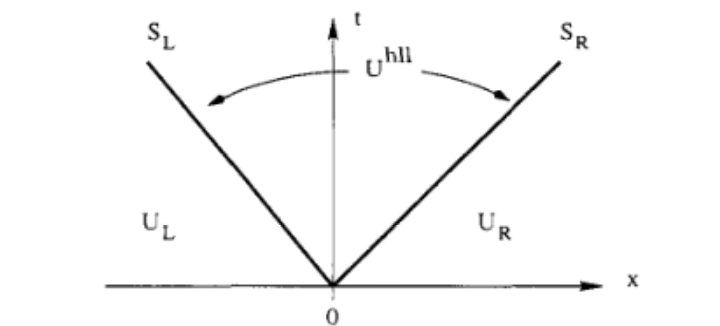
\includegraphics[width=0.5\textwidth]{Figuras/HLL.png}
  \caption{Aproximación de 3 estados distintos en el plano x-t, en el cual se trata de calcular los flujos en la región $U^{hll}$ limitados por las velocidades de señal de la onda}
  \label{fig:HLL}
\end{figure}

\begin{equation}
U \left(x,t \right) = 
\left\lbrace
\begin{array}{rr}
U_L \quad \textup{si} \quad \frac{x}{t}< S_L  \\
U_{hll} \quad \textup{si} \quad S_L< \frac{x}{t} <S_R \\
U_R \quad \textup{si} \quad  \frac{x}{t} > S_R
\end{array}
\right.
\end{equation}

Los flujos $F_R$ y $F_L$ pueden ser calculados directamente ya que solo dependen de $U_R$ y $U_L$ respectivamente pero $F_{hll} \neq F \left( U_{hll} \right)$, asi que resolvemos la integral de la ecuación \ref{ec F_0L} para asi obtener el flujo a traves del eje t

\begin{equation*}
F_{hll} = F_L -S_L U_L+ \frac{1}{T}U_{hll}\left(0- TS_L\right)
\end{equation*}

Entonces
\begin{equation}\label{f_hll 1}
F_{hll} = F_L +S_L \left( U_{hll} -U_L \right)
\end{equation}

Si sustituimos \ref{u_hll} en \ref{f_hll 1} obtenemos:

\begin{equation*}
F_{hll} = F_L +S_L \left( \frac{S_R U_R - S_L U_L + F_L - F_R}{S_R - S_L} -U_L \right)
\end{equation*}
Entonces
\begin{equation*}
F_{hll} = \frac{F_L S_R -F_L S_L+S_L S_R U_R-S_L^2 U_L+S_L  F_L- S_L F_R-S_R S_L U_L + S_L^2 U_L}{S_R-S_L}
\end{equation*}

Eliminando términos semejantes queda
\begin{equation}
F_{hll} = \frac{S_R F_L -S_L F_R + S_L S_R \left(U_R-U_L \right)}{S_R -S_L}
\end{equation}

Con lo que el flujo intermedio de la celda de Gudonov esta dado por:

\begin{equation} \label{fluxesHLL}
F_{i+\frac{1}{2}}^{hll} = 
\left\lbrace
\begin{array}{rr}
F_L \quad \textup{si} \quad 0 \leq S_L  \\
\frac{S_R F_L -S_L F_R + S_L S_R \left(U_R-U_L \right)}{S_R -S_L} \quad \textup{si} \quad S_L \leq 0 \leq S_R \\
F_R \quad \textup{si} \quad  0 \geq  S_R
\end{array}
\right.
\end{equation}

La implementación de esta parte se lleva a cabo en la subrutina \emph{ulax}.

\begin{lstlisting} [frame=single]
  call fluxesHLL(fhll, ghll)
      
        do i=1,nx
          do j=1,ny
            up(:,i,j) = u(:,i,j)                                     &
                        + 0.5*dtx*(fhll(:,i-1,j)-fhll(:,i+1,j))      &
                        + 0.5*dty*(ghll(:,i,j-1)-ghll(:,i,j+1))
          end do
        end do

\end{lstlisting}

Donde \emph{dtx}, \emph{dty} son las derivadas con respecto a \emph{x}, \emph{y} y \emph{fhll}, \emph{ghll} son los flujos calculados con el método de HLL.

La subrutina llama a \emph{fluxesHll}, que es la subrutina que se encarga de calcular los flujos usando el método de HLL, el siguiente código solo es una parte
y solo calcula la ecuación \ref{fluxesHLL}, las variables $i$, $j$ refieren a todos los puntos de la malla, los subíndices \emph{l}, \emph{r}, \emph{u} y \emph{d}
significan izquierda, derecha, arriba y abajo respectivamente y \emph{S} son las velocidades de las ondas mas rápidas de los estados iniciales \emph{U} 
, las variable \emph{dtx} es la derivada con respecto a \emph{x} y \emph{dty} la derivada con respecto a \emph{y}. Para ver toda la subrutina completa ver el apéndice \ref{ap_newrap}

\begin{lstlisting} [frame=single]
  do i=1,nx
  do j=1,ny
    
    if (0 .le. s_l(i,j)) then !less or equal 0<=sl
      fhll(:,i,j)=f_l(:, i,j)

    else if (s_l(i,j) .le. 0 .and. 0 .le. s_r(i,j)) then !sl<=0<=sr
  
      fhll(:,i,j)=(s_r(i,j)*f_l(:,i,j)-s_l(i,j)*f_r(:,i,j)+s_l(i,j)*s_r(i,j)*(u_r(:,i,j)-u_l(:,i,j)))/&
      (s_r(i,j)-s_l(i,j))


    else if (s_r(i,j) .le. 0) then !sr<=0
        fhll(:,i,j)=f_r(:,i,j)

    endif

    if(0 .le. s_d(i,j)) then
      ghll(:,i,j)= g_d(:,i,j)

    else if(s_d(i,j) .le. 0 .and. 0 .le. s_u(i,j)) then

      ghll(:,i,j)=(s_u(i,j)*g_d(:,i,j)-s_d(i,j)*g_u(:,i,j)+s_d(i,j)*s_u(i,j)*(u_u(:,i,j)-u_d(:,i,j)))/&
      (s_u(i,j)-s_d(i,j))

    else if(s_u(i,j) .le. 0) then
        ghll(:,i,j) = g_u(:,i,j)

    endif
  end do
end do
\end{lstlisting}



\section{Ecuaciones de Rankine-Hugoniot}

\subsection{Rankine-Hugoniot Newtoniano}

Ya hemos visto como se resuelven las ecuaciones de la hidrodinámica, pero hay un problema, cuando un jet  choca contra el medio que lo rodea se genera una onda de choque
, esta onda de choque es una discontinuidad de la masa, presión y energía entre el jet y el medio que los rodea. Este problema se ruelve con las ecuaciones de 
Rankine Hugoniot.
Vamos a considerar las relaciones que hay entre los 2 estados que se forman durante una onda de choque. Supongamos que la onda de choque se mueve 
hacia la derecha (ver Figura \ref{fig_move_shock}) sobre un flujo estacionario ($v = 0$) con una velocidad $v_s$, la presión y la densidad, que están enfrente de la onda, son asumidas como
$\rho_0$ y $P_0$ mientras que los flujos que estan comprimidos detras del frente de onda se mueven con una velocidad $v_p$ y que tienen
densidad y presión $\rho_p$, $P_p$.

\begin{figure}
  \centering
  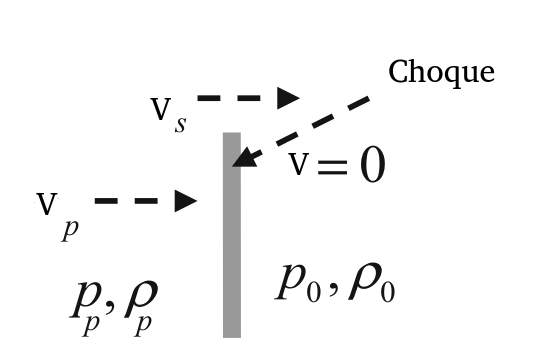
\includegraphics[scale=0.7]{./Figuras/Teoria/move_shock.png}
  \caption{Onda de choque en movimiento sobre un flujo estacionario, tanto la onda como el flujo que esta a la izquierda se mueven a la derecha}\label{fig_move_shock}
\end{figure}
  

Si considerámos nuestro sistema de referencia posicionado sobre la onda (ver Figura \ref{fig_stationary_shock}), usando las transformaciones de Galileo, las direciones de las velocidades
se invierten y la velocidad del flujo que entra al choque es $v_s$ y la que sale es $v_s-v_p$

\begin{figure} 
  \centering
  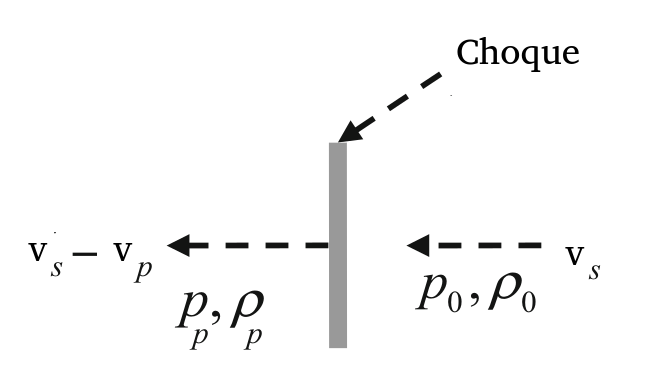
\includegraphics[scale=0.7]{./Figuras/Teoria/stationary_shock.png}
  \caption{Al tomar nuestro sistema de referencia sobre la onda, nuestro choque en movimiento se transforma en una choque estacionario, y los
  flujos que estan a la derecha e izquierda de la onda se mueven hacia la izquierda } \label{fig_stationary_shock}
\end{figure}

Las ecuaciones de Rankine-Hugoniot parten de las ecuaciones de la hidrodinámica considerando un sistema cerrado usando las ecuaciones \ref{conservación_masa_hidrodinamica}, \ref{conservacion_momento_hidrodinamica} y \ref{conservacion_energia_hidrodinamica} donde no varia con el tiempo, es decir, que $\dfrac{\partial}{\partial t}=0$, con lo que se pueden reescribir de la siguiente manera:


La conservación de masa
\begin{equation}
  \nabla \cdot \left( \rho \mathbf{u} \right)=0
\end{equation}

El momento
\begin{equation}
  \nabla \cdot \left( \rho \mathbf{u u} \right) + \nabla p = 0
\end{equation}

Ecuación de la energía

\begin{equation}
 \nabla \cdot \left[ \mathbf{u} \left( e+P \right) \right] = 0
\end{equation}

Considerando una dimensión:

\begin{equation}
\dfrac{d \left( \rho u \right)}{d x} = 0
\end{equation}

\begin{equation}
\dfrac{d \left( \rho u^2 \right)}{d x}+ \dfrac{d P}{d x}=0
\end{equation}

\begin{equation}
\dfrac{d \left( u\left[e +P \right] \right)}{d x} = 0
\end{equation}

Si integramos, la ecuaciones se van a igualar a constantes y podemos reescribir las ecuaciones del siguiente modo usando 
la ecuación de estado $e = \frac{1}{2} \rho u^2 + \frac{P}{\Gamma-1}$ donde $e \left[\frac{\mathrm{erg}}{\mathrm{cm^3}}\right]$ 
es la densidad de energía por unidad de volumen

\begin{equation}\label{RH_masa}
\rho_j u_j = \rho_m u_m
\end{equation}

\begin{equation}\label{RH_momento}
\rho_j u_{j}^{2}+P_j = \rho_m u_{m}^{2}+P_m
\end{equation}

\begin{equation}\label{RH_Energia}
\frac{1}{2} u_{j}^{2}+ \frac{\Gamma}{\Gamma-1} \frac{P_{j}}{\rho_{j}} =
 \frac{1}{2} u_{m}^{2}+ \frac{\Gamma}{\Gamma-1} \frac{P_{m}}{\rho_{m}}
\end{equation}

Donde $\rho \left[\frac{\mathrm{g}}{\mathrm{cm}^3}\right]$ representa la densidad, $u \left[\frac{\mathrm{cm}}{\mathrm{s} }\right]$ la velocidad, 
$P \left[\frac{\mathrm{dyn}}{\mathrm{cm}^2} \right]$ la presión, $\Gamma$ el indice adiabático adimensional donde para velocidades ultrarrelativistas 
$\Gamma = 4/3$ y para no relativistas $\Gamma = 5/3$ y los índices \textit{j, m} que  relacionan a las propiedades del jet y del medio respectivamente. Usando la ecuacion \ref{RH_masa}, podemos definir el flujo como $j \equiv \rho_j u_j = \rho_m u_m$, sustituyendo en la ecuación \ref{RH_momento} podemos reescribirla como:

\begin{equation}\label{RH_momento_j}
P_{j}+\frac{j^2}{\rho_{j}}=P_{m}+\frac{j^2}{\rho_{m}}
\end{equation}

y la ecuación \ref{RH_Energia} llegamos a:

\begin{equation}\label{RH_Energia_j}
\frac{1}{2} \frac{j^{2}}{\rho_{j}^2}+\frac{\Gamma}{\Gamma-1} \frac{P_{j}}{\rho_{j}}=
\frac{1}{2} \frac{j^{2}}{\rho_{m}^2}+\frac{\Gamma}{\Gamma-1} \frac{P_{m}}{\rho_{m}}
\end{equation}

Despejando $j$ de la ecuación \ref{RH_momento_j} obtenemos:
\begin{equation}\label{j^2}
-j^{2}=\frac{P_{j}-P_{m}}{\frac{1}{\rho_{m}}-\frac{1}{\rho_{j}}}
\end{equation}

Ahora sustituyendo la ecuación en \ref{j^2} en \ref{RH_Energia_j} obtenemos:

\begin{equation*}
\frac{1}{2} \left( \frac{P_{m}-P_{j}}{\frac{1}{\rho_{j}}-\frac{1}{\rho_{m}}} \right)
\left(\frac{1}{\rho_{j}^{2}}-\frac{1}{\rho_{m}^{2}} \right)
=
\frac{\Gamma}{\Gamma-1}
\left( \frac{P_{m}}{\rho_{m}}-\frac{P_{j}}{\rho_{j}} \right)
\end{equation*}

$\Rightarrow$

\begin{equation*}
\frac{1}{2}	\left( P_{m} - P_{j} \right)
\left( \frac{1}{\rho_{j}}+\frac{1}{\rho_{m}} \right)
=
\frac{\Gamma}{\Gamma-1}
\left( \frac{P_{m}}{\rho_{m}}-\frac{P_{j}}{\rho_{j}} \right)
\end{equation*}

$\Rightarrow$

\begin{equation*}
\frac{1}{\rho_{m}} \left( \frac{1}{2} P_{m}- \frac{1}{2} P_{j}-
\frac{\Gamma}{\Gamma-1} P_{m} \right)
=
\frac{1}{\rho_{j}} \left( \frac{1}{2} P_{j}- \frac{1}{2} P_{m}-
\frac{\Gamma}{\Gamma-1} P_{j} \right)
\end{equation*}

$\Rightarrow$

\begin{equation*}
\frac{1}{\rho_{m}} \left[  \left(\frac{\Gamma + 1}{\Gamma - 1} \right) P_{m} + P_{j} \right]
=
\frac{1}{\rho_{j}} \left[  \left(\frac{\Gamma + 1}{\Gamma - 1} \right) P_{j} + P_{m} \right]
\end{equation*}

Con lo que nos queda:

\begin{equation}\label{RH_no_rel_choque_no_fuerte}
\frac{\rho_{m}}{\rho_j} =
\frac{\left( \Gamma +1 \right) P_{m}+ \left( \Gamma -1 \right) P_{j
}}{\left(\Gamma +1 \right) P_{j}+ \left( \Gamma -1 \right) P_{m}}
= \frac{u_j}{u_m}
\end{equation}

Si consideramos choque fuerte, es decir, $P_j \gg P_m$, implicaría que $P_m \simeq 0$, por lo que

\begin{equation}
\rho_j = \frac{\Gamma +1}{\Gamma-1} \rho_m 
\end{equation}
Tomando a $\Gamma = 5/3$ da

\begin{equation}
\rho_j = 4 \rho_m
\end{equation}

\begin{equation}
u_j = \frac{1}{4} u_m
\end{equation}

\begin{equation}
P_{j} = \frac{3}{4}\rho_m u_m^{2}
\end{equation}




\subsection{Rankine-Hugoniot Relativista}

% Si suponenmos las condiciones de Rankine-Hugoniot en un jet relativista, la presión interna del jet va a a ser mucho más grande que la del medio que lo está
% rodeando. Si colocamos nuestro marco de referencia sobre el jet, su masa será:

% \begin{equation}
%   M = \pi \rho v_j R^2 t
% \end{equation}

% Donde $M$, $\rho$, $v_j$ y $R$ son la masa, densidad, velocidad y radio del jet respectivamente, $t$ es el tiempo. Si multiplicamos todo por $c^2$,
% que es la velocidad de la luz al cuadrado, obtenemos la energía.

% \begin{equation}
%   E = Mc^2 = \pi \rho v_j R^2 t c^2
% \end{equation}



% Como tenemos nuestro sistema de referencia en la onda de choque inicial ($\gamma_j$) sobre nuestro objeto compacto. La energía del jet es:
% \begin{equation}
%   E = \gamma_{\infty} E
% \end{equation}
% Donde $\gamma_{\infty}$ es factor de lorentz con el que se mueve el jet cuando ya se ha alejado del objecto compacto.
% Y si ahora nos movemos al sistema de referencia visto desde la Tierra, la energía se vuelve:



% \begin{equation}
%   E = \gamma_{j} \gamma_{\infty} E_j
% \end{equation}

% Donde $\gamma_j$ es el factor de lorentz del jet y $E_j$ es la energía 
% del jet.

% Si derivamos con respecto al tiempo obtenemos la luminosidad.


% \begin{equation}
%   L = \dfrac{dE}{dt} = \gamma_{j} \gamma_{\infty}  \pi \rho v_j R^2 c^2
% \end{equation}

% Podemos obtener la densidad del jet despejando $\rho$ de la anterior ecuación

% \begin{equation}
%   \rho_j = \frac{L}{\gamma_{j} \gamma_{\infty}  \pi v_j R^2 c^2}
% \end{equation}

Considerando la conservación de masa:

\begin{equation}
  \rho_j v_j \gamma_j=  \rho_{\infty} v_{\infty} \gamma_{\infty}
\end{equation}

Donde $v_j$, $v_\infty$ es la velocidad del jet y del medio que lo rodea respectivamente, despejando $\rho_{\infty}$ obtenemos:

\begin{equation}\label{eq_masa_densidad_despejada}
  \rho_\infty = \rho_j \frac{v_j \gamma_j }{v_\infty \gamma_\infty}
\end{equation}

Si ahora consideramos la ecuación de momentos

\begin{equation}
  \left( e_j + P_j\right) v^2_j \gamma^2_j + P_j = \left( e_{\infty} + P_{\infty}\right) v^2_{\infty} \gamma^2_{\infty} + P_{\infty}
\end{equation}

La densidad de energía se compone de la energía interna del sistema y de la energía cinética

\begin{equation} \label{eq_densidad_de_energia}
  e = e_{int} + e_k
\end{equation}

La energía interna para un sistema ultra-relativista es $ P = \frac{1}{3}e_{int}$ lo que implica que $e_{int} = 3P$, mientras que la densidad de energía
cinética es $e_k = \rho c^2$ pero como estamos considerando a $c = 1$ esto se reduce a $e_k = \rho$. Si sustituimos todo esto en la ecuación
\ref{eq_densidad_de_energia} entonces nos queda:

\begin{equation} \label{eq_momentos_relativista_modificada}
  \left( \rho_j + 4P_j \right) v^2_j \gamma^2_j  +P_j = \left( \rho_\infty + 4P_\infty \right) v^2_{\infty} \gamma^2_{\infty}  +P_\infty
\end{equation}

Con la ecuación \ref{eq_masa_densidad_despejada} podemos modificar la ecuación \ref{eq_momentos_relativista_modificada}, con lo que nos queda:

\begin{equation}
  \left( \rho_j + 4P_j \right)v_j \gamma^2 +P_j = \left( \rho_\infty + 4P_\infty \right)v_\infty \gamma^2 +P_\infty
\end{equation}

y tomando un choque fuerte $P_j \gg P_\infty $ Podemos reducir la ecuación a 

\begin{equation} \label{eq_momentos_choque_fuerte}
  \left( \rho_j + 4P_j \right)v_j^2 \gamma^2 +P_j =  \rho_\infty  v_\infty^2 \gamma_{\infty}^{2} 
\end{equation}

Sustituyendo la ecuación \ref{eq_masa_densidad_despejada} en \ref{eq_momentos_choque_fuerte} obtenemos

\begin{equation} \label{eq_momentos_choque_fuerte}
  \left( \rho_j + 4P_j \right)v_j^2 \gamma^2 +P_j = \rho_j v_j v_\infty \gamma_j \gamma_\infty
\end{equation}

Suponiendo $\left( \rho_j + 4P_j \right)v_j^2 \gamma^2 \gg P_j $



\begin{equation}
  \left( \rho_j + 4P_j \right)v_j \gamma_j = \rho_\infty v_\infty  \gamma_\infty
\end{equation}

Despejando la presión obtenemos

\begin{equation}
  P_j = \frac{\rho_j}{4}\left(\frac{v_\infty}{v_j} \frac{\gamma_\infty}{\gamma_j}-1\right)
\end{equation}

Como $v_j \thickapprox v_\infty \thickapprox c$

\begin{equation}
  P_j = \frac{\rho_j}{4}\left( \frac{\gamma_\infty}{\gamma_j}-1\right)
\end{equation}

Para poder simular las condiciones de un jet, necesitamos saber la densidad, velocidad y presión del mismo, como los jet tienen velocidades cercanas a la
de la luz, se pueden tomar valores cercanos a esta constante. La densidad se obtendá en la siguiente sección 


\subsection{Luminosidad}
Si suponenmos las condiciones de Rankine-Hugoniot en un jet relativista y si colocamos nuestro marco de referencia sobre el jet, la energía será:

\begin{equation} \label{eq._energia_relativista}
  E = \gamma_{\infty} M c^2
\end{equation}

Donde $\gamma_{\infty}$ es factor de lorentz con el que se mueve el jet cuando ya se ha alejado del objecto compactoy como sabemos 
que $L \equiv \dfrac{d E}{d t}$ entonces derivando la ecuación \ref{eq._energia_relativista} respecto al tiempo

Entonces tenemos 

\begin{equation} \label{eq._luminosidad_relativista}
  \dfrac{d E}{d t} = \gamma_{j} \dot{ M }  c^2
\end{equation}

La taza de flujo de masa $\dot{M}$ se puede escribir como

\begin{equation}
  \dot{M} = \rho_j u_j A_j
\end{equation}

Donde $\rho$ es la densidad, $u_j = v_j \gamma_{j}$ es la cuadrivelocidad,  y $A_j$ es el área, que en este caso, corresponde la parte esférica del jet
entonces la luminosidad se puede escribir como:

\begin{equation}
  L \equiv \dfrac{d E}{d t} = 4\pi r_j^2 \rho_j v_j \gamma_j \gamma_{\infty} c^2
\end{equation}

Despejando la densidad

\begin{equation}
  \rho = \frac{L}{4\pi r_j^2 v_j \gamma_j \gamma_{\infty} c^2}
\end{equation}

Al obtener la densidad ya podemos simular el jet dado que la luminosidad se puede obtener de detectores de Rayos $\gamma$ y las velocidades tambien ? preguntar a 
Diego


\section{Ecuaciones de Sedov-Taylor por soluciones} \label{seccion_ecuaciones_de_sedov_taylor}

Una forma de verificar si nuesto código funciona es usar el problema de Sedov-Taylor, que básicamente es modelar una onda de choque esférico con una determinada 
energía, presión y densidad sobre un medio externo. 
Una onda de choque se produce cuando se libera una gran cantidad de energía E, en un fluido con densidad $\rho_w$, la cual crea explosiones muy violentas. 
Este tipo tipo ocurre muy a menudo en el universo. Este tipo de problemas son conocidos como explosiones de Sedov-Taylor. Este problema puede servir para testear mi código debido a que podemos resolver analíticamente el problema y compararlo con el método númerico.

\subsection{Aproximación en funcion del analisis dimensional}
Si consideramos un choque fuerte,
es decir, $P_w \gg P_m$,
entonces las únicas variables que podemos tomar son $E$, $\rho_w$ y $t$ que es el tiempo.
Las dimensiones de estas cantidades son 

\begin{equation}
  \left[ \rho_w \right] = \frac{M}{L^3}
\end{equation}

\begin{equation}
  \left[E\right] = M \frac{L^2}{T^2}
\end{equation}

\begin{equation}
  \left[ t\right] = T
\end{equation}

La única cantidad que se puede construir que contenga la energía el tiempo y la densidad y que su dimensión sea
la longitud es:

\begin{equation}
  \left[ \left( \frac{Et^2}{ \rho_w } \right)^{\frac{1}{5}}\right] = L
\end{equation}

Por lo que para cualquier radio de onda de cualquier choque, debe depender de estas variables

\begin{equation}
  R(t) = \eta  \left( \frac{Et^2}{ \rho_w } \right)^{\frac{1}{5}} \varpropto t^{\frac{2}{5}}
\end{equation}

Por lo que la constante $\eta$ debe ser de la siguiente manera

\begin{equation}
  \eta \equiv \frac{r}{\left( \frac{Et^2}{\rho_w} \right)^{\frac{1}{5}}}
\end{equation}



\subsection{Aproximación en funcion de la conservación de la energia}

Otra aproximación es buscando el cociente de presiones y densidades en función del número Mach.
Podemos estimar el radio $R(t)$ de una onda de choque en función del tiempo, sabemos que el volumen de una esfera es $V = \frac{4}{3} \pi * R^3$ y
la densidad de la onda es constante entonces el volumen $V = \frac{M}{\rho_w}$. La velocidad media de la onda es $v(t) \sim \frac{R(t)}{t} $
entonces podemos aproximar la energía cinética de la onda como 

\begin{equation}
	E_{kin} \sim \frac{1}{2} M v^2 \sim \rho_w R^3 \left( \frac{R}{t} \right) ^2 = \rho_w \frac{R^5}{t^2}
\end{equation}

Ahora la energía térmica de una explosion es 

\begin{equation} \label{eq_energia_termica}
	E_{th} \sim \frac{3}{2}PV
\end{equation}

Para encontrar la presión, primero defineremos algunas ecuaciones antes.

La entalpia estancada se define en términos de la entalpia y la velocidad de la onda 

\begin{equation}
	h_0 = h + \frac{1}{2} v^2
\end{equation}

La cual la podemos rescribir como

\begin{equation} \label{eq_entalpia}
	h_0 = h + \left( 1 +\frac{1}{2} \frac{v^2}{h} \right)
\end{equation}

Ahora sabemos que la velocidad del sonido puede ser definida como 

\begin{equation} \label{eq_sonido_1}
	a = \sqrt{\frac{\Gamma P}{\rho}}
\end{equation}

y tambien como 

\begin{equation} \label{eq_sonido_2}
	a = \sqrt{(\Gamma-1) h}
\end{equation}

Donde $a$ es la velocidad del sonido, $h$ la entalpia, $v$ la velocidad, $P$ la presión y $\rho$ la densidad. Tambien definimos el número de Mach como 

\begin{equation} \label{eq_Mach}
	M = \frac{v}{a}
\end{equation}

Si combinamos la ecuación \ref{eq_sonido_1} con la ecuación \ref{eq_Mach} y lo sustituimos en la ecuación \ref{eq_entalpia} nos queda la entalpia en funcion de la velocidad de la onda y del sonido

\begin{equation} \label{h_0_funcion_aire_mach}
	h_0 = \frac{a^2}{\Gamma - 1} \left( 1 + \frac{\Gamma - 1}{2} M^2 \right)
\end{equation}

Esta ecuacion servirá más adelate. Volviendo a las ecuaciones de Rankine Hugoniot podemos usar la ecuacion
\ref{RH_Energia} y \ref{entalpia_funcion_presion_densidad} para obtener la ecuacion de la energía en funcion de la entalpia, lo que nos va a quedar al final como

\begin{equation}\label{RH_entalpia}
  h_w +\frac{1}{2}v_w^2 = h_w +\frac{1}{2}v_w^2
\end{equation} 


Donde $ h $ es la entalpia y $v$ la velocidad, los sub-índices $w$, $m$ corresponden a la onda y al medio respectivamente.

Si dividimos la ecuación \ref{RH_momento} entre \ref{RH_masa}, y cambiando los sub-índices $j$ por $w$
obtenemos la siguiente ecuación 

\begin{equation} \label{RH_momento_masa}
  v_w + \frac{P_w}{\rho_w v_w} = v_m + \frac{P_m}{\rho_m v_m}
\end{equation}

Usando la ecuación \ref{eq_sonido_1} en la ecuación \ref{RH_momento_masa} podemos reescribir la ecuación de 
la siguiente manera:

\begin{equation} \label{eq_diferencia_velocidades}
  v_w-v_m = \frac{1}{\Gamma} \left(\frac{a_m^2}{v_m} - \frac{a_w^2}{v_w} \right)
\end{equation}

Por simplicidad definimos la entalpia estancada como 

\begin{equation}
  h_w + \frac{1}{2} v_w = h_w + \frac{1}{2} v_w \equiv h_0
\end{equation}

Por lo que podemos definir a la velocidad del sonido como:

\begin{equation} \label{eq_sonido_onda}
  a_w = \left( \Gamma-1 \right) h_w = \left( \Gamma-1 \right) \left( h_0 -\frac{1}{2} v_w^2 \right)
\end{equation}

\begin{equation} \label{eq_sonido_medio}
  a_m = \left( \Gamma-1 \right) h_m = \left( \Gamma-1 \right) \left( h_0 -\frac{1}{2} v_m^2 \right)
\end{equation}

Sustituyendo las ecuaciones \ref{eq_sonido_onda} y \ref{eq_sonido_medio} en la ecuación \ref{eq_diferencia_velocidades}
nos queda

\begin{equation}
  v_w-v_m = \frac{\Gamma - 1}{\Gamma} \left[ \frac{h_0}{v_m} - \frac{h_0}{u_w} + \frac{1}{2} \left( v_w - v_m\right) \right]
\end{equation}

Dividiendo por $ \left( v_w - v_m \right)$

\begin{equation}
  1 = \frac{\Gamma - 1}{\Gamma} \left( \frac{h_0}{v_m v_w} + \frac{1}{2} \right)
\end{equation}

Que al final la podemos reescribir como

\begin{equation} \label{eq_denominador}
  \frac{1}{v_w v_m} = \frac{1}{\left( \Gamma -1\right) h_0} \frac{\Gamma + 1}{2}
\end{equation}

Otra ecuación que nos va a servir es la definicion de Mach ya que como

\begin{equation}\label{velocidad_aire_mach}
  v_w^2 = a_w^2 M_w^2
\end{equation}

Entonces usando \ref{h_0_funcion_aire_mach} podemos reescribir la ecuación \ref{velocidad_aire_mach} como
como

\begin{equation} \label{eq_numerador}
  v_w^2 = M_w^2 \frac{\left( \Gamma -1 \right) h_0}{1+\frac{\Gamma - 1}{2} M_w^2}
\end{equation}

Usando la ecuación de momentos \ref{RH_masa} podemos reescribirla como

\begin{equation} \label{eq_fraccion_momentos}
  \frac{\rho_m }{\rho_w} = \frac{ v_w}{v_m} = \frac{v_w^2}{v_w v_m}
\end{equation}

Como ya sabemos cuanto vale el numerador (ec. \ref{eq_numerador}) y el denominador (ec. \ref{eq_denominador})
de la fracción, podemos definir el cociente de las densidades \ref{eq_fraccion_momentos} como 

\begin{equation}\label{eq_fraccion_momentos_funcion_mach}
  \frac{\rho_m}{\rho_w} = \frac{\left( \Gamma +1 \right) M_w^2}{2+ \left( \Gamma -1 \right) M_w^2}
\end{equation}

Entonces para encontrar las presiones combinamos las ecuaciones \ref{RH_momento} y \ref{RH_masa} tenemos

\begin{equation}
  P_m - P_w = \rho_w v_w^2 - \rho_m v_m^2 = \rho_w v_w^2 \left( 1 - \frac{v_m}{v_w}\right) = \rho_w v_w^2 \left( 1 - \frac{\rho_w}{\rho_m}\right)
\end{equation}

Usando la siguiente relación $\rho v^2 = \Gamma P M^2$, que se obtiene de las ecuaciones \ref{eq_sonido_1} y
\ref{eq_Mach},dividiendo por $P_w$ y sustituyendo  $\frac{\rho_m}{\rho_w}$ de la ecuación \ref{eq_fraccion_momentos_funcion_mach}
nos queda

\begin{equation} \label{eq_fraccion_Presiones}
  \frac{P_m}{P_w} = 1 + \frac{2 \Gamma}{\Gamma + 1} \left( M_w^2 -1\right)
\end{equation}

Usando la siguiente relación $ P_w = \frac{\rho a_w }{\Gamma}$ se puede obtener el límite del choque fuerte

\begin{equation}
  P_m  \simeq \frac{2 \rho_w v_w^2}{\Gamma + 1}
\end{equation}

Con esto ya podemos obtener la energía térmica de la ecuación \ref{eq_energia_termica} por lo que nos queda 

\begin{equation}
  E_{th} \sim P_m R^3 \sim \rho_w v_w^2 R^3 \sim \rho_w \frac{R^5}{t^2}
\end{equation}

Como tiene el mismo orden que el de la energía cinética, entonces la energía total que es una cantidad conservada, se espera que

\begin{equation}
  E_t = E_{kin} + E_{th} \sim \rho_w \frac{R^5}{t^2}
\end{equation}

Despejando el radio, obtenemos lo siguiente

\begin{equation} \label{eq_Radio_proporcional}
  R(t) \varpropto \left(\frac{E t^2}{\rho_w}\right)^{\frac{1}{5}}
\end{equation}

Vemos que la Figura \ref{fig_Radio_v_tiempo} parece una funcion logaritmica y su radio de expansion no crece muy rápidamente conforme avanza el tiempo,
Para tiempos $t = 4$ y $t = 100$, el radio es $R = 1.74$ y $R = 6.30$ respectivamente

\begin{figure}
  \centering
    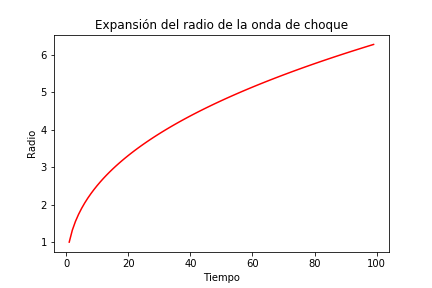
\includegraphics[width=0.5\textwidth]{Figuras/Teoria/Radio_vs_tiempo.png}
  \caption{Radio de expansión de una onda de choque conforme avanza el tiempo } \label{fig_Radio_v_tiempo}
\end{figure}

Si derivamos la ecuación \ref{eq_Radio_proporcional}, obtenemos la velocidad

\begin{equation}
  \dfrac{de}{dt} = \frac{2}{5}\frac{R(t)}{t} \varpropto t^{\frac{-3}{5}}
\end{equation}


A diferencia del radio, la velocidad, se asemeja más a una asíntota que decrece muy rápidamente (ver \ref{fig_velocidad_vs_radio})

\begin{figure}
  \centering
    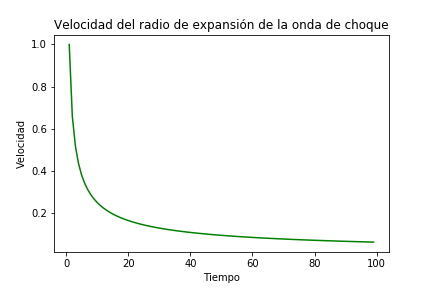
\includegraphics[width=0.5\textwidth]{Figuras/Teoria/Velocidad_vs_tiempo.png}
  \caption{Velocidad del radio de expansión de una onda de choque conforme avanza el tiempo } \label{fig_velocidad_vs_radio}
\end{figure}



% ======================================NUEVO CAPITULO ================================================
% ======================================NUEVO CAPITULO ================================================
% ======================================NUEVO CAPITULO ================================================
% ======================================NUEVO CAPITULO ================================================

\chapter{Verificación del código}


\section{Pruebas unidimensionales}

Para tener la seguridad de que el código hidrodinámico funcione bien se realizaron pruebas 
unidimensionales (1D)
de un tubo de Sod ya sea en el régimen newtoniano así como en el relativista (en ambos régimenes se usó
el método de Lax así como el HLL, y se compararon los resultados con la solución analítica). 
Estas pruebas consisten en determinar como se comporta un gas ideal en un tubo 1D 
el cual se tiene inicialmente una discontinuidad. Antes de un valor determinado crítico el gas tiene ciertos 
valores para la densidad, velocidad y presión, y a partir ese punto crítico el gas tiene distintos 
valores.

% Para validar que el código realmente funciona se implementará un explosión esférica como la que se trata en las ecuaciones de Sedov-Taylor. Como
% este problema es hidrodinámico, tenemos que ver que el radio de la onda de choque se expanda como $t^{0.4}$. Las simulaciones se programaróna para 
% que corriera de un tiempo $t = 0$ s hasta $t = 9.6 \times 10^{10}$ s
% Los valores del choque esférico estan dados en la tabla \ref{Tabla_parametros_sedov}
% $\rho = 3.48 x 10^{-24} $ $\mathrm{g} \, \mathrm{cm}^{-3}$, la presión $P = 2.01 x 10^{-6} $ $\mathrm{dyn}$, se tomo un radio de 2 pc.
% Los valores para el medio que rodean la onda de choque fue $\rho = 1.67 \, x \, 10^{-24} $ $\mathrm{g} \, \mathrm{cm}^{-3}$ y 
% la presión $P = 8.97 x 10^{-10} $ $\mathrm{dyn}$


\subsection{Casos newtonianos}

Para las pruebas newtonianas se usaron los valores del cuadro 
\ref{Cuadro_parametros_sod_tube}. El primer  caso (denominado caso 1 newtoniano), produce una onda 
de rarefacción que se mueve a la izquierda y una onda de choque\footnote{
  Una onda de rarefacción es la progresión de partículas que se aceleran lejos de una zona 
  comprimida. Siempre se mueven a regiones de mayor densidad y no presentan discontinuidades, mientras que
  una onda de choque se moverá siempre a las zonas de menor densidad y presentará discontinuidades además
  de que su valor siempre será una constante. Dado que para el primer caso tendremos valores de densidad
  y presión más grandes que el lado derecho de la posición crítica ($x_0$), 
  podemos decir que del lado izquierdo 
  de $x_0$ será una una onda de rarefacción que se moverá a la izquierda, mientras que del lado
  derecho será una onda de choque que se moverá a la derecha.
  
} que se mueve a la derecha. La condición inicial gas consiste en tener el dominio 
unidimensional dividido a la mitad del dominio (en $x_0$) con ciertos valores de densidad ($\rho_l$), 
velocidad ($v_l$) y presión ($p_l$) del lado izquierdo\footnote{Los subíndices \emph{l} y \emph{r} 
vienen del ingĺés \emph{left} y \emph{right} que significan izquierda y derecha respectivamente.}, 
mientras que del lado derecho tendrán densidad ($\rho_r$), velocidad ($v_r$) y  presión ($p_r$). 
La elección del índice adiabático $\Gamma = 7/5$ se dio para poder simular y comparar los mismos modelos que 
mostrados por  Lora-Clavijo \emph{et al.} (2013).

\begin{table}[htbp]
  \begin{center}
  \begin{tabular}{|c|c|c|c|c|c|c|}
  \hline 
  \textbf{Caso} & \textbf{$p_l$} [$\text{dyn}/\text{cm}^2$] & \textbf{$p_r$} [$\text{dyn}/\text{cm}^2$]& \textbf{$v_l$} [$\text{cm}/\text{s}$]& \textbf{$v_r$} [$\text{cm}/\text{s}$]& \textbf{$\rho_l$} [$\text{g}/\text{cm}^3$]& \textbf{$\rho_r$} [$\text{g}/\text{cm}^3$] \\ 
  \hline 
  Caso 1 & 1.0  & 0.1  & 0.0 & 0.0 & 1.0  & 0.125 \\ 
  \hline 
  Caso 2 & 0.4  & 0.4  & -1.0 & 1.0 & 1.0  & 1.0  \\ 
  \hline 
  \end{tabular}
  \caption{\label{Cuadro_parametros_sod_tube} Valores iniciales de la presión ($p$), velocidad ($v$)
  y densidad ($\rho$), del lado izquierdo ($p_l, v_l, \rho_l$) y derecho ($p_r, v_r, \rho_r$)
  para los casos newtonianos. Para todos los
  casos el dominio espacial será $x \in [0,1]$ cm, la posición crítica sería
  $x_0 = 0.5$ cm y un índice adiabático $\Gamma = 7/5$}
  \end{center}
\end{table}


En la Figura \ref{caso_new_rar_shock} se muestra la evolución temporal de la densidad, 
presión y velocidad para el caso 1 newtoniano usando el método Lax. En la Figura se ve como 
una onda de choque viaja hacia la derecha a través de la región de alta densidad.
En el panel superior izquierdo
notamos como para 0.2 segundos el perfil de densidad $\rho$ tiene dos brincos situados 
aproximadamente en 
x=0.70 cm, donde la densidad ($\rho \approx 0.48 \,  \text{g}/ \text{cm}^3$), 
cambia su densidad a $\rho \approx 0.28 \,  \text{g}/ \text{cm}^3$, la velocidad y la presión 
mantienen los mismos valores 
($v \approx 0.99$ cm/s y $p \approx 0.3 \,  \text{dyn}/ \text{cm}^2 $).
En x=0.85 cm, la velocidad ($v \approx 0.99$ cm/s), la presión 
($p \approx 0.3  \,  \text{dyn}/ \text{cm}^2 $)  y La densidad 
($\rho \approx 0.28 \,  \text{g}/ \text{cm}^3$) 
tienen una discontinuidad y cambian sus valores a los iniciales del estado derecho del tubo
que no han sido afectados por la onda. 
La primera discontinuidad hace referencia a la onda de contacto que tiene la misma velocidad
que que los estados de la izquierda y la derecha $V_c = v_l = v_r$ donde $V_c$
es la velocidad de la onda de contacto por lo que esto hace que las presiones sean iguales 
$p_l = p_r$. Esta primera discontinuidad solo se 
presenta en el panel de las densidad, la otra discontinuidad que se presenta en los 3 páneles es la 
discontinuidad de la onda de choque.

Para el tiempo t=0.4 s
discontinuidad de la onda de choque ya no se presenta en nuestro dominio de los 3 páneles, mientras 
que la cabeza de la onda de rarefacción todavia se muestra en $x \approx 0.01$ cm. La única discontinuidad 
presente es la de onda de 
contacto, donde $\rho \approx 0.48 \,  \text{g}/ \text{cm}^3$ únicamente cambia su valor 
a $\rho \approx 0.28 \,  \text{g}/ \text{cm}^3$, y la velocidad $v \approx 0.99$ cm/s y 
presión $p \approx 0.3 \,  \text{dyn}/ \text{cm}^2 $ mantienen
sus mismos valores.
% Esta onda es más lenta que la de rarefacción ya que se encuentra en $x \approx 0.85$ cm.

  \begin{figure}
    \centering
        \subfigure{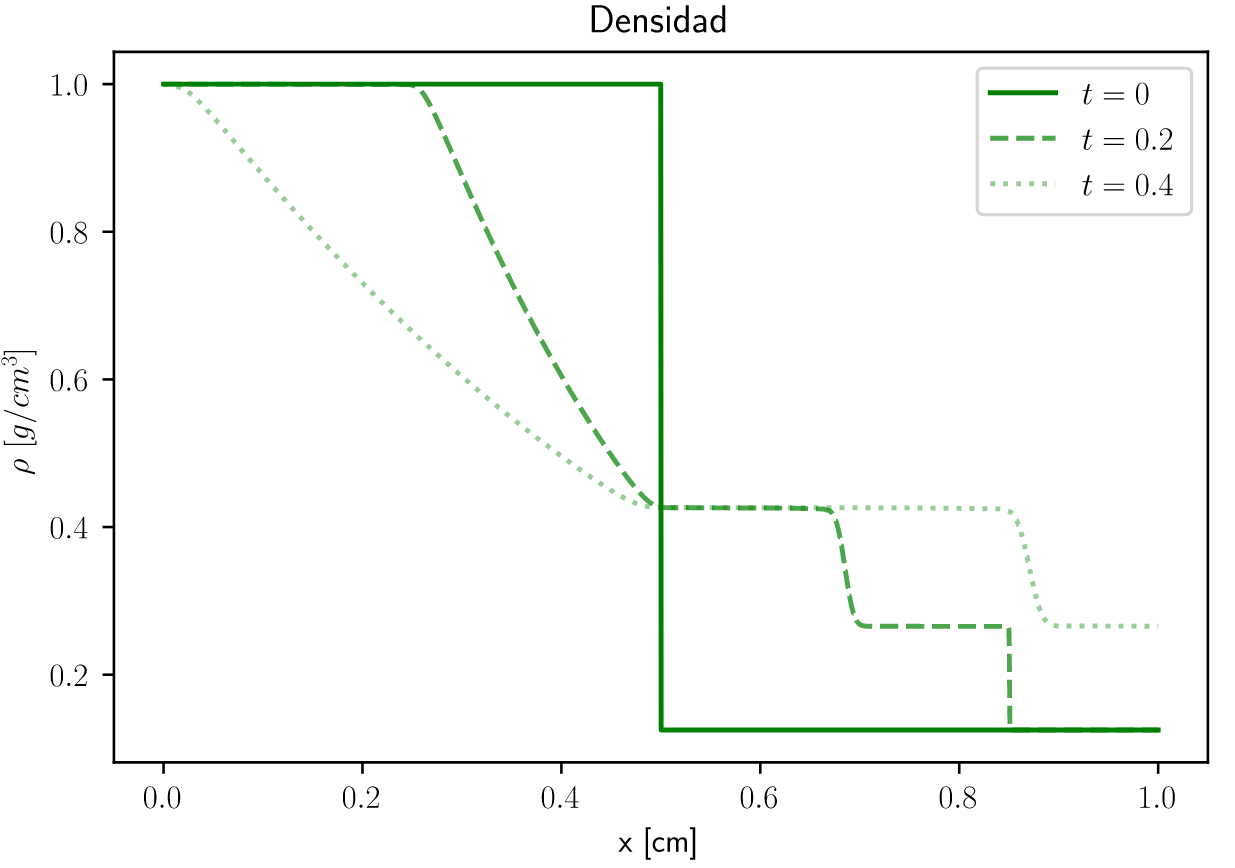
\includegraphics[scale = 0.16]{./Figuras/verificacion_del_codigo/caso_newtoniano/caso_new_rar_shock_rho.png}}
        \subfigure{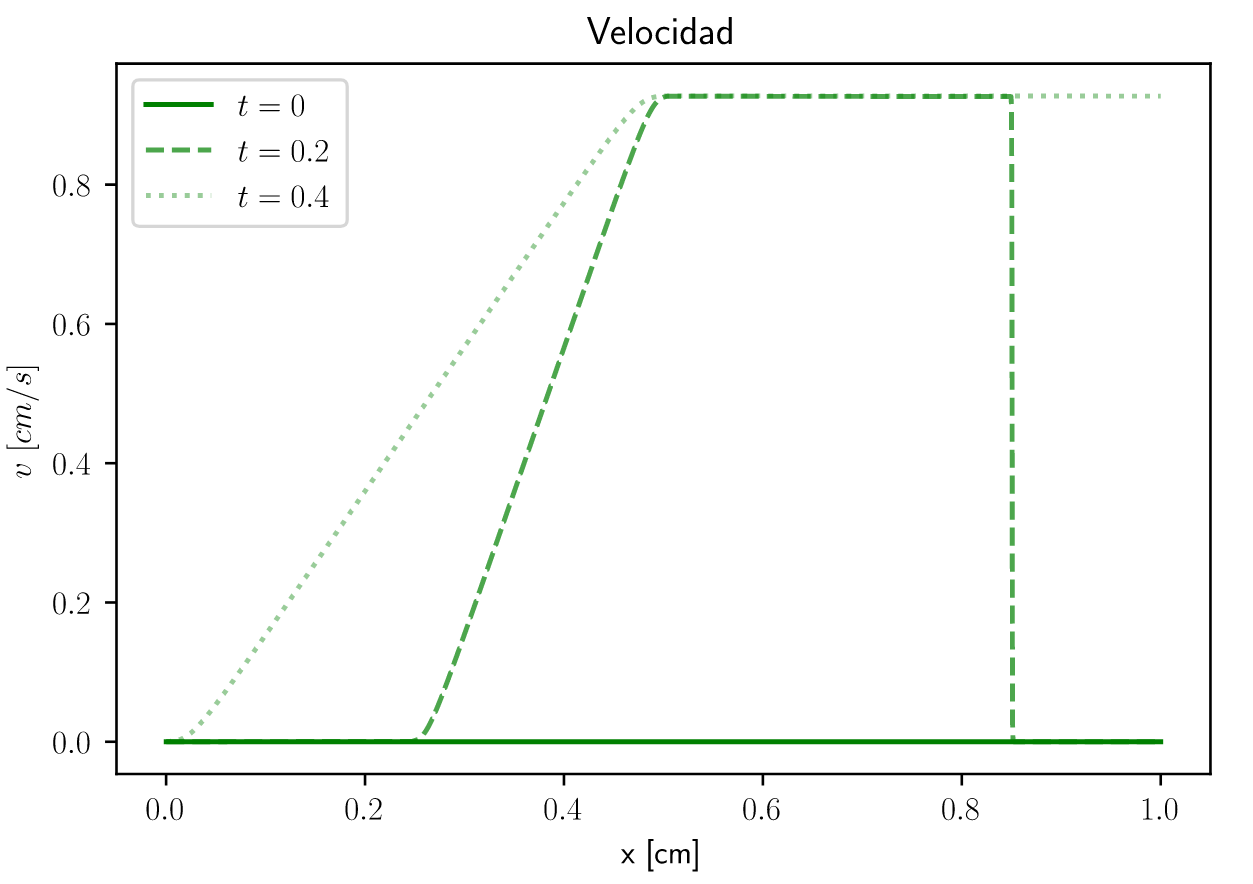
\includegraphics[scale = 0.16]{./Figuras/verificacion_del_codigo/caso_newtoniano/caso_new_rar_shock_v.png}}
        \subfigure{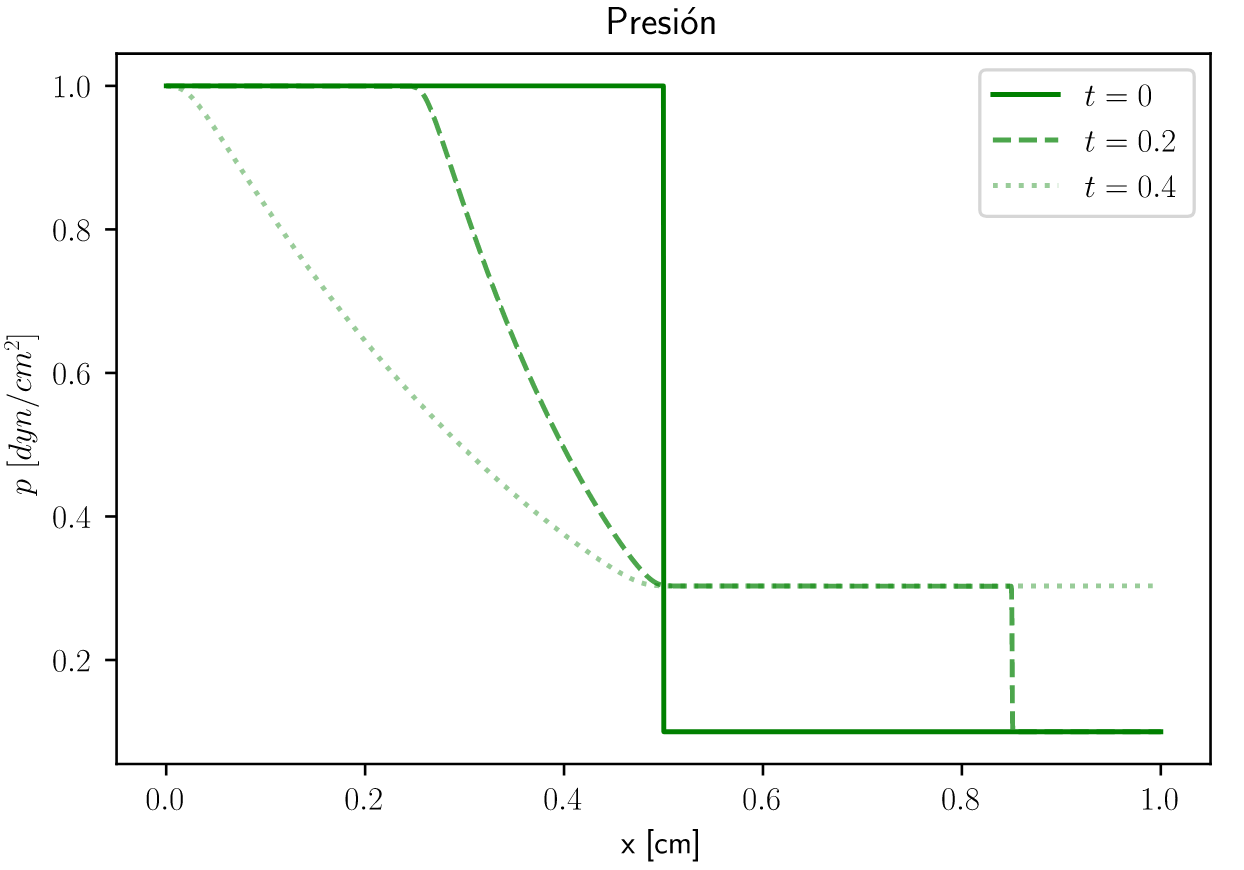
\includegraphics[scale = 0.16]{./Figuras/verificacion_del_codigo/caso_newtoniano/caso_new_rar_shock_p.png}}
      \caption{\label{caso_new_rar_shock} Evolución temporal del caso 1 newtoniano (usando el método Lax) donde se muestra
      las magnitudes de densidad (arriba a la izquierda), presión (abajo) y 
      velocidad (arriba a la derecha). 
      Se usó un índice adiabático $\Gamma = 7/5$ .}
  \end{figure}

  El caso 1 newtoniano tambien fue resuelto utilizando el método HLL y usando varias resoluciones. 
  En la Figura 
  \ref{comparacion_analitico_newtoniano_caso_1}, se muestra la comparación entre los métodos Lax 
  y HLL a 10,000 píxeles. 
  El panel de arriba a la izquierda muestra la densidad $\rho = 1.0 \,  \text{g}/ \text{cm}^3$ 
  donde presenta un cambio en 
  $x \approx 0.24 $ cm y baja gradualmente hasta $x \approx 0.48$ cm donde la densidad ahora es $\rho \approx
  0.45 \,  \text{g}/ \text{cm}^3$. Podemos ver que tanto Lax y HLL tiene los mismos valores que el método analítico. 
  Para las discontinuidades en $x \approx 0.74$ cm (contacto) y $x \approx 0.93$ cm (choque) cambian los valores de densidad $
  \rho \approx 0.48 \,  \text{g}/ \text{cm}^3$ a $\rho \approx 0.35 \,  \text{g}/ \text{cm}^3$ y 
  después a $\rho =0.1 \,  \text{g}/ \text{cm}^3$ 
  respectivamente. Aquí podemos ver
  tanto Lax como HLL presentan dificultad con la discontinuidad de contacto, 
  pero logra adaptarse muy bien para la discontinuidad de choque, en si ambos métodos reproducen a 
  la perfección toda la región donde se desarrolla la discontinuidad en resoluciones de 10,000 píxeles
  sobre todo en los valores que son constantes y los que cambia ya sea lineal o parabólicamente.
  En el panel de arriba a la derecha se muestra la velocidad, esta, al igual que la densidad cambian 
  sus valores gradualmente de $v = 0$ cm/s en $x \approx 0.20$ cm a $v \approx 0.99$ cm/s en 
  $x \approx 0.50$ cm,
  donde se mantiene contante hasta la discontinuidad de choque en $x \approx 0.93$ cm y regresa a $v = 0$ cm/s.
  En este punto, tanto Lax como HLL, no tiene ninguna dificultad al reproducir a discontinuidad de 
  choque.
  El panel de abajo a la izquierda es la presión, el cual cambia su valor 
  $p = 1.0 \,  \text{dyn}/ \text{cm}^2 $ en $x \approx 0.48$ cm
  bajando hasta $p = 0.4 \,  \text{dyn}/ \text{cm}^2 $ en $x \approx 0.48$ cm, 
  donde igual que la velocidad
  mantiene su mismo valor hasta $x \approx 0.93$ cm donde su valor decae a $p = 0.1 \,  \text{dyn}/ \text{cm}^2 $



{\color{red}El panel de abajo a la derecha de la Figura 
\ref{comparacion_analitico_newtoniano_caso_1} muestra la solución analítica así como los resultados 
obtenidos usando Lax con distintas resoluciones ($nx = 10^2, \, 10^3, \,10^4$).Queda claro como 
conforme se incrementa la resolución (píxeles\footnote{Para fines prácticos, usaremos la palabra "píxel" para describir los $\Delta x$ en 
las que se divide nuestro dominio espacial, es decir, si el dominio tiene una resolución de $n$ 
píxeles, entonces, $\Delta x = 1/n$ }) los resultados numéricos se apegan más a la analítica. 
En específico, para el problema 1 newtoniano, a partir de resoluciones mayores a 1000 los resultados 
se apegan mucho a la solución analítica.}


conforme se va incrementando la resolución, más se 
apega el resultado numérico a la solución analítica, para resoluciones $\leq 1000$ 
píxeles.

\begin{figure}
  \centering
    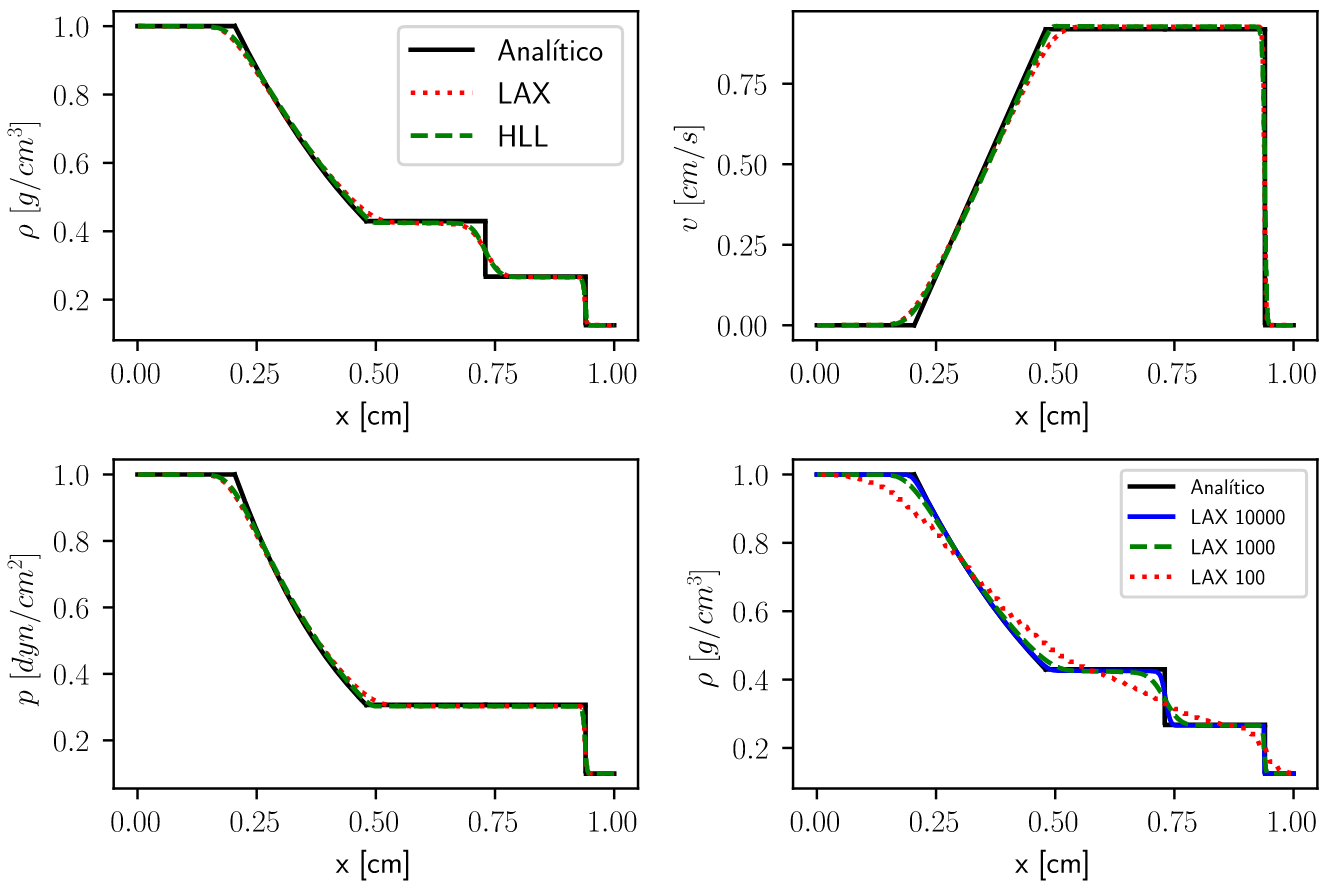
\includegraphics[width=1.0\textwidth]{./Figuras/verificacion_del_codigo/rarefaction.png}
  \caption{Representación del caso 1 newtoniano a $t = 0.25$ s. Las magnitudes mostradas con
  la densidad (arriba a la izquierda), la velocidad (arriba a la derecha) y la presión (abajo a la 
  izquierda).
  El panel de abajo hacia la derecha muestra la comparación a distintas resoluciones para la densidad. Los demás páneles muestran
  las diferencias de los métodos HLL y Lax con una resolución de 10,000 píxeles.
  \label{comparacion_analitico_newtoniano_caso_1}}
\end{figure}

En el 2° caso newtoniano, se simulan 2 ondas de rarefacción, para este caso los valores de la 
densidad
y presión serán las mismas en ambos estados del tubo, pero las velocidades serán de igual magnitud
pero de sentido contrario. Por lo que una se moverá a la izquierda el otro a la derecha, como se 
puede ver en el cuadro \ref{Cuadro_parametros_sod_tube}.
La Figura \ref{caso_new_rar_rar} muestra, usando
el método de Lax, la evolución temporal del 2° caso newtoniano. El panel de arriba a la izquierda muestra la densidad.
El panel arriba a la derecha muestra la velocidad y el de abajo, la presión.

\begin{figure}
  \centering
      \subfigure{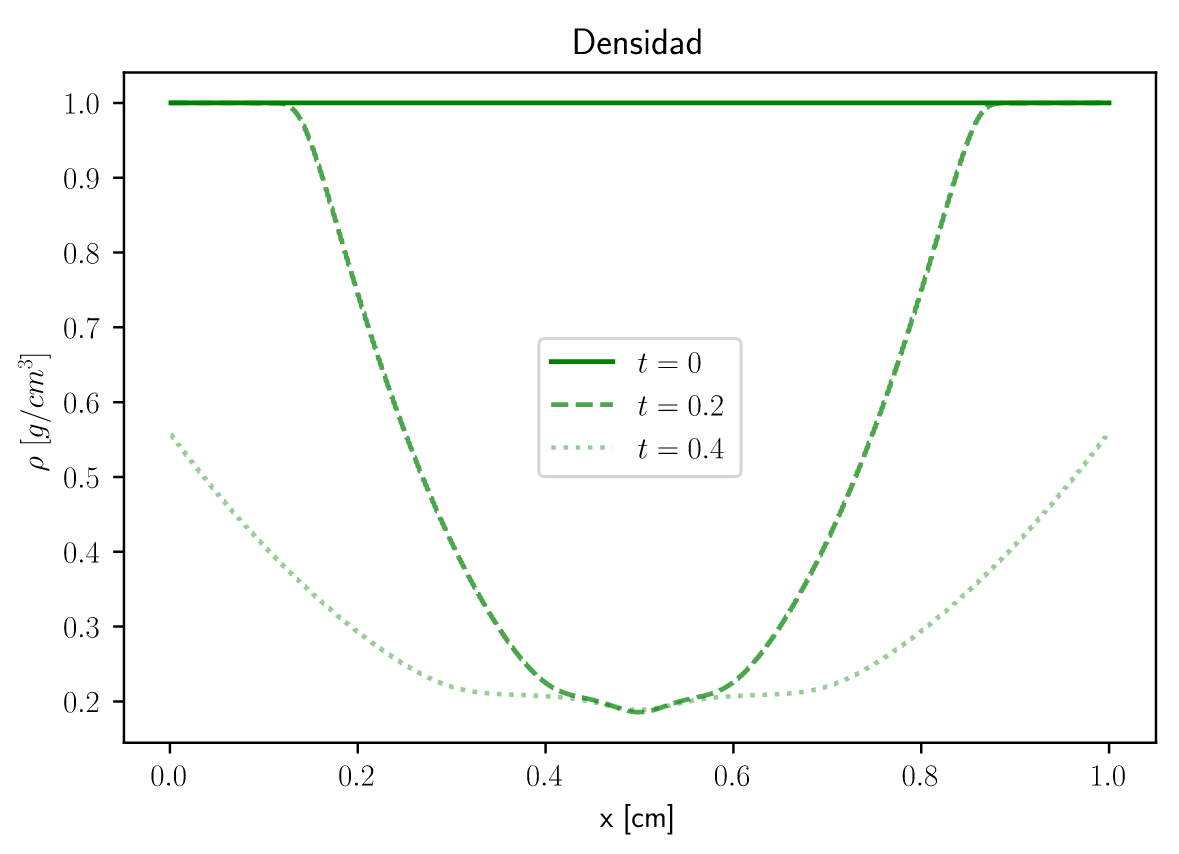
\includegraphics[scale = 0.16]{./Figuras/verificacion_del_codigo/caso_newtoniano/caso_new_rar_rar_rho.png}}
      \subfigure{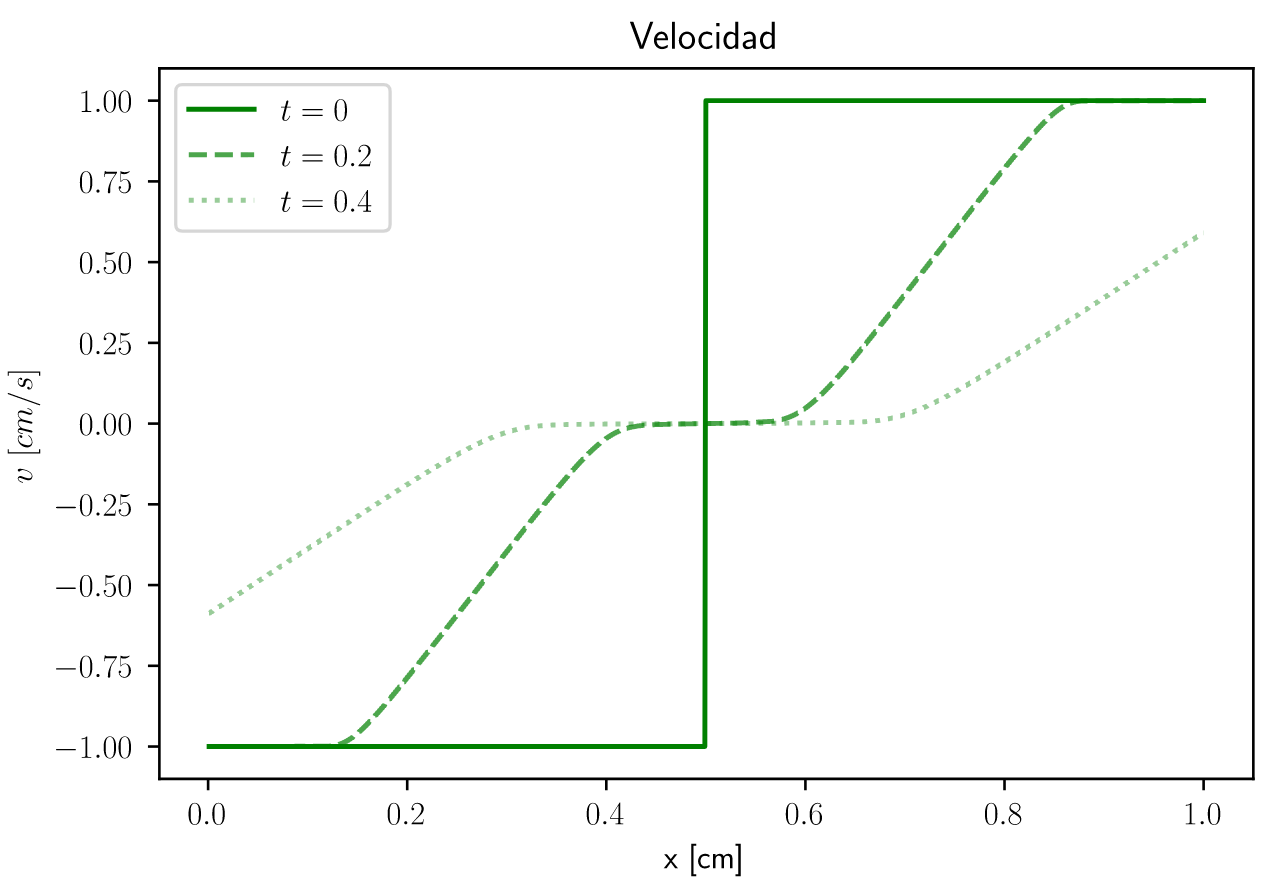
\includegraphics[scale = 0.16]{./Figuras/verificacion_del_codigo/caso_newtoniano/caso_new_rar_rar_v.png}}
      \subfigure{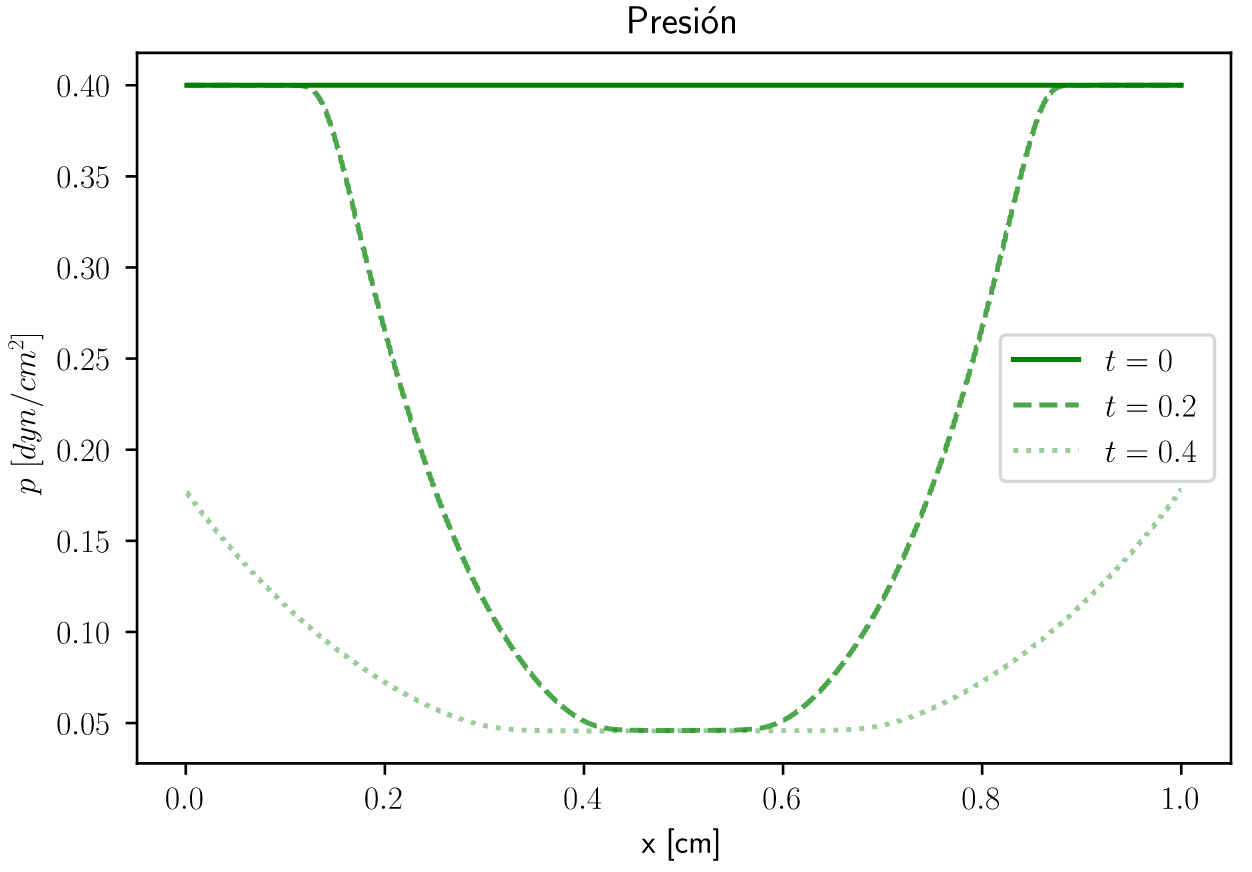
\includegraphics[scale = 0.16]{./Figuras/verificacion_del_codigo/caso_newtoniano/caso_new_rar_rar_p.png}}
    \caption{ Igual que en la Figura \ref{caso_new_rar_shock} pero para el caso 2 newtoniano. 
    El índice adiabático sigue siendo $\Gamma = 7/5$.
    \label{caso_new_rar_rar}.}
\end{figure}

Para los valores $t = 0$ s, la densidad ($\rho$) y la presión ($p$) son las mismas, 
mientras que para el panel de
la velocidad  tiene una discontinuidad en $x = 0.5$ cm. 
Para el tiempo $t = 0.2$ s, se puede ver una 
simetria ya que la cabeza de la onda de rarefacción tienen lugar en los puntos $x \approx 0.16$ cm
donde la densidad $\rho = 1.0 \,  \text{g}/ \text{cm}^3$ y 
la presión $p = 0.40 \,  \text{dyn}/ \text{cm}^2 $,
decrecen hasta $\rho \approx 0.25 \,  \text{g}/ \text{cm}^3$ y $p = 0.05 \,  \text{dyn}/ \text{cm}^2 $ en forma parabólica hasta conectar con la cola de 
la onda de rarefacción, mientras que la velocidad $v = -1.0 $ cm/s decrece linealmente en magnitud 
hasta $v = 0$ cm/s. Entre los puntos $x \approx 0.4$ cm y $x \approx 0.6$ cm, que es la zona de contacto, mantienen
un valor constante para conectar con la cola de la onda de rarefacción donde la densidad y presión 
crecen parabólicamente hasta $x \approx 0.84$ cm, mientras que la velocidad lo hace linealmente al mismo puntos.
Esa región es la cabeza de la onda y conecta con los estados iniciales del lado derecho del tubo, 
donde no ha habido perturbación, y por ende, $\rho = 1.0 \,  \text{g}/ \text{cm}^3$, 
$v = 1$ y $p = 0.4 \,  \text{dyn}/ \text{cm}^2 $.

Para el tiempo $t = 0.4$ s se aprecian las colas de las ondas de rarefacción
en los puntos $x  \approx 0.3$ y $x  \approx 0.7$, donde la densidad mantiene un valor contante 
$\rho \approx 0.25 \,  \text{g}/ \text{cm}^3$, la velocidad $v \approx 0.0$ cm/s y la presión $p = 0.05 \,  \text{dyn}/ \text{cm}^2 $.

La comparación del método de Lax y HLL se da en la Figura \ref{comparacion_analitico_newtoniano_caso_2}.
Como se puede ver en los páneles de densidad (arriba a la izquierda) en el punto $x \lesssim  0.05$ cm,
la densidad no esta perturbada y tiene un valor $\rho = 1.0 \,  \text{g}/ \text{cm}^3$,
la velocidad (arriba a la derecha)
$v = -1.0$ cm/s y la presión (abajo a la izquierda) $p = 0.4 \,  \text{dyn}/ \text{cm}^2 $. Tanto Lax como HLL se ajustan perfectamente 
para valores constantes. Despues del punto de la cabeza de la onda los valores de la densidad y 
la presión empiezan a dsiminuir a $\rho \approx 0.2 \,  \text{g}/ \text{cm}^3$ y $p \approx 0.05 \,  \text{dyn}/ \text{cm}^2 $
en forma parabólica, mientras que la velocidad disminuye (en magnitud) linealmente hasta $v = 0$ cm/s.
Cabe señalar que los valores más bajos a los que disminuyen las magnitudes de densidad, velocidad y 
presión son en el punto $x \approx 0.33$ cm, el cual es la cola de la onda de rarefacción. Al comparar
las resoluciones, se nota que para resoluciones $\leq 1,000$ no se apega al método analítico sobre 
todo en la cabeza de la onda.

De $x \approx 0.33$ cm , la densidad, velocidad y presión 
mantienen valores constantes de $\rho \approx 0.1 \,  \text{g}/ \text{cm}^3$, $v \approx 0$ cm/s y 
$p = 0.05 \,  \text{dyn}/ \text{cm}^2 $ 
hasta llegar al punto $x \approx 0.66$ cm donde conectan con la cola de la onda de rarefacción. En
esta región donde se enlazan las colas de la onda Lax no tiene problemas con ningúnn tipo de resolución.
Del punto de la cola de la onda de rarefacción de la derecha, la densidad y presión empiezan a subir 
sus valores en forma parabólica hasta a $\rho  =  1.0$ y a $p = 0.4 \,  \text{dyn}/ \text{cm}^2 $, 
mientras la velocidad incrementa
linealmente a a $v = 1.0$ cm/s. El punto final hasta donde incrementan sus valores es la cabeza de la onda 
de rarefacción derecha el cual es $ x \approx 0.93 $ cm.
{\color{red} En el panel de abajo a la derecha muestra la solución analítica, así como los resultados obtenidos 
usando Lax\footnote{
  Se usó el método de Lax ya que es más rápido que HLL
}
con distintas resoluciones ($nx = 10^2, \, 10^3, \,10^4$). Al igual que el caso 1 newtoniano,
conforme se incrementa la resolución, los resultados numéricos se apegan más a la solución analítica.
A partir de resoluciones mayores a 1000 los resultados se apegan mucho a la solución analítica.}



Notamos que para resoluciones $\leq 1000$ Lax no se ajusta correctamente debido al cambio de valor 
en $x \approx 0.05$ cm donde inicia la cabeza de la onda de rarefacción. Para los puntos 
$x \gtrsim 0.93$ cm, los valores de la densidad, presión y velocidad se mantienen en 
$\rho = 1 \,  \text{g}/ \text{cm}^3$, 
$p = 0.4 \,  \text{dyn}/ \text{cm}^2 $ y $v = 1.0$ cm/s, es decir, no han sido perturbados por la onda. Debido 
a la cabeza de la onda Lax no se ajusta bien al método analítico para resoluciones $\leq 100$ píxeles.
Para el panel de abajo a la derecha, mientras no haya discontinuidades de salto
como en el anterior caso ambos procedimientos funcionan para resoluciones $\leq 100$ píxeles.


\begin{figure}
  \centering
    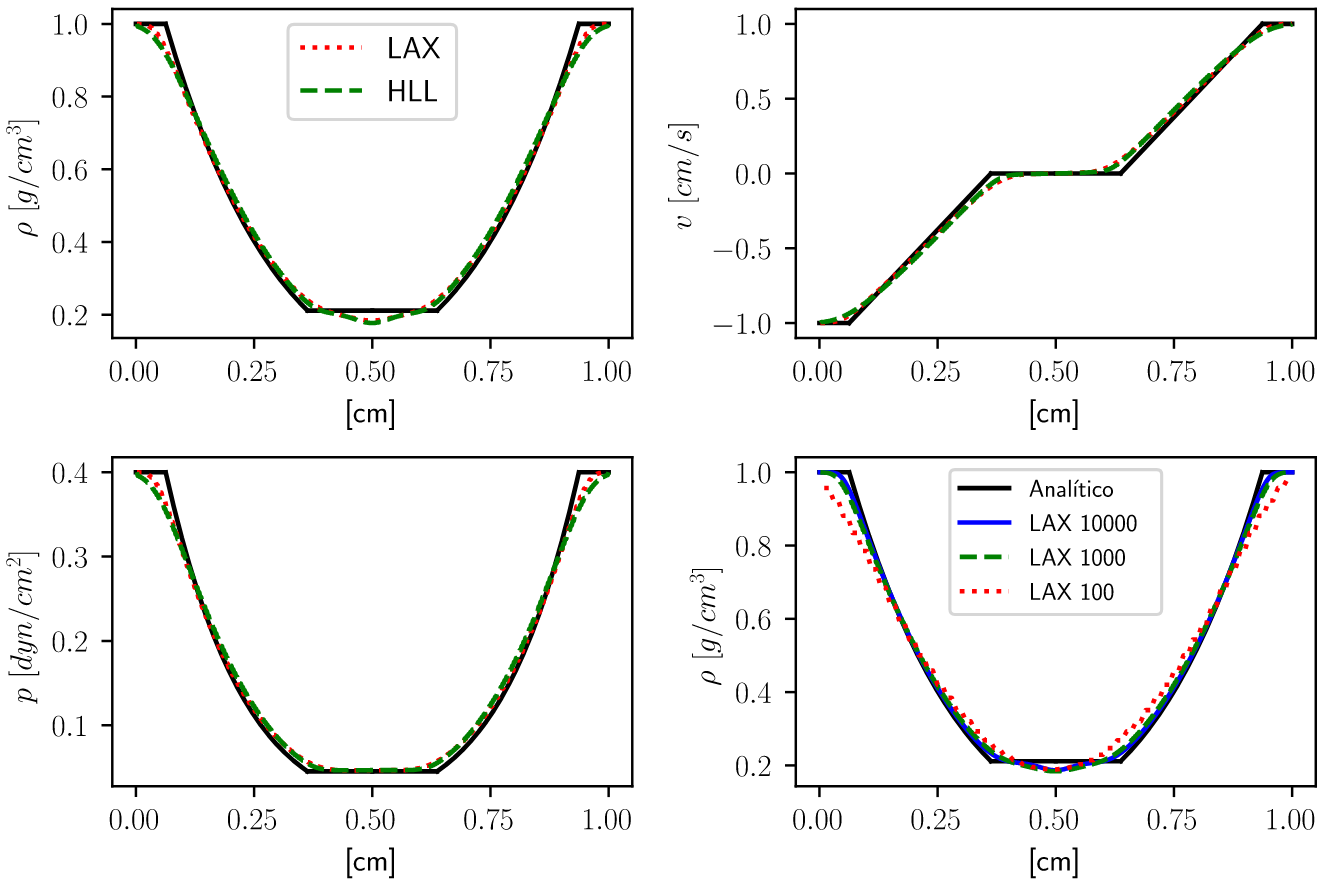
\includegraphics[width=1.0\textwidth]{./Figuras/verificacion_del_codigo/rarefaction-rarefaction.png}
  \caption{ Igual que en la Figura \ref{comparacion_analitico_newtoniano_caso_1} pero para el caso 2 newtoniano.
    a $t = 0.25$ s. Los páneles vienen en 
  el mismo orden que la figura.
  El panel de abajo hacia la derecha muestra la comparación a distintas resoluciones para la densidad. 
  Los demás páneles muestran las diferencias de los métodos HLL y Lax con una resolución 
  de 10,000 píxeles.
  \label{comparacion_analitico_newtoniano_caso_2}} 
\end{figure}

% Para los casos newtonianos se pueden usar Lax o HLL ya que ambos se ajustan con el método analítico
% (Lora-Clavijo \emph{et. al.} 2013)
% y con una resolución $\leq 1000$ píxeles.

Podemos concluir, para el caso newtoniano, que nuestros módulos de 
Lax como HLL reproducen de forma casi perfecta la solución analítica para este 
problema de Riemann
(Lora Clavijo \emph{et al.} 2013), ya sea en las regiones donde se muestra una discontinuidad
o donde cambia suavemente. 
Cabe destacar que el método Lax resultó ser 220 \% más rápido que HLL. 
\footnote{Probado con una resolución de 10,000 píxeles con un procesador AMD Ryzen 3 3300U de
2.10 Ghz} 
.

% ========================================================================================================
% ========================================================================================================


\subsection{Casos relativistas}

Para los casos relativistas, se tomarán valores a partir de los cuales $v \rightarrow c$,
y además se requiera usar el índice adiabático\footnote{En esta tesis,
para fines explícitos, se tomará gamma mayúscula ($\Gamma$) como el índice adiabático. Mientras que 
gamma minúscula ($\gamma$) como el factor de Lorentz.} $\Gamma = 4/3$. Los valores con los que se 
toman los casos del caso relativista estan en el cuadro \ref{Cuadro_parametros_sod_tube_rel} y 
cabe señalar que la velocidad de la luz está normalizada a $c = 1$.

\begin{table}[htbp]
  \begin{center}
  \begin{tabular}{|c|c|c|c|c|c|c|}
  \hline 
  \textbf{Caso} & \textbf{$p_l$} [$\text{dyn}/\text{cm}^2$] & \textbf{$p_r$} [$\text{dyn}/\text{cm}^2$] & \textbf{$v_l$}/c & \textbf{$v_r$}/c  & \textbf{$\rho_l$} [$\text{g}/\text{cm}^3$]& \textbf{$\rho_r$} [$\text{g}/\text{cm}^3$]\\ 
  \hline 
  Caso 1 & 13.33  & 0.0  & 0.0 & 0.0 & 10  & 1 \\ 
  \hline 
  Caso 2 & 0.05  & 0.05  & -0.2 & 0.2 & 0.1  & 0.1  \\ 
  \hline 
  \end{tabular}
  \caption{\label{Cuadro_parametros_sod_tube_rel} Valores iniciales 
  de la presión ($p$), velocidad ($v$)
  y densidad ($\rho$), del lado izquierdo ($p_l, v_l, \rho_l$) y derecho ($p_r, v_r, \rho_r$)
  para los casos relativistas. Para todos los
  casos el dominio espacial será $x \in [0,1]$, la 
  posición crítica será $x_0 = 0.5$ y un índice adiabático $\Gamma = 4/3$}
  \end{center}
\end{table}

Tanto en el caso 1 relativista como el caso 2 relativista, la evolución temporal se hará usando 
el método de HLL ya que Lax falla al tratar de simular las condiciones iniciales de este problema. 
Además de que necesita de altas resoluciones $\geq 10,000$ píxeles para poder funcionar.

\begin{figure}
  \centering
      \subfigure{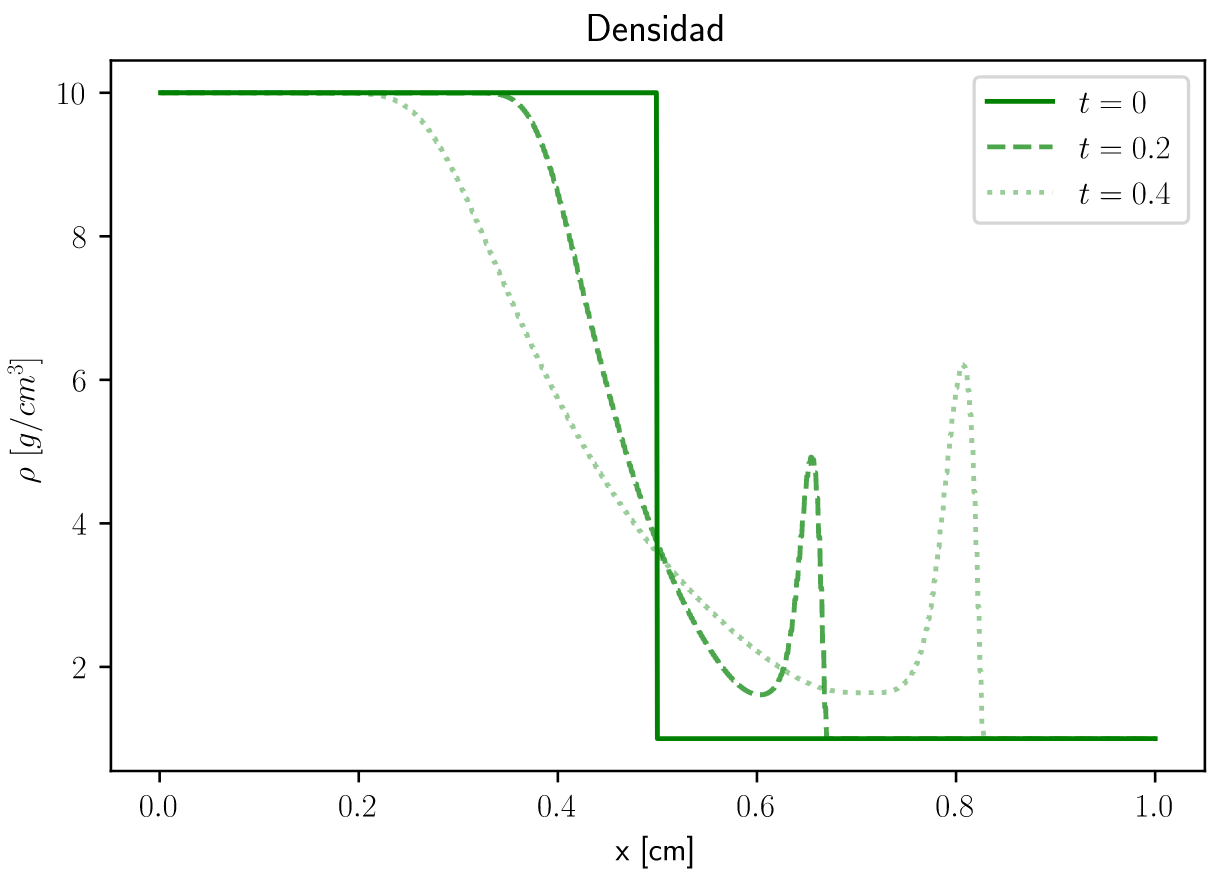
\includegraphics[scale = 0.16]{./Figuras/verificacion_del_codigo/caso_relativista/caso_rel_rar_shock_rho.png}}
      \subfigure{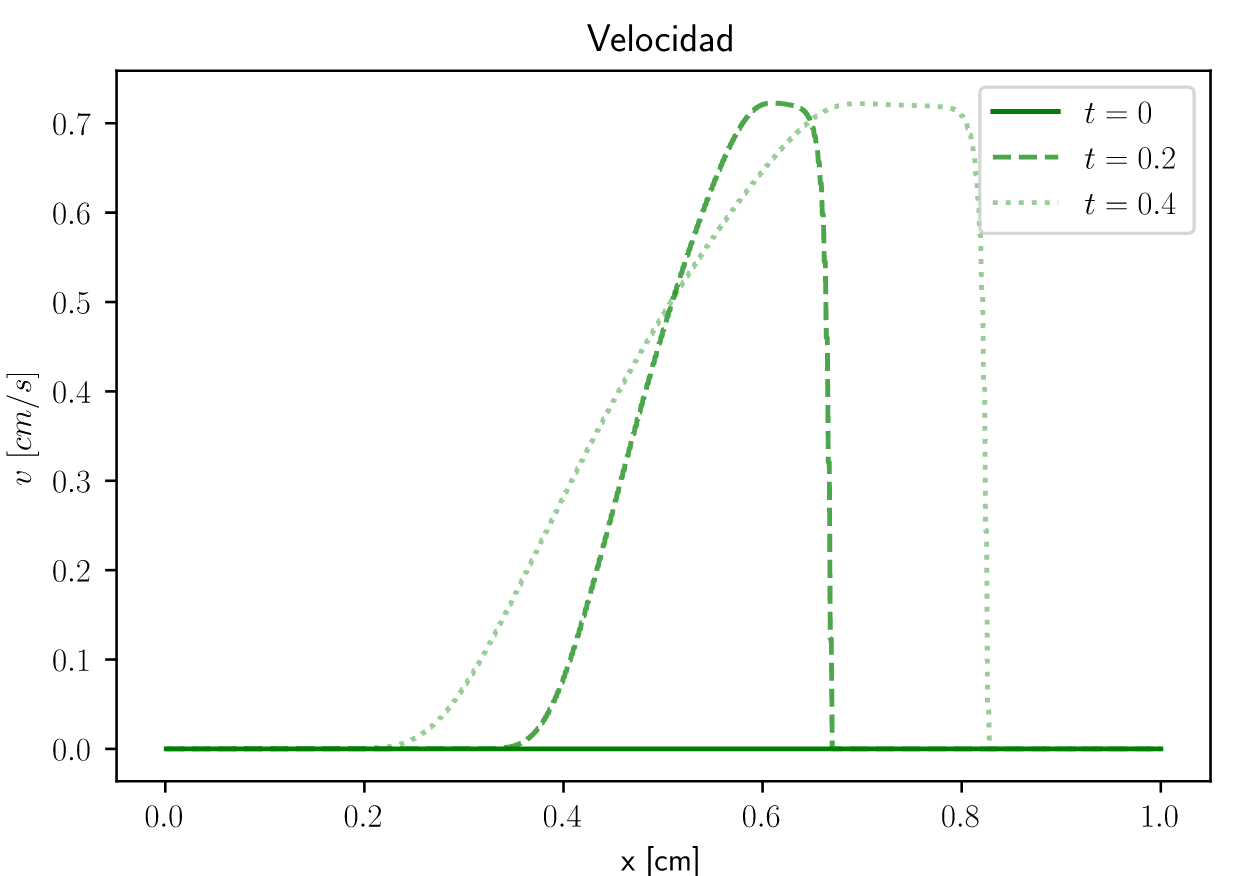
\includegraphics[scale = 0.16]{./Figuras/verificacion_del_codigo/caso_relativista/caso_rel_rar_shock_v.png}}
      \subfigure{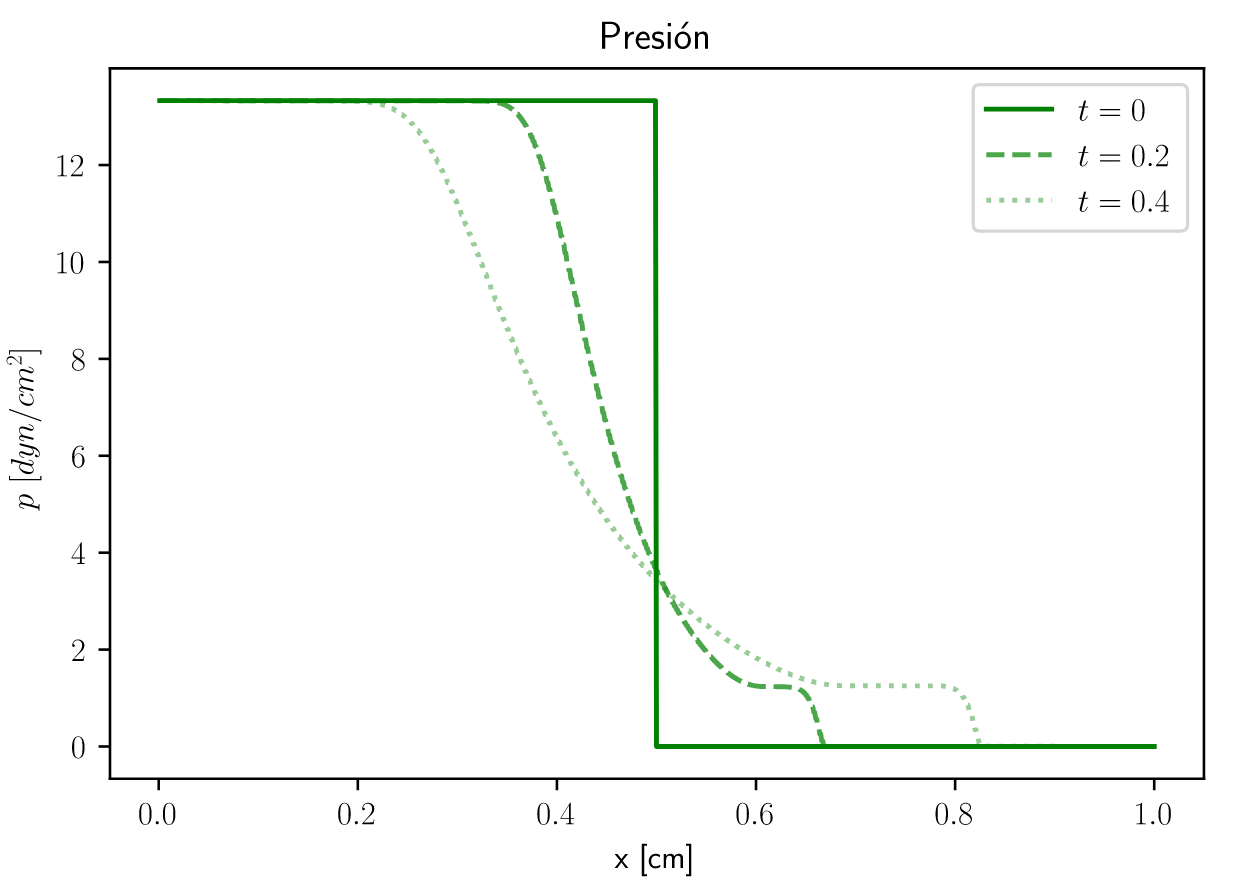
\includegraphics[scale = 0.16]{./Figuras/verificacion_del_codigo/caso_relativista/caso_rel_rar_shock_p.png}}
    \caption{Igual que en la Figura \ref{caso_new_rar_shock} pero para el caso 1 relativista. A diferencia 
    del caso newtoniano, en el relativista se usa un índice adiabático $\Gamma = 4/3$. \label{caso_rel_rar_shock_1}}
\end{figure}

En la Figura \ref{caso_rel_rar_shock} cuando $t = 0$ s el panel de la densidad (arriba a la izquierda) 
y presión (abajo ) presentan una discontinuidad en $x = 0.5$ cm donde $\rho = 10 \,  \text{g}/ \text{cm}^3$
y $p = 13.33 \,  \text{dyn}/ \text{cm}^2 $ del lado izquierdo, mientras que del lado derecho $\rho = 0  \,  \text{g}/ \text{cm}^3$
y $p = 0 \,  \text{dyn}/ \text{cm}^2 $. La velocidad no presenta discontinuidad y mantiene su velocidad nula para toda
la región del tubo. 

Al tiempo $t =0.2$ s la densidad y presión 
descienden linealmente, mientras que la velocidad asciende en $x = 0.42$ cm
que viene siendo la cabeza de la onda de rarefacción. El punto donde alcanzan 
sus máximos y minimos es la cola de la onda que esta situada en el punto $x \approx 0.58$ cm,
le densidad y presión llegan a $\rho \approx 1.12 \,  \text{g}/ \text{cm}^3$ y 
$p \approx 1.12\,  \text{dyn}/ \text{cm}^2 $ mientras que las velocidad es
cercana a la de la luz $v \approx 0.75c$. Las densidad vuelve a subir en el punto $x \approx 0.63$ cm
y llega a $\rho = 5.6  \,  \text{g}/ \text{cm}^3$ mientras que la velocidad y presión se mantienen iguales. Para el punto
$x \approx 0.68$ cm, la densidad, presión y velocidad bajan a valores nulos que es la zona del tubo que
no ha sido perturbada por la onda.

Para el tiempo $t = 0.4$ s, la densidad y presión, que mantienen sus valores de 
$\rho = 10 \,  \text{g}/ \text{cm}^3$ y 
$p = 13.33 \,  \text{dyn}/ \text{cm}^2 $ bajan sus valores en $x \approx 0.25$ cm, mientras que la velocidad , la cual es nula,
asciende. En el punto $x \approx 0.68$ cm la presión alcanza $p \approx 1.12\,  \text{dyn}/ \text{cm}^2 $ y la densidad
$\rho \approx 1.12 \,  \text{g}/ \text{cm}^3$, mientras que la velocidad sube a $v \approx 0.75c$. 
La densidad vuelve a subir
en $x \approx 0.75$ cm y llega a $\rho \approx 0.65 \,  \text{g}/ \text{cm}^3$ y 
se mantiene así hasta el punto $x \approx 0.83$ cm
donde la densidad, así como la velocidad y presión descienden sus valores a nulos.

En la Figura \ref{caso_rel_rar_shock} el panel de arriba a la izquierda muestra la densidad, el de 
arriba a la derecha la velocidad, la presión es el de abajo a la izquierda. Cabe recalcar que  el tiempo 
fue a $t = 0.35$ s.

A la región $x \lesssim 0.33$ cm, la densidad tiene un valor $\rho = 10 \,  \text{g}/ \text{cm}^3$, 
la presión $p = 13.33 \,  \text{dyn}/ \text{cm}^2 $
y la velocidad es nula se puede ver que HLL se ajusta perfectamente para los valores constantes
sin importar la resolución. 
En el punto $x \approx 0.33$ cm se localiza la cabeza de la onda donde la presión y la densidad 
empiezan a decaer en forma parabólica, mientras que que la velocidad comienza subir en forma linealmente.
El punto donde la densidad y presión alcanzan su mínimo y la velocidad su máximo es la cola de la onda 
de rarefacción y se localiza en $x \approx 0.62$ cm. La resolución para esta región es $\geq 500$ 
píxeles. En el punto $x \approx 0.75$ cm únicamente 
la densidad tiene una discontinuidad, al cual se le conoce como discontinuidad de la onda de contacto
debido a esta región la resolución a tomar en cuenta debe ser $\geq 1,000$ o incluso $\geq 10,000$.
En esta discontinuidad la densidad pasa de $ \rho \approx 3 \,  \text{g}/ \text{cm}^3$ a
$ \rho \approx 9 \,  \text{g}/ \text{cm}^3$ mientras que la presión 
y velocidad se mantienen en $p \approx 2\,  \text{dyn}/ \text{cm}^2 $ 
y $v = 0.75$ c. La última discontinuidad que es la de choque,
todas las magnitudes ($\rho$, $v$ y $p$) disminuyen a su valor nulo y la resolución a tomar en cuenta
puede ser $\geq 1,000$ píxeles dado que HLL no presenta dificultades con esta discontinuidad.

{\color{red}En el panel de abajo a la derecha muestra la solución analítica, así como los resultados obtenidos 
usando HLL con distintas resoluciones ($nx = 10^2, \, 10^3, \,10^4$).  
En específico, para el problema 1 relativista, a partir de resoluciones mayores a 1000 los
resultados se apegan mucho a la solución analítica.}

En el panel de velocidad de la Figura \ref{caso_rel_rar_shock} podemos ver que HLL no tiene problemas 
al compararse con el método analítico, cuando este alcanza velocidades cercanas a la de la luz.

\begin{figure}
  \centering
    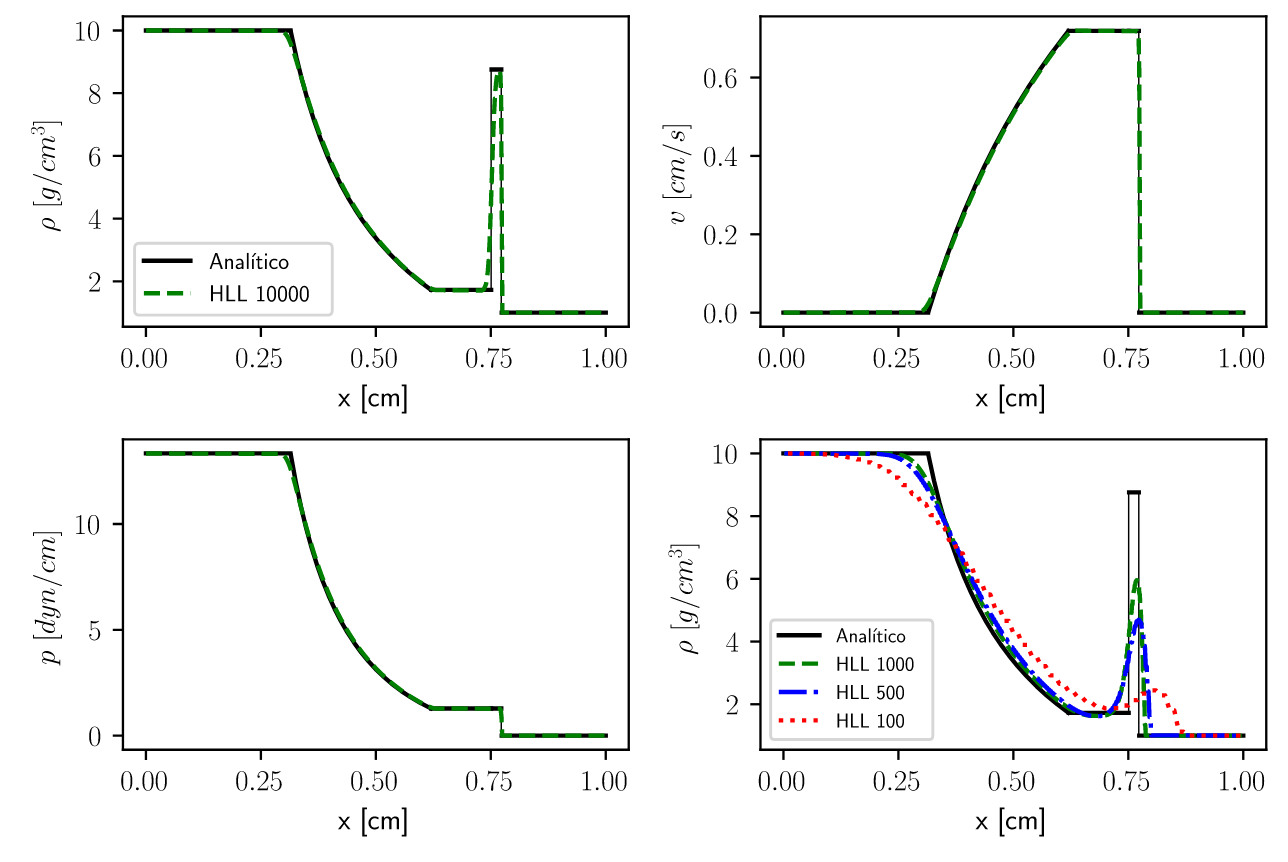
\includegraphics[width=1.0\textwidth]{./Figuras/verificacion_del_codigo/caso_relativista/caso_rel_rar_shock.png}
  \caption{Igual que en la Figura \ref{comparacion_analitico_newtoniano_caso_1} pero para el caso 1 
  relativista 
  a $t = 0.35$ s. El panel de abajo 
  hacia la
  derecha muestra la comparación a distintas resoluciones para la densidad. Los demás páneles muestran
  las diferencias de los métodos HLL y Lax con una resolución de 10,000.}\label{caso_rel_rar_shock}
\end{figure}

El caso 2 relativista representa 2 ondas de rarefacción, a diferencia del caso 1 las velocidades que 
alcanzan las 
ondas no son velocidades relativistas.
\begin{figure}
  \centering
      \subfigure{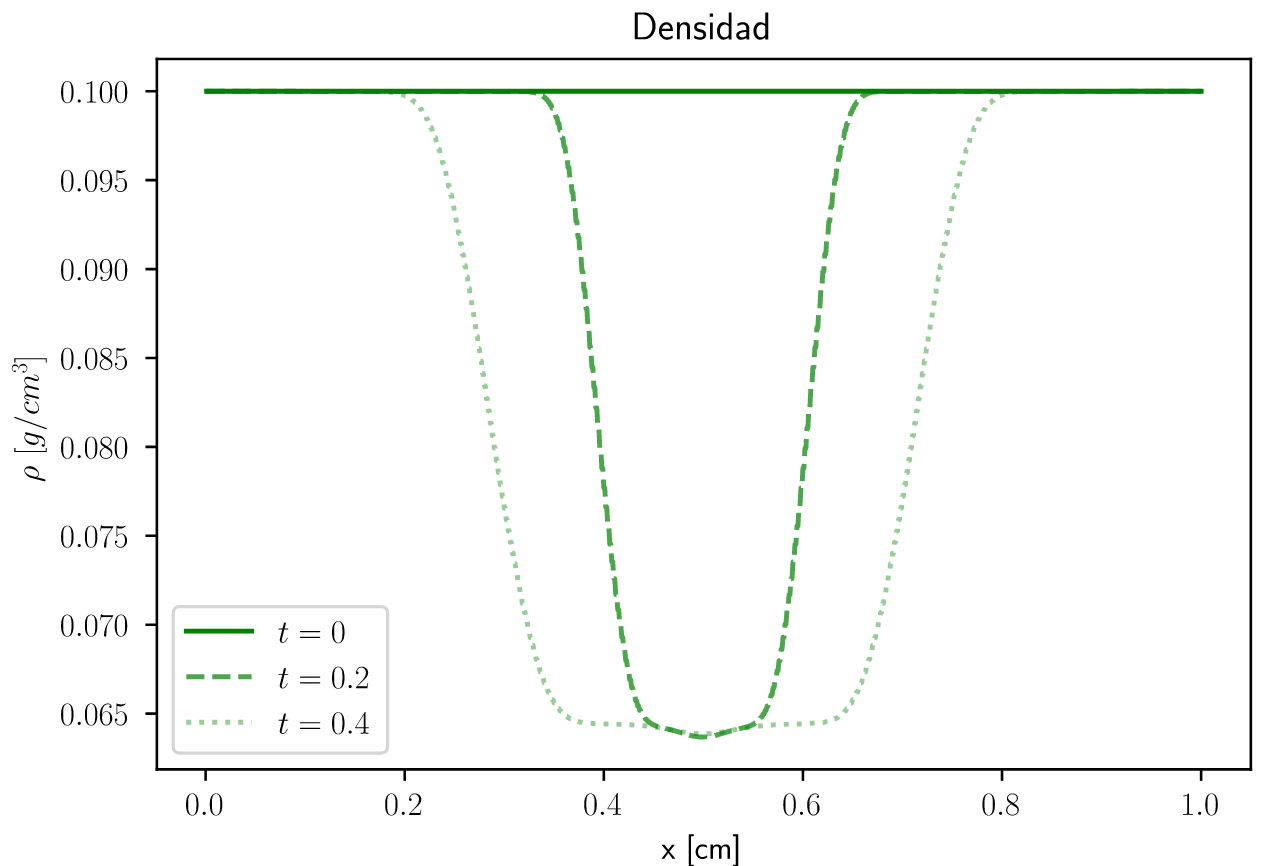
\includegraphics[scale = 0.16]{./Figuras/verificacion_del_codigo/caso_relativista/caso_rel_rar_rar_rho.png}}
      \subfigure{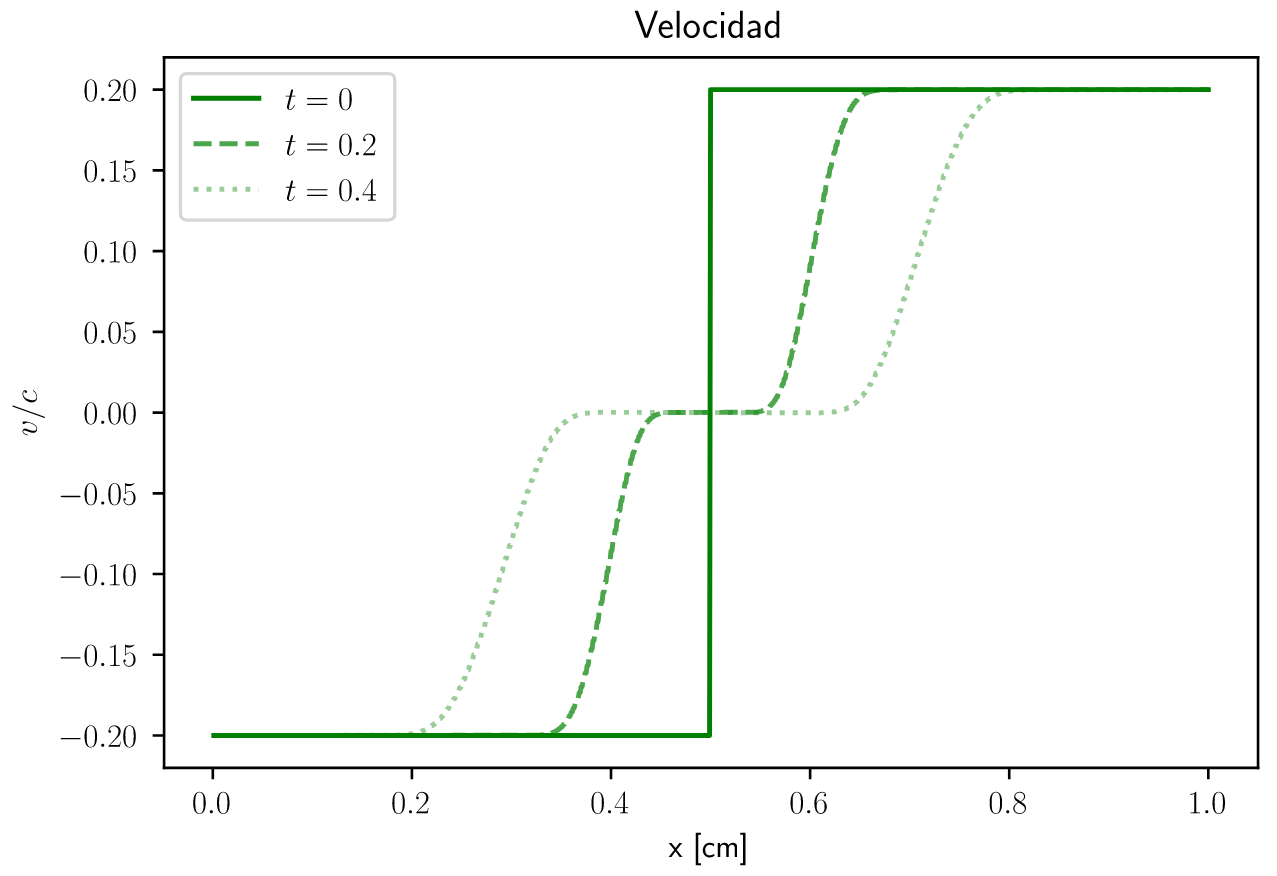
\includegraphics[scale = 0.16]{./Figuras/verificacion_del_codigo/caso_relativista/caso_rel_rar_rar_v.png}}
      \subfigure{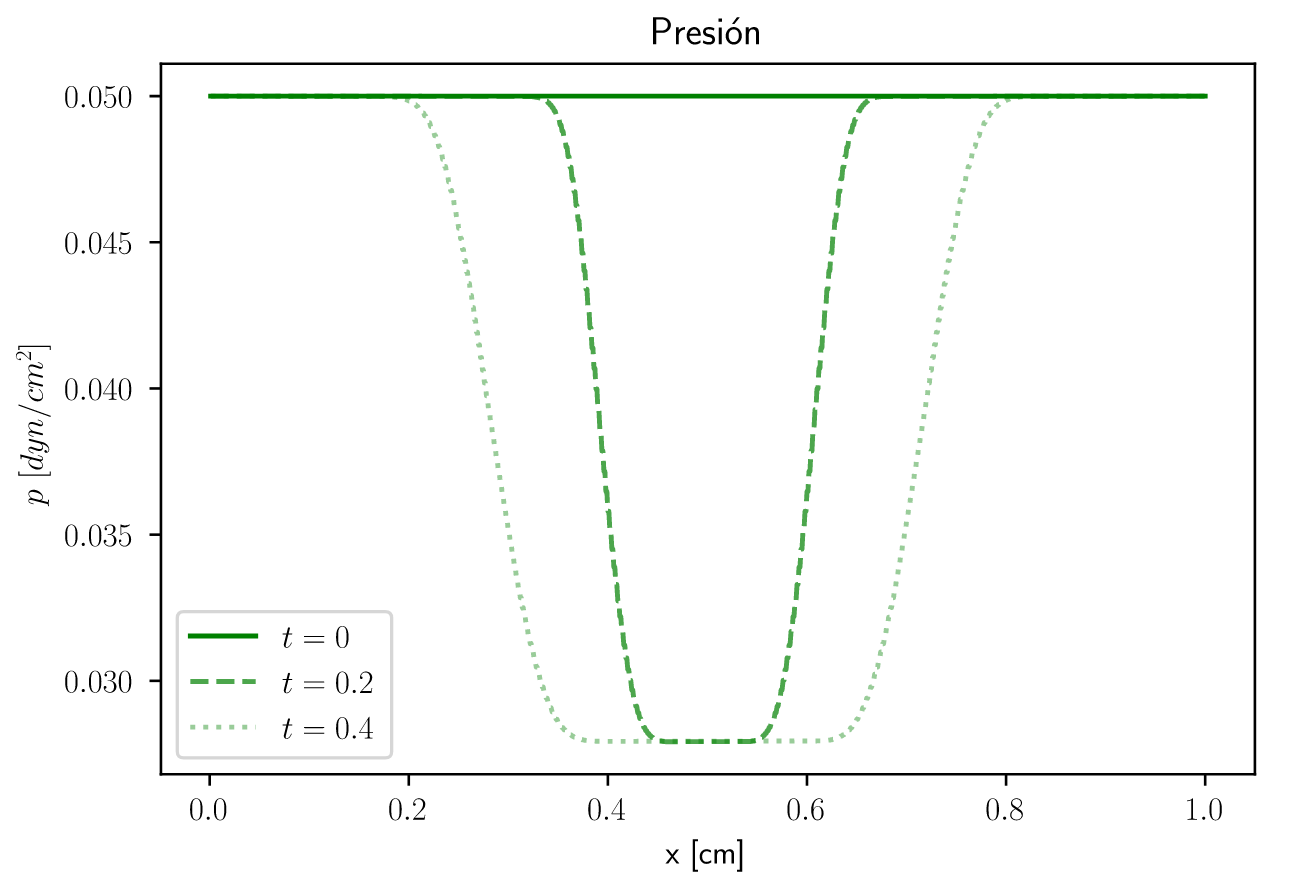
\includegraphics[scale = 0.16]{./Figuras/verificacion_del_codigo/caso_relativista/caso_rel_rar_rar_p.png}}
    \caption{Igual que en la Figura \ref{caso_new_rar_shock} pero para el caso 2 relativista. 
    El panel de arriba a la izquierda muestra la densidad.
    El de arriba a la derecha la velocidad y el de abajo la presión}\label{caso_rel_rar_shock_2}
\end{figure}

A diferencia del caso 1 relativista, el caso 2 relativista no presenta discontinuidades,
por lo que se pueden usar resoluciones $\leq 100.$ píxeles. En la Figura 
\ref{caso_rel_rar_shock_2},  
el panel de arriba a la izquierda muestra la densidad, el de arriba a la derecha la velocidad
y el de abajo la presión.
Al igual que el caso newtoniano al simular las 2 ondas presenta una simetría con respecto a la 
discontinuidad.
En el tiempo $t = 0$ s, tanto la densidad como la presión mantienen los mismos valores 
$\rho =0.1 \,  \text{g}/ \text{cm}^3$
y $p = 0.05$. mientras que la velocidad tiene una discontinuidad en $x = 0.5$ cm donde la parte del lado
izquierdo de la discontinuidad es $v = -0.2$ c, mientras que del lado derecho es $v = 0.2$ c.

Al tiempo $t = 0.2$ s la cabeza de la onda de rarefacción se presenta en los punto 
$x \approx 0.35$ cm donde los valores de de la presión ($p = 0.05$) y densidad 
($\rho =0.1 \,  \text{g}/ \text{cm}^3$) comienzan a descender linealmente,
mientras que la velocidad ($v = 0.2$ c) desciende, solo en magnitud, hasta el punto $x \approx 0.45$ cm
que viene siendo la cola de la onda. En este punto los valores de la densidad, presión y velocidad
son $\rho \approx 0.065 \,  \text{g}/ \text{cm}^3$, $p \approx 0.028\,  \text{dyn}/ \text{cm}^2 $ 
y $v \approx 0$ c. Los valores cambian en 
$ x \approx 0.55$ cm
que es la cola de la onda de rarefacción derecha, y comienzan a subir
hasta $x \approx 0.65$ cm donde ahora la densidad es 
$\rho = 0.1 \,  \text{g}/ \text{cm}^3$, la presión $p = 0.05 \,  \text{dyn}/ \text{cm}^2 $ y 
la velocidad $v = 0.2$ c

Para el tiempo $t = 0.4$ s se sigue manteniendo el mismo sistema que al tiempo $t =0.2$ s, ya que en
$x \approx 0.25$ cm los valores de la densidad ($\rho = 0.1 \,  \text{g}/ \text{cm}^3$), 
presión ($p = 0.05 \,  \text{dyn}/ \text{cm}^2 $) 
y velocidad ($v = -0.2$ c) descienden en forma lineal hasta el punto $x \approx 0.35$ cm, donde 
se mantienen constantes los valores ($\rho \approx 0.065  \,  \text{g}/ \text{cm}^3$, 
$p \approx 0.028\,  \text{dyn}/ \text{cm}^2 $ y $v \approx 0$ c) 
hasta el punto $x \approx 0.65$ cm donde vuelven a ascender linealmente
hasta el punto $x = 0.75$ cm donde los valores regresan a $\rho = 0.1 \,  \text{g}/ \text{cm}^3$, 
$p = 0.05 \,  \text{dyn}/ \text{cm}^2 $ y la velocidad 
cambia de sentido $v = 0.2$ c.


\begin{figure}
  \centering
    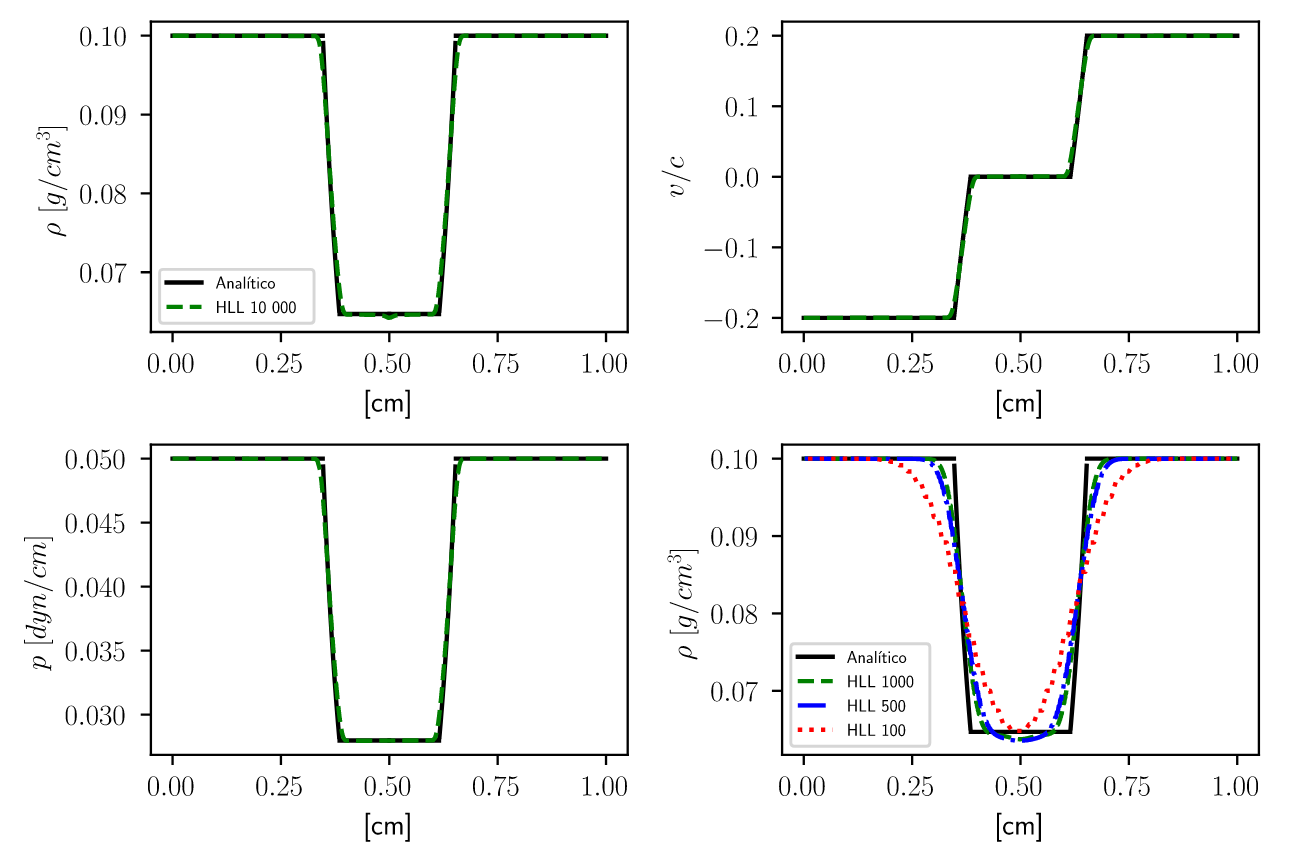
\includegraphics[width=1.0\textwidth]{./Figuras/verificacion_del_codigo/caso_relativista/caso_rel_rar_rar.png}
  \caption{Igual que en la Figura \ref{comparacion_analitico_newtoniano_caso_1} pero para el caso 2 
  relativista. Se usó un índice adiabático $\Gamma = 4/3$ y $t = 0.25$ s.
  } \label{caso_rel_rar_shock_2}
\end{figure}

En la Figura \ref{caso_rel_rar_shock_2}, el panel de arriba a la izquierda muestra el perfil de la 
densidad, el de arriba a la derecha la velocidad, el de abajo a la izquierda la presión. Esos 3 muestran
na comparación entre el método analítico y el método numérico (HLL) usando una resolución de 
10,000 píxeles. 

En $x \lesssim 0.33$ cm los valores de de la densidad, presión y velocidad son 
$\rho = 0.1 \,  \text{g}/ \text{cm}^3$, $p = 0.05 \,  \text{dyn}/ \text{cm}^2 $
y $v = -0.2$ c. HLL para resoluciones $\geq 500$ se ajusta perfectamente al analítico. Cuando los 
valores descienden en $x \approx 0.37$ cm a $\rho \approx 0.075 \,  \text{g}/ \text{cm}^3$, 
$v \approx 0$ c y $p \approx 0.025\,  \text{dyn}/ \text{cm}^2 $. En
esta región podemos ver que para resoluciones $\leq 100$ pixeles se tiene dificultades para apegarse al
método analítico sobre todo en las regiones de la cabeza y cola de la onda de rarefacción, donde suaviza
esos puntos. En el punto $x \approx 0.63$  cm tanto la presión como la densidad y la velocidad vuelven a subir
sus valores hasta el punto $x \approx 0.65$ cm donde alcanzan los valores que tenial del lado izquierdo
donde la densidad ahora es $\rho = 0.1 \,  \text{g}/ \text{cm}^3$, la presión $p = 0.05 \,  \text{dyn}/ \text{cm}^2 $ 
y la velocidad $v = 0.2$ c.
{\color{red}En el panel de abajo a la derecha muestra la solución analítica, así como los resultados obtenidos 
usando HLL con distintas resoluciones ($nx = 10^2, \, 10^3, \,10^4$). 
Al igual que el caso 1 relativista,
conforme se incrementa la resolución, los resultados numéricos se apegan más a la solución analítica.
A partir de resoluciones mayores a 1000 los resultados se apegan mucho a la solución analítica.}

% El módulo de HLL se apega a la analítica, para los puntos en $x \approx 0.63$ cm y $x \approx 0.65$ cm para 
% resoluciones $ \geq 500$ ya que, para resoluciones menores, se 
% suavizan demasiado las colas y cabezas de las ondas de rarefacción. 
Por lo tanto podemos concluir que nuestro módulo HLL se ajusta perfectamente para el problema de 
Riemann relativista con resoluciones $\geq 500$ píxeles.

% ===============================================================================================
% ===============================================================================================


\section{Pruebas bidimensionales}
Ya que hemos visto el código funcionar correctamente para pruebas en una dimensión ahora nos toca ver
como funciona en 2 dimensiones. Se hará una prueba de una onda de choque relativista
en 2 dimensiones, los valores
que tendrá están en el cuadro \ref{Cuadro_parametros_choque_2D}.

\begin{table}[htbp]
  \begin{center}
  \begin{tabular}{|c|c|c|c|c|c|c|c|c|}
  \hline 
  \textbf{Caso} & \textbf{$p_i$} [$\text{dyn}/\text{cm}^2$] & 
  \textbf{$p_o$} [$\text{dyn}/\text{cm}^2$] & 
  \textbf{$v_{xi}$}/c & \textbf{$v_{xo}$}/c  & \textbf{$v_{yi}$}/c & \textbf{$v_{yo}$}/c  & 
  \textbf{$\rho_i$} [$\text{g}/\text{cm}^3$]& 
  \textbf{$\rho_o$} [$\text{g}/\text{cm}^3$]\\ 
  \hline 
  Caso 1 & 13.33  & 0.0  & 0.0 & 0.0 & 0.0 & 0.0 & 10  & 1 \\ 
  \hline 
  \end{tabular}
  \caption{\label{Cuadro_parametros_choque_2D} Valores iniciales 
  de la presión ($p$), velocidad ($v$)
  y densidad ($\rho$), del lado interno ($p_i, v_{x_{i}}, vy_i, \rho_i$) y 
  externo ($p_o, v_{xo}, v_{yo}, \rho_o$) de la onda de choque
  para los casos relativistas. Para todos los
  casos el dominio espacial será $x, y \in [0,1]\times[0,1] \, \text{cm}$, el radio de la onda
  será $r = 0.5 \, \text{cm}$ y un índice adiabático $\Gamma = 4/3$}
  \end{center}
\end{table}

Para comprobar que el código funciona correctamente en 2 dimensiones, se va a comparar
los perfiles de densidad, velocidad y presión de los radios de la onda de choque que son 
paralelos, perpendiculares y que forman un ángulo de 45° con el eje x con los resultados en 1 dimensión. 
La Figura \ref{Example_blast_wave} muestra una mejor representación visual de donde se tomarán los 
perfiles de la onda.

\begin{figure}
  \centering
    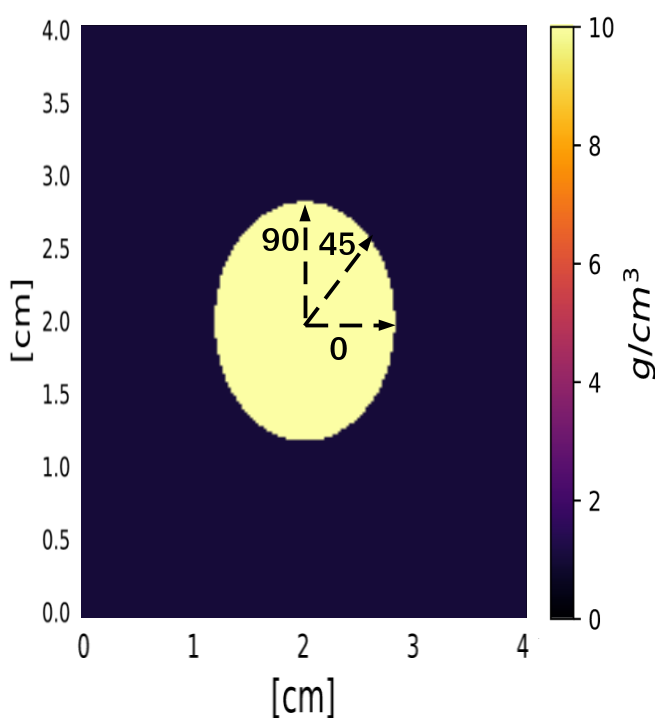
\includegraphics[width=0.4\textwidth]{./Figuras/verificacion_del_codigo/pruebas_2D/Example}
  \caption{Las lineas punteadas indican los perfiles de densidad, velocidad y presión que se 
  tomaran de los radios que son 
  paralelos al eje x (0°), perpendiculares (90°) y a 45° y se compararán con las pruebas en 
  1 dimensión.}\label{Example_blast_wave}
\end{figure}

En la Figura \ref{fig:head_map} muestra como evoluciona la onda usando un mapa de calor que muestra la
densidad. En el panel de arriba a la izquierda muestra el estado inicial al tiempo $t = 0$ s, el panel
de arriba a la derecha muestra su estado al tiempo $t = 0.2$ s y el panel de abajo muestra su estado para
el tiempo $t = 0.4$ s.


\begin{figure}
  \centering
      \subfigure{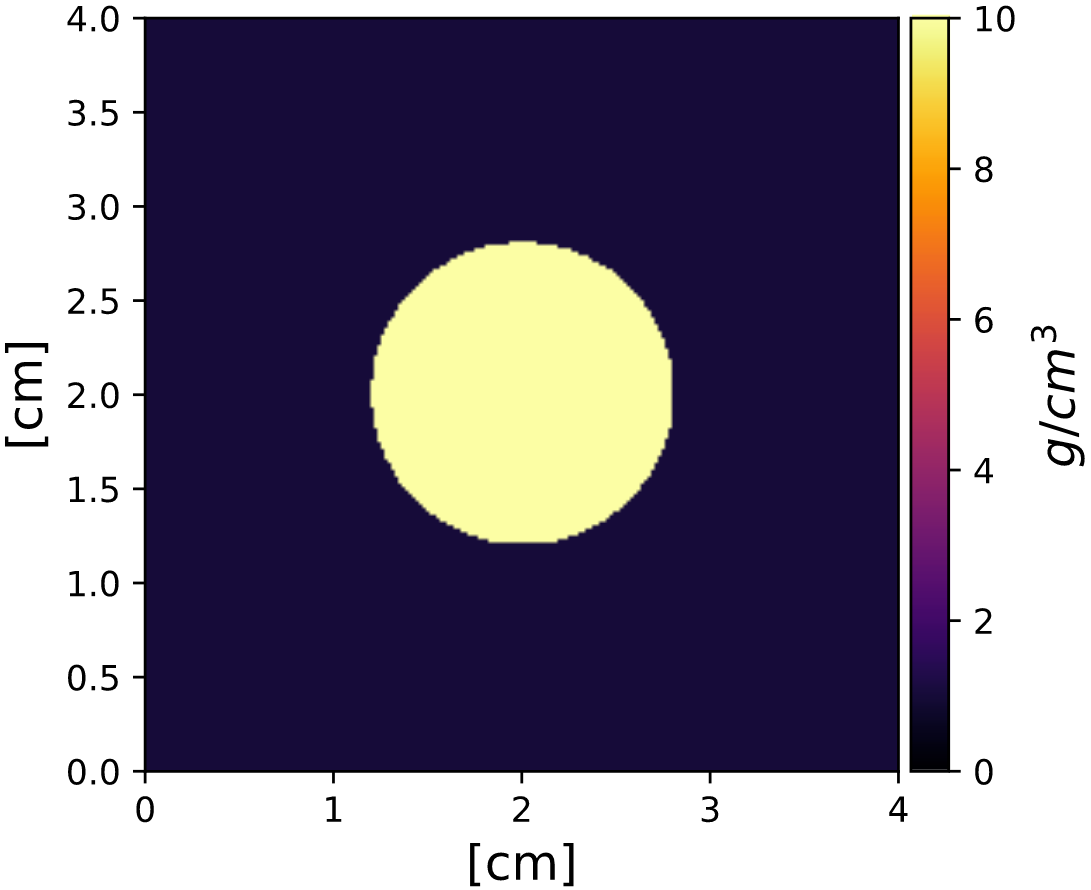
\includegraphics[scale = 0.16]{./Figuras/verificacion_del_codigo/pruebas_2D/head_map/00.png}}
      \subfigure{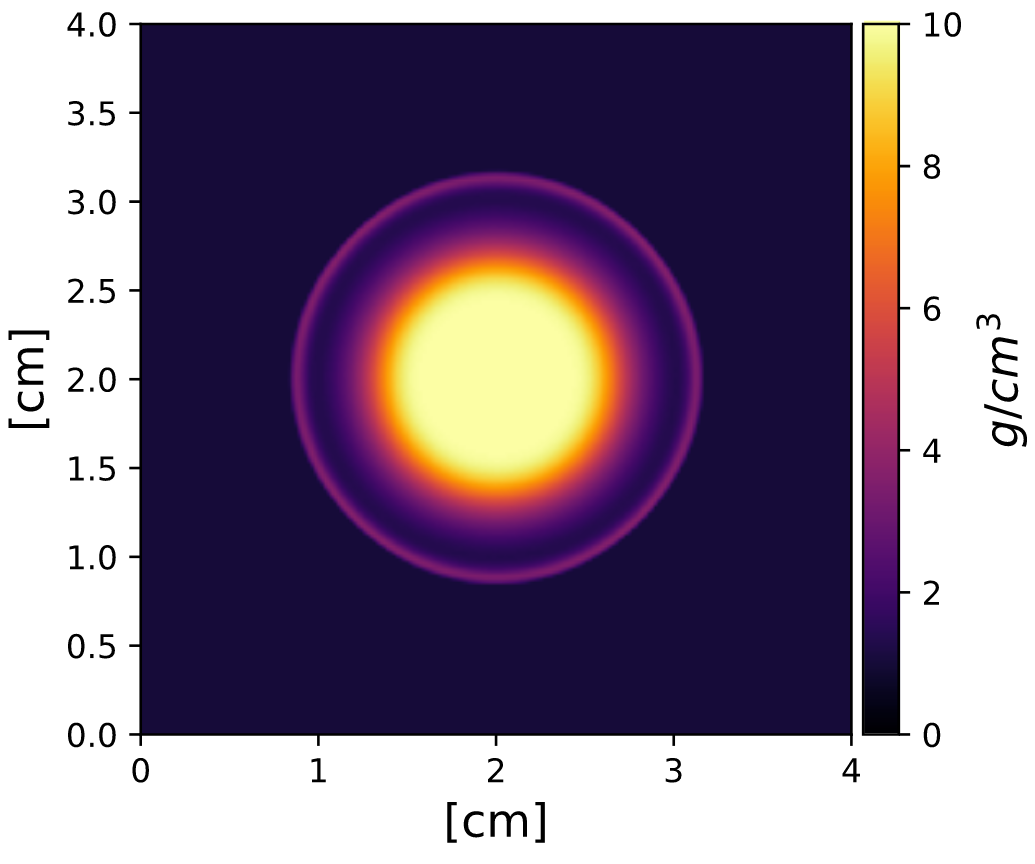
\includegraphics[scale = 0.16]{./Figuras/verificacion_del_codigo/pruebas_2D/head_map/20.png}}
      \subfigure{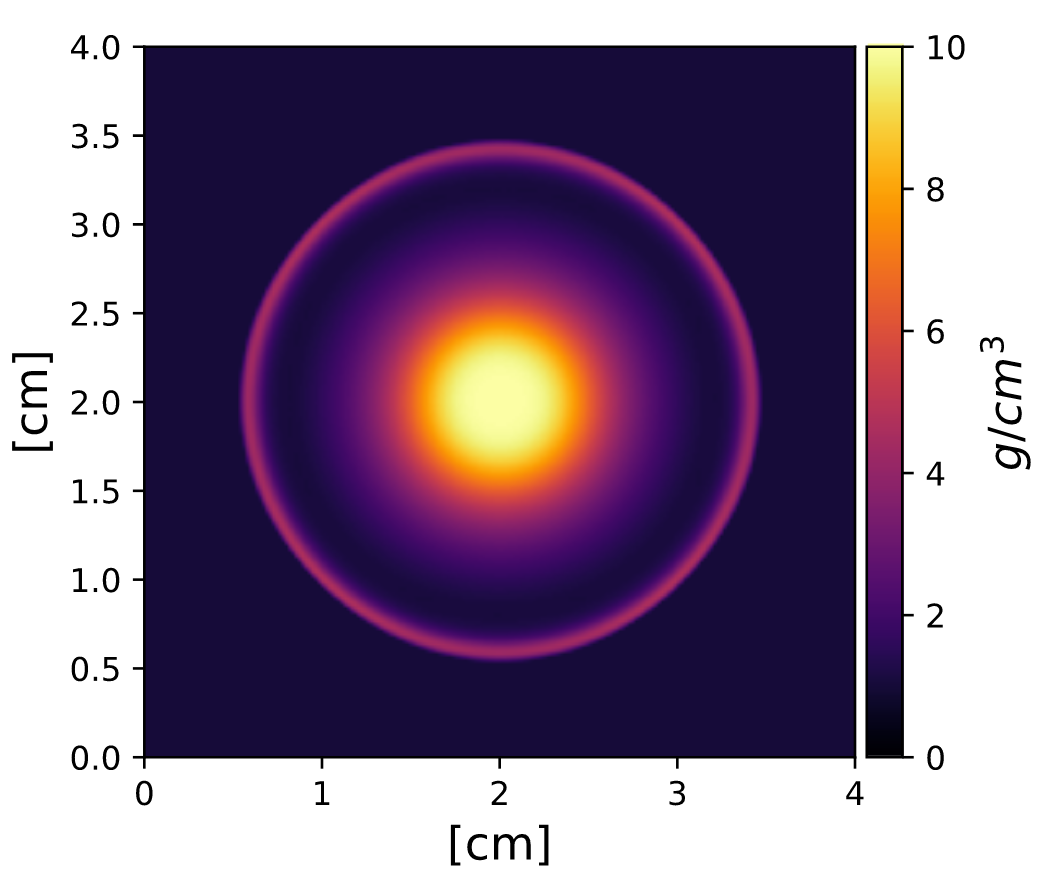
\includegraphics[scale = 0.16]{./Figuras/verificacion_del_codigo/pruebas_2D/head_map/40.png}}
    \caption{Explosión de la onda de choque en 2 dimensiones usando un mapa de calor donde muestra
    la evolución de la densidad. El panel de arriba a la izquierda muestra el tiempo inicial $t=0$ s,
    el de arriba a la derecha  al $t = 0.2$ s y el de abajo al tiempo $t = 0.4$ s. \label{fig:head_map}}
\end{figure}

Antes de compararlo con el perfil unidimensional, primero se comparará entre si mísmo. Es decir, se
compararán los perfiles radiales tomados a 0°, 45°, 90°. 
En la Figura \ref{fig:comparacion_perfil_radial}, el panel de arriba a la izquierda muestra la densidad, 
el de arriba a la derecha la velocidad y el de abajo muestra la presión.

En el panel de arriba a la derecha se muestra una densidad $\rho \approx 10 \, \text{g}/\text{cm}^3$ 
en $x \approx 0.2$
donde comienza a disminuir hasta $\rho \approx 1.5 \, \text{g}/\text{cm}^3$ en $x \approx 0.6$. Después comienza a subir hasta 
$\rho \approx 5 \, \text{g}/\text{cm}^3$ para los perfiles de 90 y 0, mientras que para el de 45 sube hasta 5.5 en el punto
$x \approx 0.7$ cm. Después vuelve a disminuir a $\rho \approx 0 \, \text{g}/\text{cm}^3$ en el punto $x \approx 0.8$ para los 
3 perfiles radiales



Para el perfil de la velocidad (panel arriba a la derecha), 
en $x \approx 0.2$ cm la velocidad empieza a incrementar desde el reposo
$v = 0$ hasta $v \approx 0.7c$ en $x \approx 0.6$ cm, esto aplica para los 3 perfiles de velocidad. Después
va decreciendo hasta $v \approx 0.62c$ en $x \approx 0.75$ cm para los perfiles de 0 y 90, mientras que para 
el perfil de 45 lo hace en $x \approx 0.73$ cm. A partir de este punto la velocidad vuelve a cero.




El el panel de abajo muestra el perfil de la presión. Para el punto $x \approx 0.18$ cm
la presión comienza a disminuir de $p = 13.33 \,  \text{dyn}/ \text{cm}^2$ 
hasta $p \approx 1 \,  \text{dyn}/ \text{cm}^2$ en $x \approx 0.7$ cm para los 
3 perfiles. En $x \approx 0.71 $ cm vuelve a disminuir a $p = 0 \,  \text{dyn}/ \text{cm}^2$ en 
$x \approx 0.74 $ cm para los perfiles de 
0 y 90, mientras que para el perfil de 45 lo hace en $x \approx 0.73 $ cm.

Al comparar las gráficas, se puede ver que los perfiles de 0 y 90, tiene un error del 0\% 
para la densidad, velocidad y presión. Mientras que
al compararse con el de 45 vemos que se tiene un error para la densidad del 0.04 \%,
para la velocidad del 4.8 \% y para la presión del 6.6 \%.

Por lo tanto al no haber una discrepencia grande en los valores de los 3 perfiles radiales podemos ver
que nuestro codigo relativista no cambia a pesar de la dirección que tengan los perfiles radiales de 
densidad, velocidad y presión. Siempre se tiene el mismo perfil en función del radio.

\begin{figure}
  \centering
      \subfigure{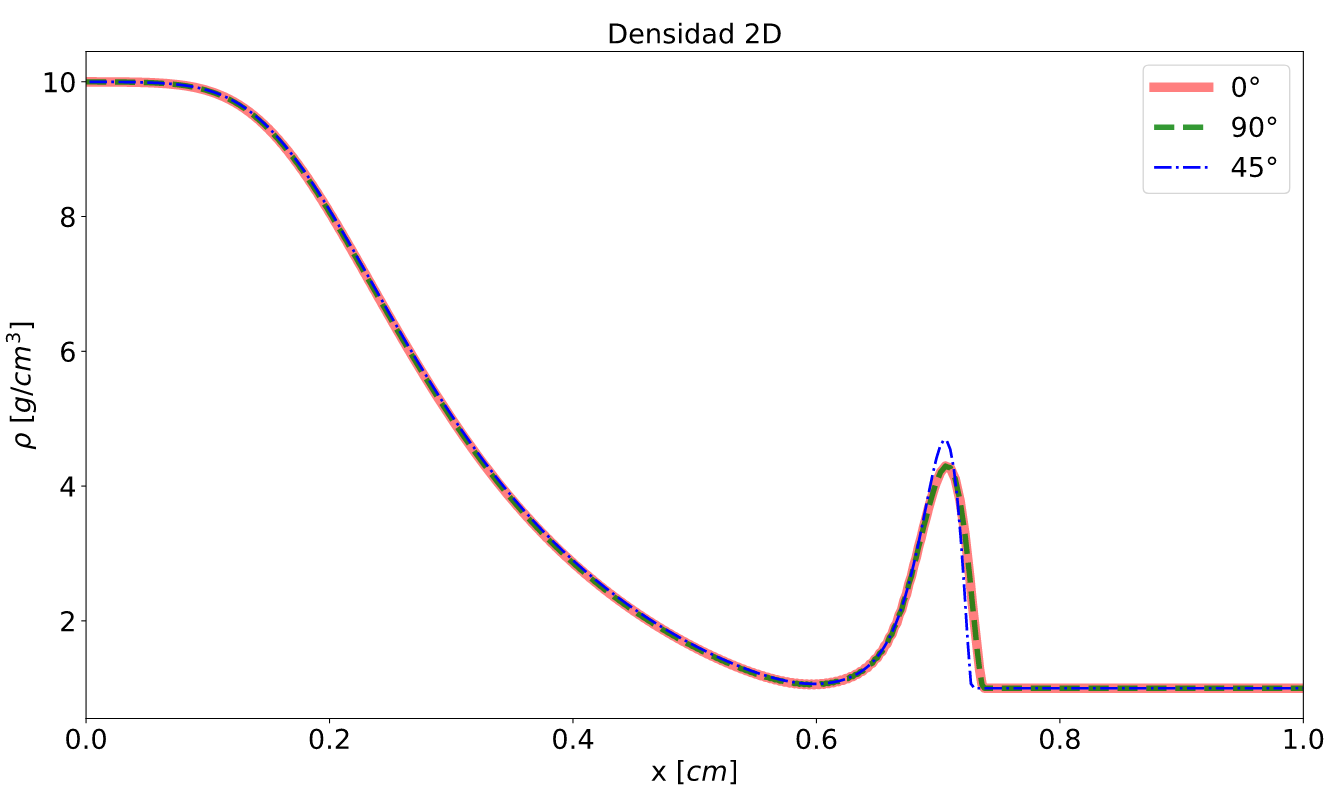
\includegraphics[scale = 0.16]{./Figuras/verificacion_del_codigo/pruebas_2D/combinacion/densidad.png}}
      \subfigure{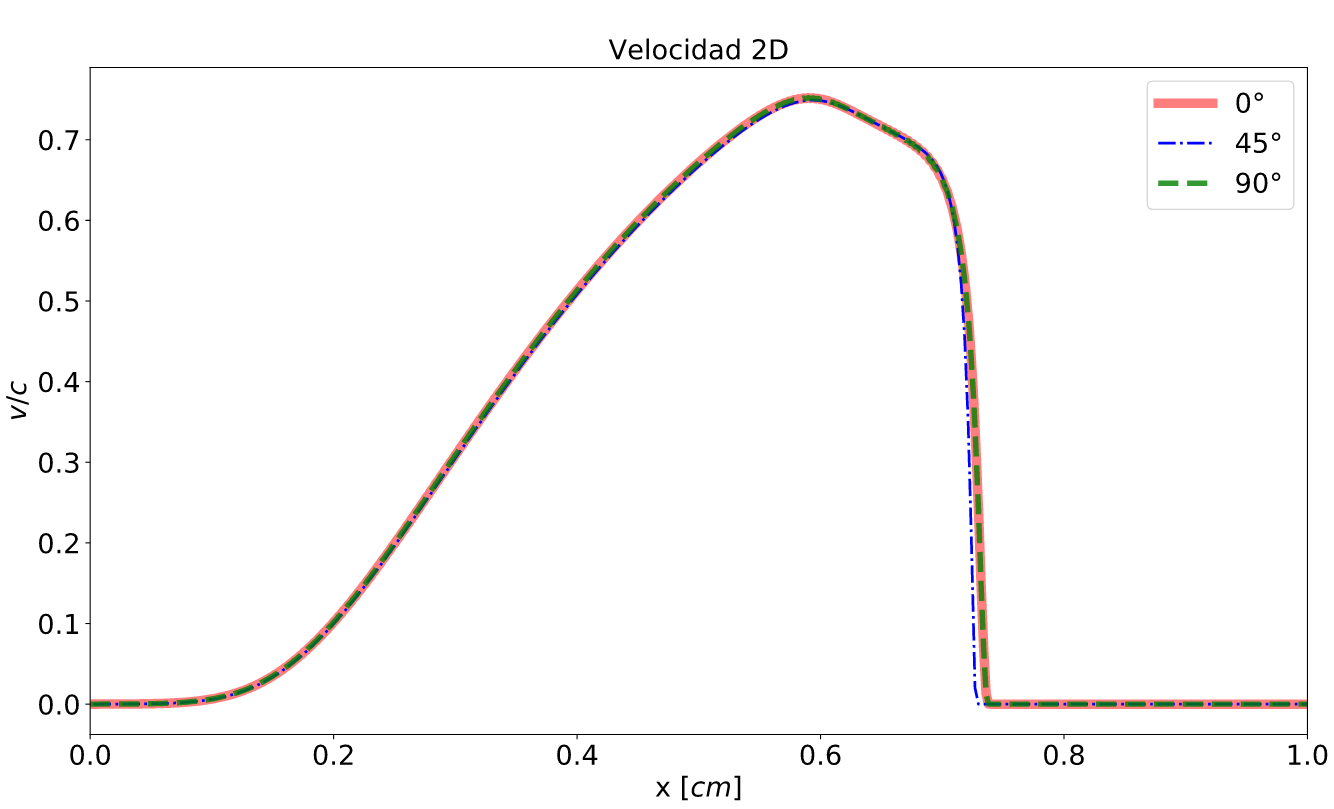
\includegraphics[scale = 0.16]{./Figuras/verificacion_del_codigo/pruebas_2D/combinacion/velocidad.png}}
      \subfigure{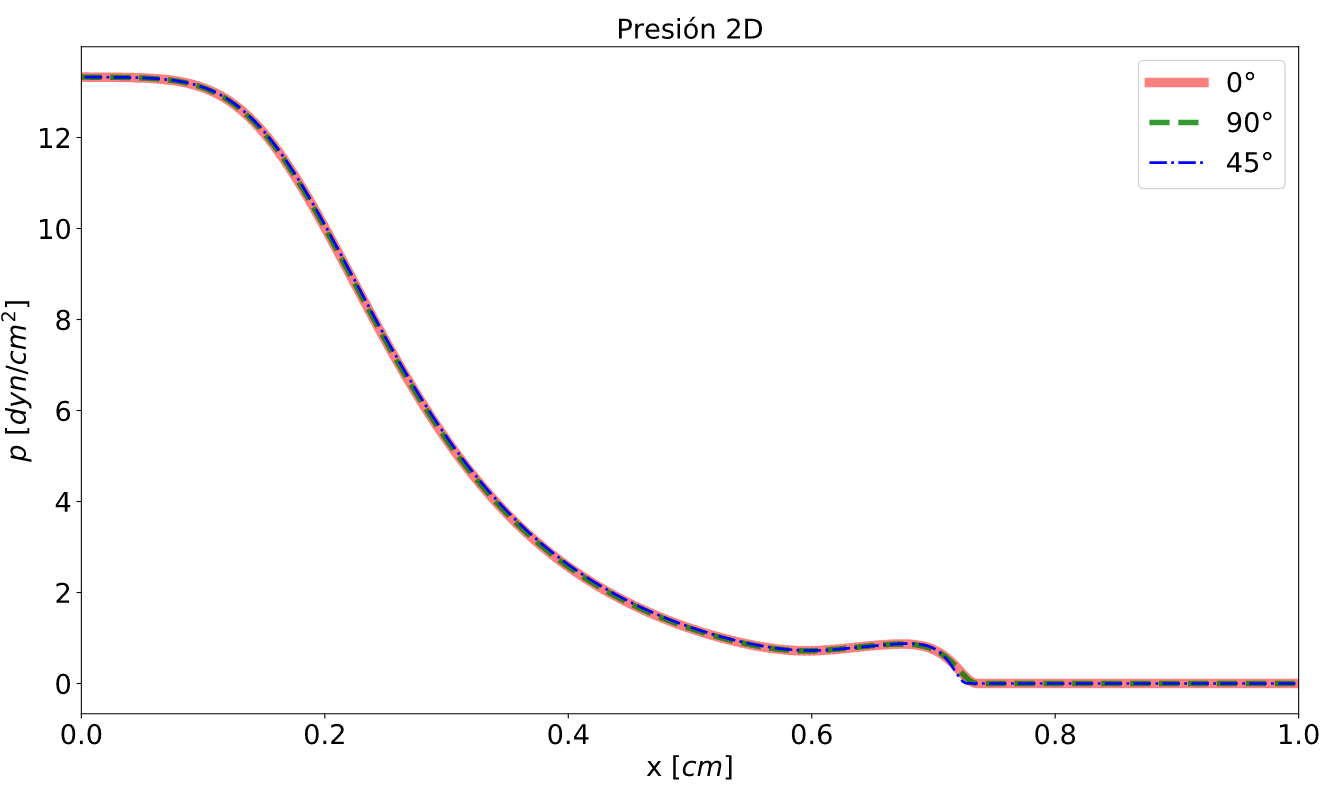
\includegraphics[scale = 0.16]{./Figuras/verificacion_del_codigo/pruebas_2D/combinacion/presion.png}}
    \caption{La figura muestra la comparación que hay entre los distintos perfiles de
    densidad al tiempo $t = 0.4$ s. El panel de arriba a la izquierda muestra el perfil a 0° (linea roja
    sólida), el de arriba a la derecha muestra a 90° (linea verde punteada) y el panel de abajo 
    (linea azul de raya y punto) muestra a 45°}
    \label{fig:comparacion_perfil_radial}
\end{figure}


En la Figura \ref{fig:comparacion_perfil_mean} muestra la comparación entre la prueba unidimensional
y la prueba bidimensional, que es la media de los 3 perfiles radiales que se tomaron.
El panel de arriba a la izquierda muestra la densidad, el de arriba a la derecha, la velocidad y 
el de abajo la presión.
La densidad y presión, para ambas pruebas, mantienen sus valores de 
$\rho = 10 \,  \text{g}/ \text{cm}^3$ y $p = 13.33 \,  \text{dyn}/ \text{cm}^2 $ 
luego, bajan sus valores en $x \approx 0.25$ cm
mientras que la velocidad , la cual es nula,
asciende. En el punto $x \approx 0.68$ cm la presión alcanza 
$p \approx 2.0\,  \text{dyn}/ \text{cm}^2 $ y la densidad
$\rho \approx 2.0 \,  \text{g}/ \text{cm}^3$, mientras que la velocidad sube a $v \approx 0.75c$
en una dimensión. En 2 dimensiones la densidad baja hasta  $\rho \approx 1.0 \,  \text{g}/ \text{cm}^3$ y
la presión $p \approx 1.8\,  \text{dyn}/ \text{cm}^2 $ mientras que la velocidad en $x \approx 0.68$ cm
sube a $v \approx 0.8c$ y baja a $v \approx 0.7c$ en $x \approx 0.68$ cm


\begin{figure}
  \centering
      \subfigure{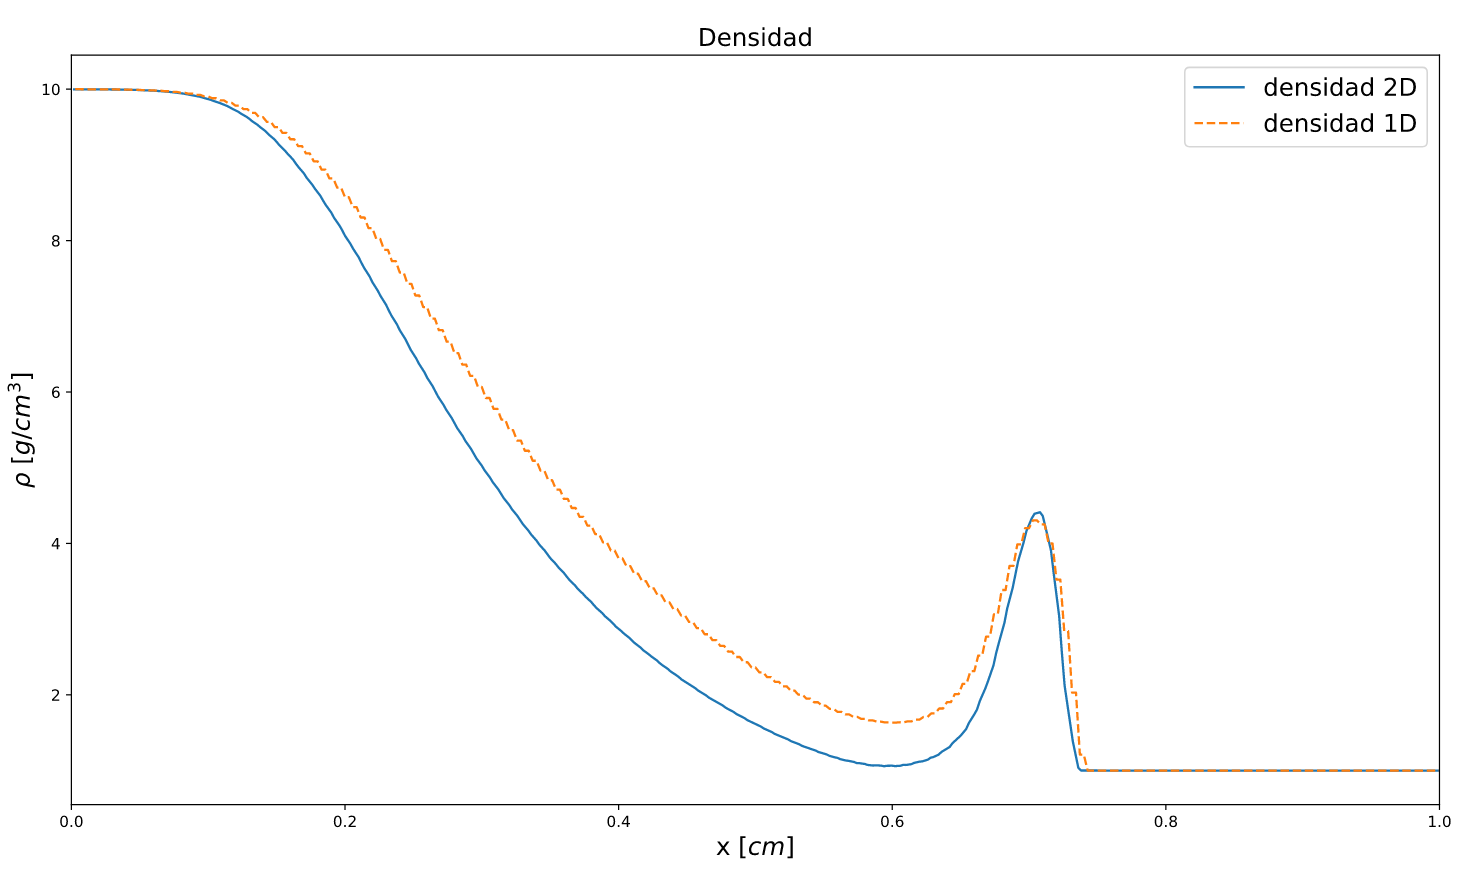
\includegraphics[scale = 0.16]{./Figuras/verificacion_del_codigo/pruebas_2D/mean/densidad.png}}
      \subfigure{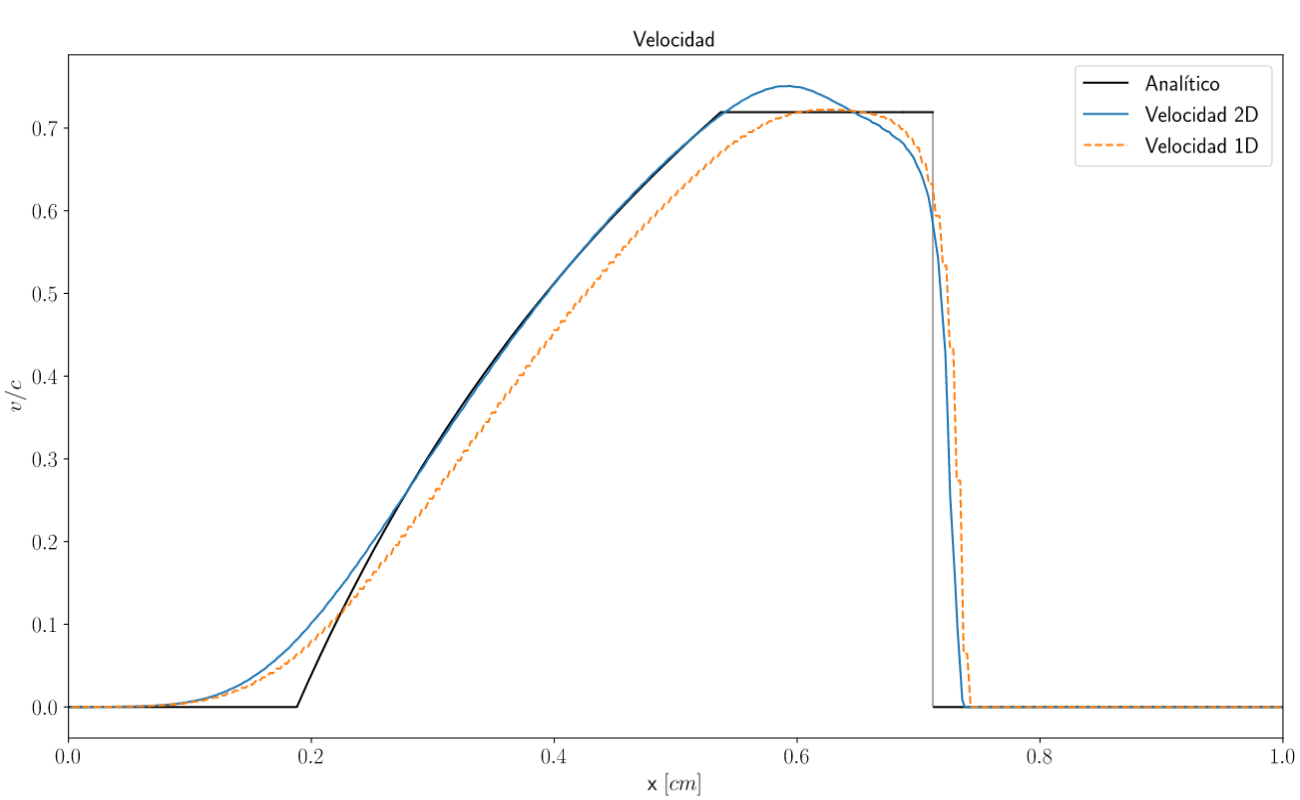
\includegraphics[scale = 0.16]{./Figuras/verificacion_del_codigo/pruebas_2D/mean/velocidad.png}}
      \subfigure{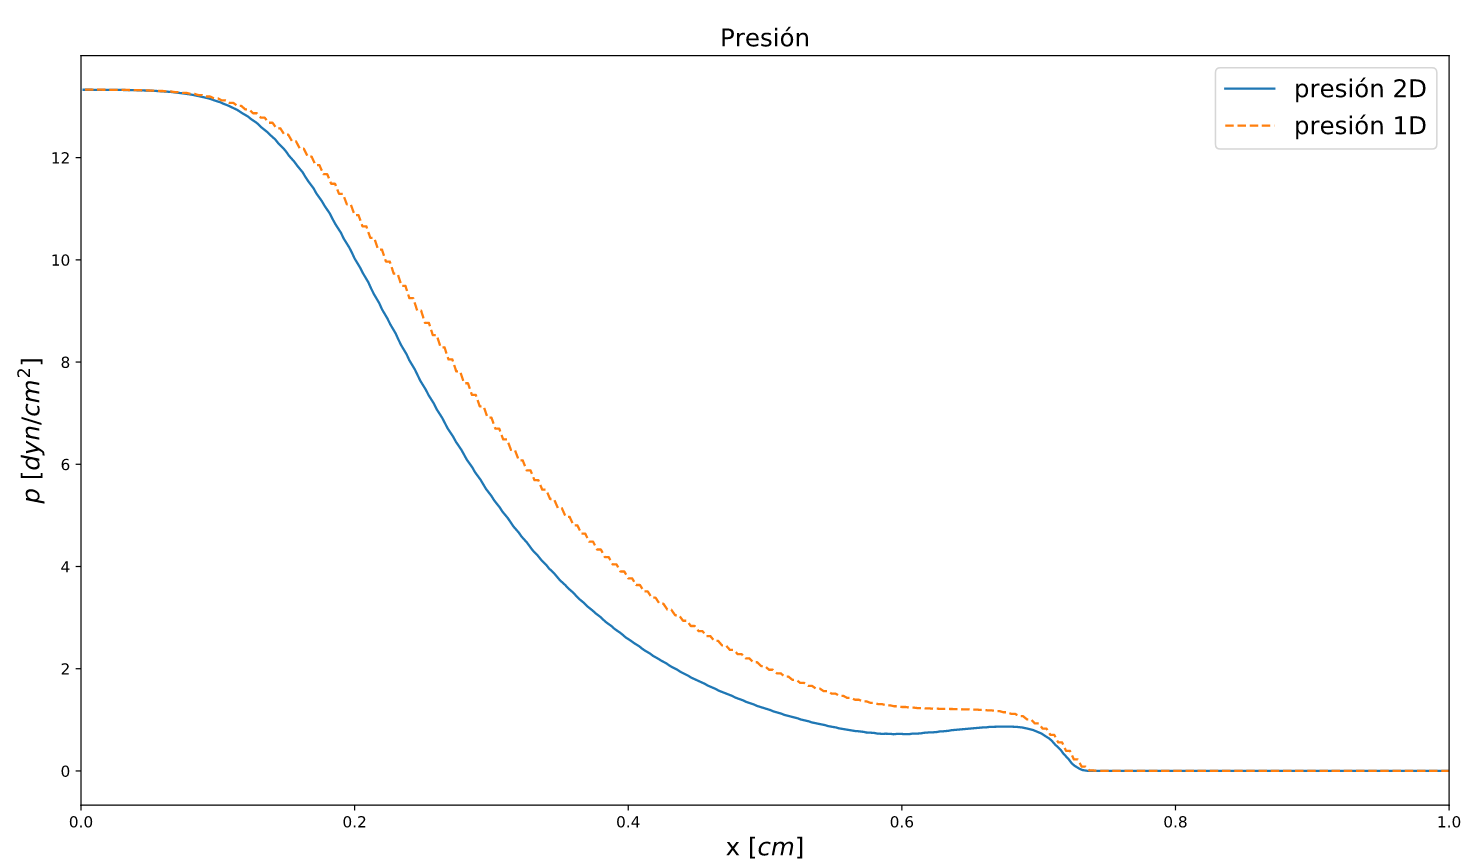
\includegraphics[scale = 0.16]{./Figuras/verificacion_del_codigo/pruebas_2D/mean/presion.png}}
    \caption{Comparación entre la media de los 3 perfiles radiales (linea sólida azul), la 
    la prueba unidimensional (linea de puntos rojos) y la analítica (linea negra sólida)
    .}\label{fig:comparacion_perfil_mean}
\end{figure}


La densidad en 1D como en 2D vuelve a subir
en $x \approx 0.69$ cm y llega a $\rho \approx 5 \,  \text{g}/ \text{cm}^3$ y 
se mantiene así hasta el punto $x \approx 0.7$ cm 
donde la densidad, así como la velocidad y presión descienden sus valores a nulos.

La mayor diferencia que hay entre la 1D y 2D para la densidad es del 70 \%, mientras que para la 
velocidad es del 238 \% y la de la presión es del 79 \%.

Al comparar los perfiles bidimensionales con el analítico, para la densidad se tiene un error del
13 \%, para la velocidad del 12 \% y para la presión del 16 \%. Luego al comparar el unidimensional
con el analítico, la densidad es del 3 \%, la velocidad del 7\% y la presión del 4 \%.

Al no haber tanta diferencia del resultado de la media de los perfiles radiales bidimensionales con 
los perfiles unidimensionales y con el analítico puedo concluir que mi código relativista es válido
para 2 dimensiones.



% % ========================================= caso_10 ========================================================================

% \begin{figure}
%   \centering
%     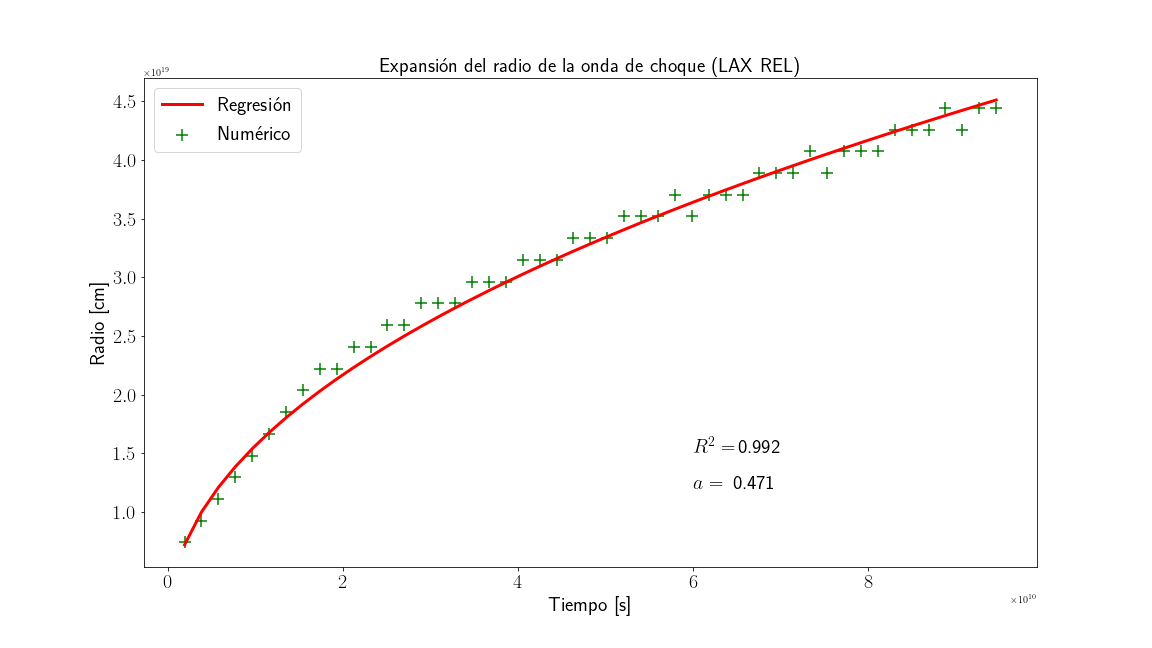
\includegraphics[width=0.8\textwidth]{./Figuras/verificacion/casos/caso_10/Expansion}
%   \caption{Velocidad del radio de expansión de una onda de choque conforme avanza el tiempo. El eje del tiempo tiene un factor de $10^{10}$ mientras que el del radio
%   un factor de $10^19$. La ecuación con la que se expande la onda es $ Radio = 522773497555577.4 t^{0.4409}$ con un coeficiente de relación $R^2=0.9916$
%   } \label{fig_velocidad_vs_radio_computacionalmente}
% \end{figure}



% \begin{figure}
%   \centering
%   \subfigure[$t = 0 $ s]{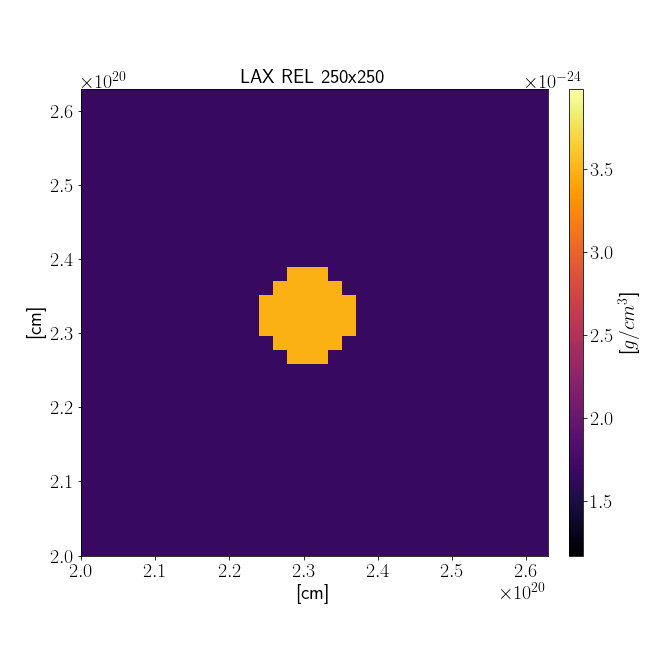
\includegraphics[scale = 0.36]{./Figuras/verificacion/casos/caso_10/LAX_REL_screenshot_0}}
%   \subfigure[$t = 1.89\,\times 10^{10}$ s]{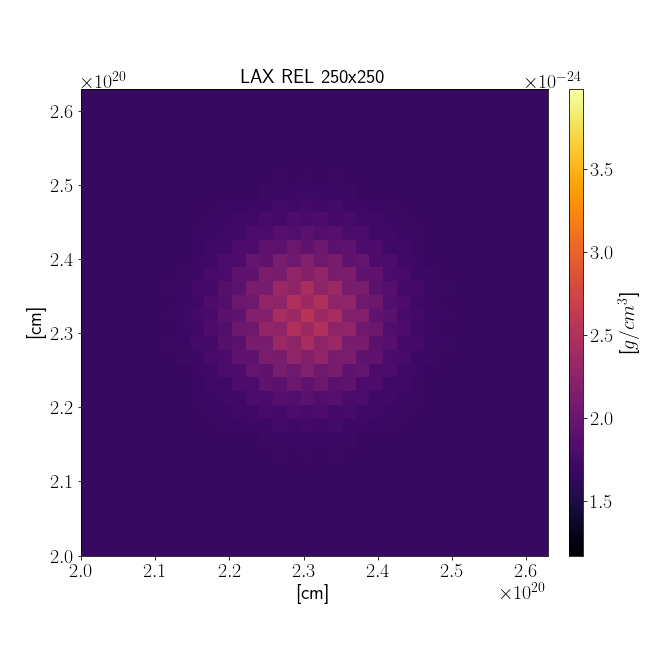
\includegraphics[scale = 0.36]{./Figuras/verificacion/casos/caso_10/LAX_REL_screenshot_20}}
%   \subfigure[$t = 3.784 \,\times 10^{10}$ s]{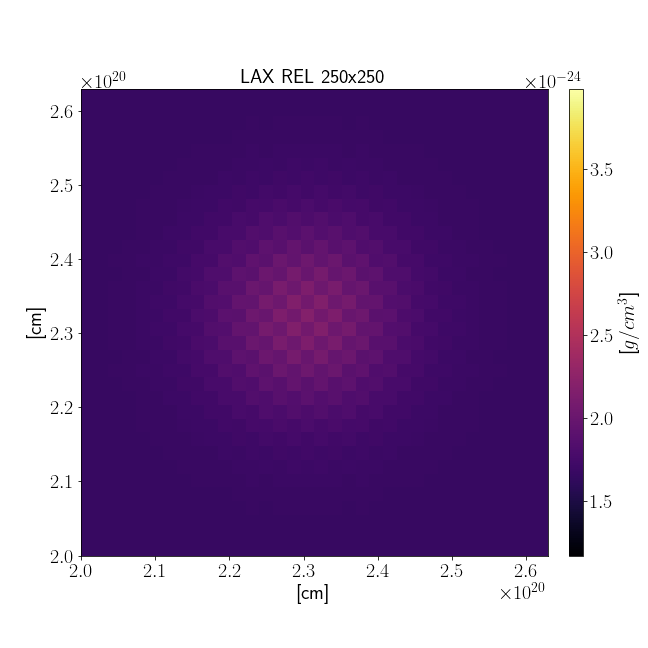
\includegraphics[scale = 0.36]{./Figuras/verificacion/casos/caso_10/LAX_REL_screenshot_40}}
%   \caption{Evolución de la onda de choque de la Figura \ref{fig_velocidad_vs_radio_computacionalmente}}
% \end{figure}
%   % ========================================= caso_10 ========================================================================


% % ========================================= caso_11 ========================================================================

% \begin{figure}
%   \centering
%     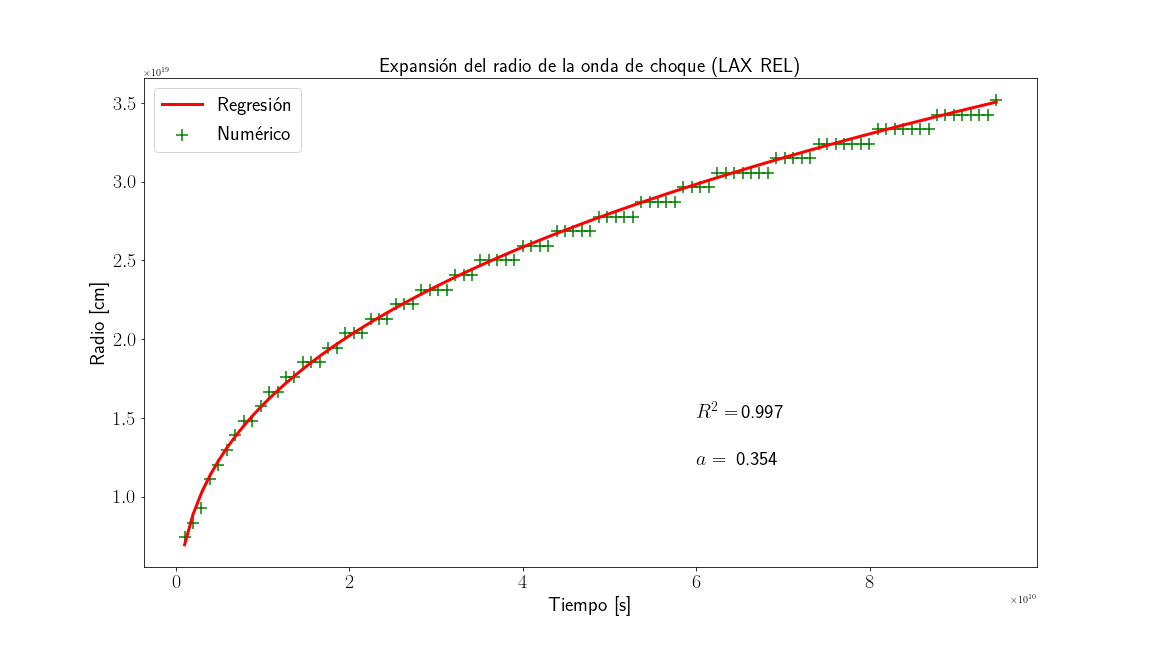
\includegraphics[width=0.8\textwidth]{./Figuras/verificacion/casos/caso_11/Expansion}
%   \caption{Velocidad del radio de expansión de una onda de choque conforme avanza el tiempo. El eje del tiempo tiene un factor de $10^{10}$ mientras que el del radio
%   un factor de $10^19$. La ecuación con la que se expande la onda es $ Radio = 522773497555577.4 t^{0.4409}$ con un coeficiente de relación $R^2=0.9916$
%   } \label{fig_velocidad_vs_radio_computacionalmente}
% \end{figure}



% \begin{figure}
%   \centering
%   \subfigure[$t = 0 $ s]{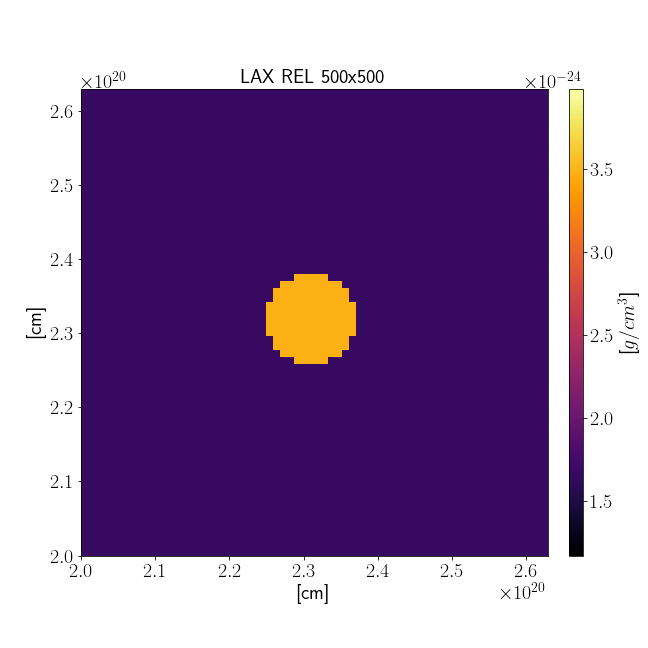
\includegraphics[scale = 0.36]{./Figuras/verificacion/casos/caso_11/LAX_REL_screenshot_0}}
%   \subfigure[$t = 1.89\,\times 10^{10}$ s]{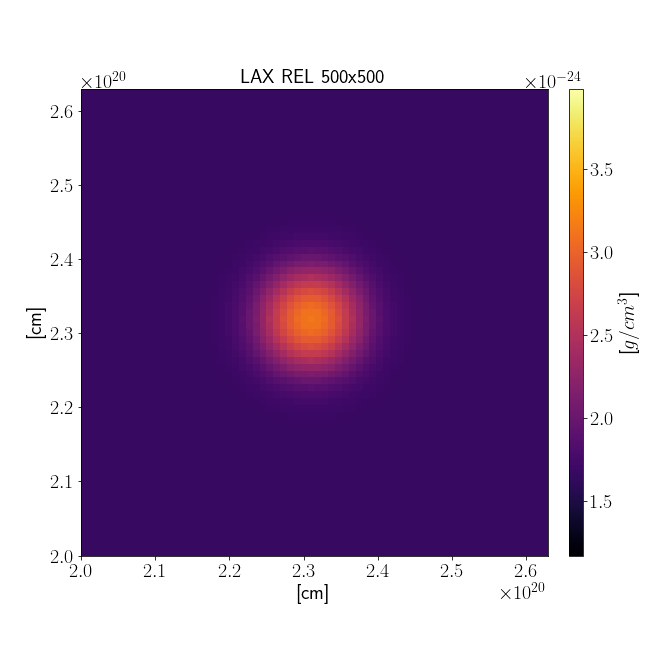
\includegraphics[scale = 0.36]{./Figuras/verificacion/casos/caso_11/LAX_REL_screenshot_20}}
%   \subfigure[$t = 3.784 \,\times 10^{10}$ s]{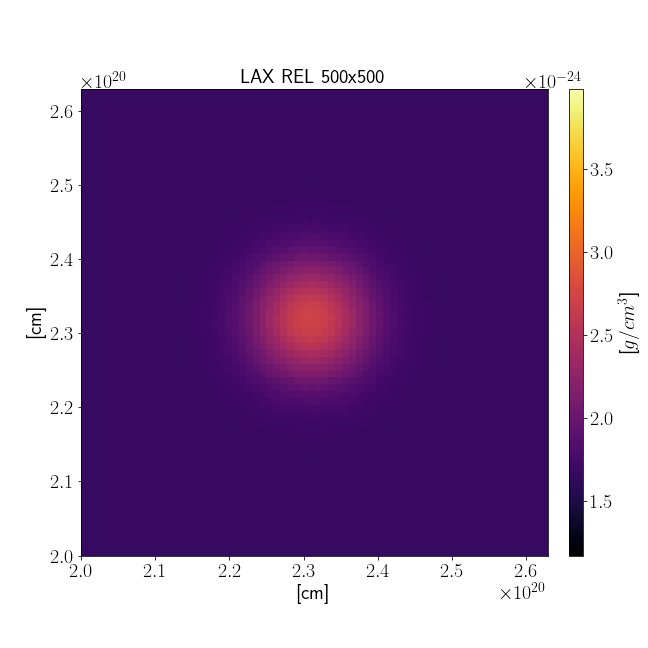
\includegraphics[scale = 0.36]{./Figuras/verificacion/casos/caso_11/LAX_REL_screenshot_40}}
%   \caption{Evolución de la onda de choque de la Figura \ref{fig_velocidad_vs_radio_computacionalmente}}
% \end{figure}
%   % ========================================= caso_11 ========================================================================


% % ========================================= caso_12 ========================================================================

% \begin{figure}
%   \centering
%     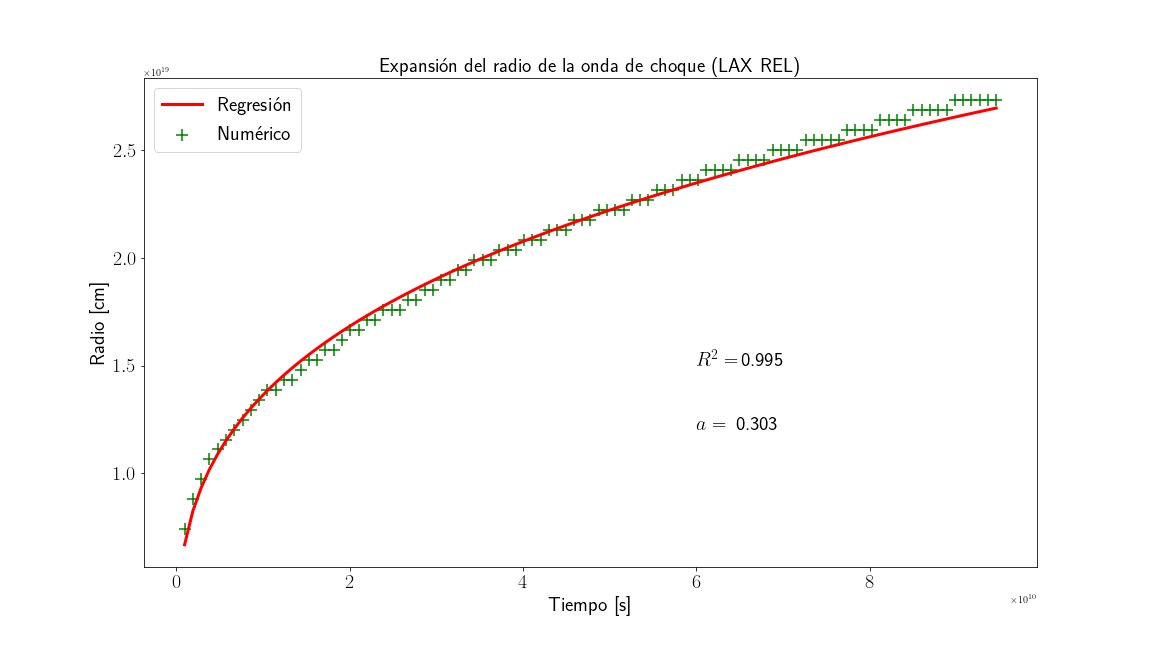
\includegraphics[width=0.8\textwidth]{./Figuras/verificacion/casos/caso_12/Expansion}
%   \caption{Velocidad del radio de expansión de una onda de choque conforme avanza el tiempo. El eje del tiempo tiene un factor de $10^{10}$ mientras que el del radio
%   un factor de $10^19$. La ecuación con la que se expande la onda es $ Radio = 522773497555577.4 t^{0.4409}$ con un coeficiente de relación $R^2=0.9916$
%   } \label{fig_velocidad_vs_radio_computacionalmente}
% \end{figure}



% \begin{figure}
%   \centering
%   \subfigure[$t = 0 $ s]{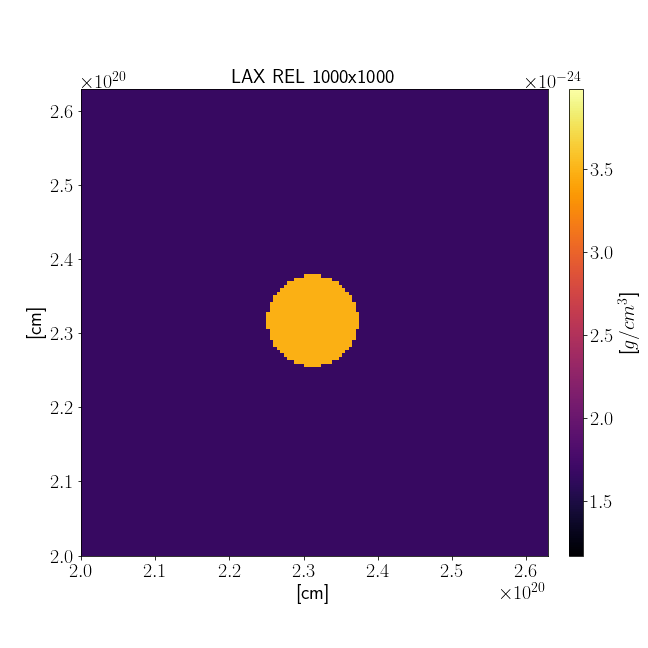
\includegraphics[scale = 0.36]{./Figuras/verificacion/casos/caso_12/LAX_REL_screenshot_0}}
%   \subfigure[$t = 1.89\,\times 10^{10}$ s]{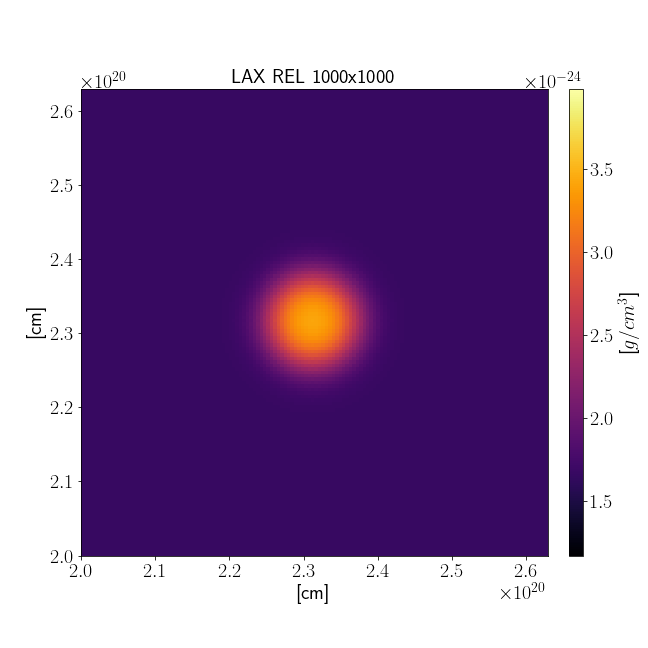
\includegraphics[scale = 0.36]{./Figuras/verificacion/casos/caso_12/LAX_REL_screenshot_20}}
%   \subfigure[$t = 3.784 \,\times 10^{10}$ s]{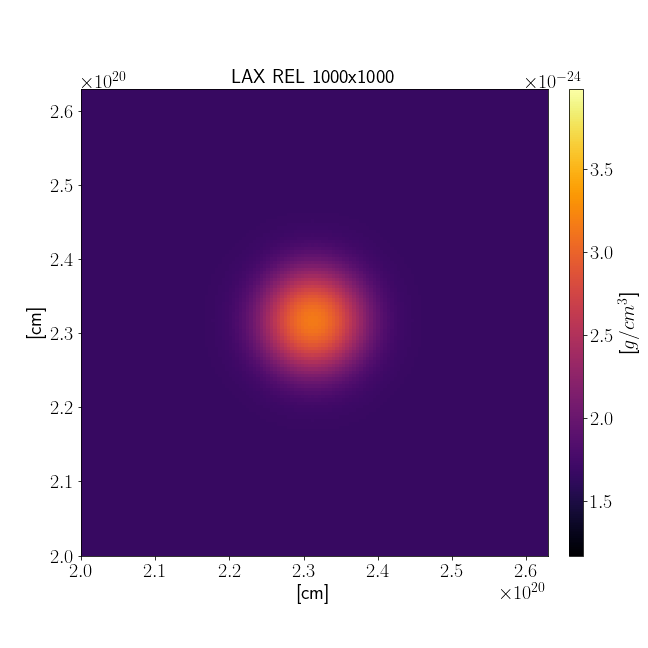
\includegraphics[scale = 0.36]{./Figuras/verificacion/casos/caso_12/LAX_REL_screenshot_40}}
%   \caption{Evolución de la onda de choque de la Figura \ref{fig_velocidad_vs_radio_computacionalmente}}
% \end{figure}
%   % ========================================= caso_12 ========================================================================





% \section{Onda de choque} \label{sec:onda de choque}%Shock Wave and High Pressure Phenomena) Isabelle Sochet (eds.
% La onda de choque se produce por la liberación rápida de energía comprimida dentro de un volumen de radio $R$. Esta explosión divide a nuestro dominio en 2 
% zonas distintas como se muestra en la Figura \ref{fig:onda_choque_example}. La zona I, estará determinado por la densidad, presión, y velocidades del medio 
% ambiente ($\rho_m, \, P_m\, v_{x_m}, \, v_{y_m}$, respectivamente). La zona II (i.e. dentro de la onda de choque), se produce al depositar una densidad de 
% energía $E_{in}$ dentro de una región definida por un radio interno ($R_{in}$) en reposo. Para ver más detalles véase el cuadro \ref{fig:onda_choque_example}.

% \begin{table}[htbp]
% \begin{center}
% \begin{tabular}{|c|c|c|}
% \hline 
% \textbf{Parámetro} & \textbf{Descripción} & \textbf{valor} \\ 
% \hline 
% $R_{in}$ & Radio interno de la onda expansiva & 0.2 [cm] \\ 
% \hline 
% $\rho_{in}$ &  Densidad interna de la onda expansiva & 5.0 [$\mathrm{g} \cdot \mathrm{cm}^{-3}$] \\ 
% \hline 
% $\rho_{out}$ &  Densidad del medio  & 1.0 [$\mathrm{g} \cdot \mathrm{cm}^{-3}$] \\
% \hline 
% $P_{int}$ & Presión interna de la onda expansiva & 10.0 [$ \mathrm{erg}\cdot \mathrm{cm}^{-2}$]\\ 
% \hline 
% $P_{out}$ &  Presión del medio  & 0.1 [$\mathrm{erg}\cdot \mathrm{cm}^{-2}$] \\ 
% \hline 
% $v_{x_{int}}$ & Velocidad interna en el eje x de la onda expansiva & 0.0 [$\mathrm{cm}\cdot \mathrm{s}^{-1}$]\\ 
% \hline 
% $v_{y_{int}}$ & Velocidad interna en el eje y de la onda expansiva & 0.0 [$\mathrm{cm}\cdot \mathrm{s}^{-1}$]\\ 
% \hline 
% $v_{x_{out}}$ & Velocidad en el eje x del medio & 0.0 [$\mathrm{cm}\cdot \mathrm{s}^{-1}$] \\
% \hline 
% $v_{y_{out}}$ & Velocidad en el eje y del medio & 0.0 [$\mathrm{cm}\cdot \mathrm{s}^{-1}$]\\ 
% \hline 
% Co & Número de Courant & 0.7 \\ 
% \hline 
% \end{tabular}
% \caption{\label{Tabla_parametros}Parámetros que se utilizarán en las siguientes pruebas que se van a realizar para la onda de choque, estos valores son para fluidos newtonianos.}
% \end{center}
% \end{table}

% La densidad de energía $E_{in}$ de la onda de choque está determinada por $\rho_{in}$, $P_{in}$, y $v_{x_{in}}$ y $v_{y_{in}}$ ya que es la suma de la energía cinética más la energía térmica
% $E_{in} = {\frac{1}{2}} \rho_{in} v_{in}^2 + {\frac{P_{in}}{\Gamma -1 }}$).
% Dado que la zona II está en reposo $v_{x_{in}}=0$ y $v_{y_{in}}=0$, se tiene:
% $E_{in} = {\frac{P_{in}}{\Gamma -1 }}$).
% Cabe señalar que los valores de la densidad y presión del medio ambiente tendrán valores mas bajos que sus respectivos de la onda de choque. 

% \begin{figure}
% \centering
% \includegraphics[width=0.6\textwidth]{./Figuras/Pruebas/Prueba_onda_choque/prueba_example}
% \caption{\label{fig:onda_choque_example}La zona I (medio ambiente), se caracterizará por tener valores de densidad, presión y velocidades ($\rho_m, \, P_m \, v_{x_m}, \, v_{y_m}$, respectivamente) mostrados en el cuadro \ref{Tabla_parametros}. La zona II (onda de choque) se produce al depositar una energía ($E_{in}$) y una presión ($P_{in}$) dentro de un círculo (con $R_{in}$).}
% \end{figure}

% La onda de choque se dejó evolucionar con el paso del tiempo, y se analizó la interacción que hay entre las zonas I y II. En específico, se siguió la evolución de una onda de choque con una velocidad de expansión muy por debajo de la velocidad de la luz (caso newtoniano), y además la evolución de una onda de choque cuya velocidad de expansión estaba cercana a la velocidad de la luz (caso relativista). Cabe señalar que en ambos casos se siguieron los cambios que se produjeron utilizando los método numéricos de Lax y el de HLL (véase la Sección \ref{sec:Diferencias_finitas} para mayor información). La condición a la frontera utilizada en todos los bordes fue la de \emph{outflow}\footnote{Para ver más detalles acerca de esta frontera y/o de otro tipo de fronteras veáse el apéndice \ref{aped.B}}. 


% %tiempo = 0.5 s
% %lapso = tiempo/20



% \subsection{Caso newtoniano} \label{subs:caso_newtoniano}
% %\subsubsection{Lax} \label{subsec: Prueba Lax}
% %Como primeras pruebas se realiza: explicas la 3.2, y además se llevó a cabó (explicas la Figura 3.5).

% %Las dos primeras pruebas: 

% %1. Newtoniano + Lax + onda choque centrada 2. Newtoniano + Lax + onda choque borde

% Las siguientes pruebas fueron usando el método de Lax, como este es un caso newtoniano, La constante de relacion específica es $\Gamma = 5/3$. La descripción del fenómeno es de una onda expansiva sobre un medio constante (ver Figura \ref{fig:onda_choque_example}) 
% con una densidad de energía de $e = 0.15 \, \mathrm{erg} \cdot \mathrm{cm}^{-3}$, densidad $\rho = 1 \, \mathrm{g} \cdot \mathrm{cm}^{-3}$ , velocidades $v = 0 \, \mathrm{cm} \cdot \mathrm{s}^{-1}$ y una presión $P=0.1 \, \mathrm{erg} \cdot \mathrm{cm}^{-3} $. La simulación es sobre un dominio de 0 a 1 cm sobre el eje \emph{x} y de 0 a 1 cm sobre el eje \emph{y}, con una resolución de 500x500 píxeles\footnote{Los píxeles de nuestra malla miden $l_x\cdot 500^{-1} = l_y\cdot 500^{-1}  = 1 \, \mathrm{cm} \cdot 500^{-1} = 0.005 \, \mathrm{cm}$} al tiempo $t=0 \, \mathrm{s}$  y en la onda interna. La densidad de la onda es $\rho=5 \, \mathrm{g} \cdot \mathrm{cm}^{-3}$, la velocidad interna será la misma que la del ambiente, la presión interna $P=10 \, \mathrm{erg} \cdot \mathrm{cm}^{-3} $ 
% y una densidad de energía interna $e = 3.75 \, \mathrm{erg} \cdot \mathrm{cm}^{-3}$. La onda de choque esta centrada en el punto $(x,y) = (0.5, 0.5) \, \mathrm{cm}$, y se corrió en el intervalo de tiempo $t \in \left[ 0 , 0.2 \right]$ s.
% %%===================IMAGE_LAX_CENTRADO_T=0===============================
% %\begin{figure}[H]
% %\centering
% %\includegraphics[width=0.5\textwidth]{./Figuras/Pruebas/Prueba_onda_choque/onda_choque1_t_0}
% %\caption{Condición inicial ($t = 0$) de una onda de choque (con $\rho_{in}=5.0, \, v_{x_{in}}=v_{y_{in}}=0.0, \, P_{in}=10.0$ y $E_{in}=3.75$), de radio interno $R_{in} = 0.2$ cm. que se va a expandir sobre un medio (con $\rho_{out}=1.0$  y $ P_{out}=0.1$) estático. Véase el Cuadro \ref{Tabla_parametros} para más detalles.} \label{fig:onda_choque1_t_0}
% %\end{figure}
% %%===================IMAGE_LAX_CENTRADO_T=0===============================
% \subsubsection{Lax}
% La evolución para la onda de choque newtoniano muestra una expansión simétrica como se ve en la Figura \ref{fig:Lax-newtoniano_sedov-3-5}. La velocidad de la onda en los primeros instantes es rápida, pero se vuelve constante y mantiene una velocidad $v_{lax} = 1.50 \, \mathrm{cm} \cdot \mathrm{s}^{-1}$ (ver Figura \ref{fig:expansion_radial_newtoniano}).


% % El radio de la onda al tiempo inicial fue de $r=0.2$ cm. A $t=0.05$ s la onda se expandió a un radio de $r=0.3$~cm mientras que para el tiempo $t=0.10$ s se expandió a un radio de $r=0.38$~cm. Debido a lo anterior, la velocidad de expansión de la onda fue de $v = 2.0 \, \mathrm{cm} \cdot \mathrm{s}^{-1}$ y $v = 1.8 \, \mathrm{cm} \cdot \mathrm{s}^{-1}$, respectivamente.% FALTA MENCIONAR A FORWARD SHOCK Y LA REVERSE SHOCK.. y por ende el HUECO (ver Figura \ref{fig:Lax-newtoniano-prueba1}). ADMÄS FALTA MENCIONAR QUE LA PARTE CENTRAL SE DIFUMINA... LO CUAL ES ESPERABLE DEBIDO A LA VISCOSIDAD NUMERICA.


% %===================IMAGE_LAX_CENTRADO_EVOLUCION===============================
% \begin{figure}
% \centering
% \subfigure[$t = 0.05$ s]{\includegraphics[scale = 0.55]{./Figuras/Pruebas/Prueba_onda_choque/Lax/Lax-sedov3}}
% \subfigure[$t = 0.1$ s]{\includegraphics[scale = 0.55]{./Figuras/Pruebas/Prueba_onda_choque/Lax/Lax-sedov5}}
% \caption{\label{fig:Lax-newtoniano_sedov-3-5}Evolución de la onda de choque mostrada en la Figura \ref{fig:onda_choque_example} usando el método de Lax newtoniano. En el panel a) se muestra la onda de choque a t=0.05s, mientras que en el panel b) se muestra para t=0.10 s. En la Figura \ref{fig:Lax-newtoniano-prueba1-analisis} se analizará más a fondo las partes que se forman al desarrollarse dicha onda.}
% \end{figure}
% %===================IMAGE_LAX_CENTRADO_EVOLUCION===============================


% Cuando la onda se empieza a expandir por el medio constante, aparecen 5 áreas distintas que interactuan entre nuestro medio ambiente y la onda. El área 1 (ver Figura \ref{fig:Lax-newtoniano-prueba1-analisis}) es el material al cual la onda no ha tocado y que se cataloga como la del medio ambiente. En el área 2, se muestra una onda que va chocando con el material del medio ambiente, a esta onda la llamaremos \emph{forward shock}\footnote{La palabra \emph{forward shock} viene del inglés y la podemos interpretar como choque hacia adelante. }. El área 3 presenta el material chocado con el mismo centro de la onda, esta se caracteriza por ir en reversa y llamaremos \emph{reverse shock}\footnote{La palabra \emph{reverse shock} viene del inglés y la podemos traducir como choque hacia atras}. El material contra el cual aún no ha chocado la onda es el área 5. La separación que hay entre estas 2 ondas vas creando un vacio que se ve difuminado, esto debido a la viscosidad que presenta nuestro resolvedor de Riemann.


% %===================IMAGE_LAX_CENTRADO_EVOLUCION_ANALISIS===============================
% \begin{figure}
% \centering
% \subfigure[$t = 0.05$ s]{\includegraphics[scale = 0.42]{./Figuras/Pruebas/Prueba_onda_choque/Lax/Lax-sedov3-analisis}}
% \subfigure[$t = 0.1$ s]{\includegraphics[scale = 0.425]{./Figuras/Pruebas/Prueba_onda_choque/Lax/Lax-sedov5-analisis}}
% \caption{\label{fig:Lax-newtoniano-prueba1-analisis}En la evolución de la onda usando el método de Lax,  se encuentran 5 áreas distintas. El área 1 la identificaremos como el material que no ha sido chocado todavía por nuestra onda. El área 2 será el material que es chocado por nuestra onda, esta onda que se llama \emph{forward shock}. En el área 3 podemos ver una onda que va contra si misma que es la \emph{reverse shock}, esta onda arrastra el interior de la onda, va en sentido contrario a la \emph{forward shock}, el material que esta onda aun no ha chocado es al área 5 y el área 4 es el vacío que se va formando cuando se separan la \emph{forward shock} y \emph{reverse shock}.} 
% \end{figure}
% %===================IMAGE_LAX_CENTRADO_EVOLUCION_ANALISIS===============================


% La siguiente prueba consiste en realizar el mismo proceso descrito anteriormente de la onda de choque resuelta con 
% el método de Lax pero, ubicando a la onda de choque en una esquina para poder analizar como se comporta con las condiciones a la frontera, 
% asi como verificar que tiene el mismo comportamiento independientemente de que se mueva de lugar. 
% El centro de la onda se colocó en las coordenadas $(x, y) = (0.25, 0.75)$ [cm], como se ve en la Figura \ref{fig:onda_choque2_t_0}. 
% Cabe señalar que las condiciones a la fronteras tienen la conFiguración de
% \textit{outflow}\footnote{Para este y otros tipos de frontera vea el apéndice \ref{aped.B}}.

% %===================IMAGE_LAX_NO_CENTRADO_T=0===============================
% \begin{figure} 
% \centering
% \includegraphics[width=0.6\textwidth]{./Figuras/Pruebas/Prueba_onda_choque/onda_choque2_t_0}
% \caption{\label{fig:onda_choque2_t_0}Condición inicial de la prueba número 2 para el resolvedor Lax newtoniano. En esta prueba se tiene la misma condición inicial que la mostrada en la Figura \ref{fig:onda_choque_example}, pero con las coordenadas de la onda de choque ubicadas en $(x, y) = (0.25, 0.75)$ [cm]. Esto con la finalidad de mostrar que sin importar donde se coloquen la onda de choque, esta se comportará de igual manera que si estuviera centrado.} 
% \end{figure}
% %===================IMAGE_LAX_NO_CENTRADO_T=0===============================


% %LAS FRONTERAS NO METEN RUIDO. Y LA EVOLUCIÓN ES CONSISTENTE CON LOS RESULTADOS DE ANTES, Y POR ENDE ESTA BIEN. 

% En la Figura \ref{fig:Lax-prueba2_no_centrado-analisis}, al salir del dominio computacional, la onda sigue conservando su forma y las áreas que habiamos visto en la Figura \ref{fig:Lax-newtoniano-prueba1-analisis}. El aspecto de la onda no se deforma a pesar de que se sale del dominio computacional. Al evolucionar la onda de choque en la Figura \ref{fig:Lax-prueba2_no_centrado},
% esta no muestra ninguna anomalía en las fronteras (ver apéndice \ref{aped.B}). 
% Las áreas presentadas en la Figura \ref{fig:Lax-prueba2_no_centrado-analisis} son las mismas presentes en 
% la Figura \ref{fig:Lax-newtoniano-prueba1-analisis} Con lo que podemos observar que tiene las mismas particularidades que la 
% onda mostrada en la Figura \ref{fig:Lax-newtoniano_sedov-3-5} y puedo concluir que las condiciones a la frontera no introducen 
% errores numéricos para el caso newtoniano usando Lax.% ya que tiene el mismo comportamiento que el de la onda centrada. %El radio al tiempo $t = 0.07$ s es $r = 0.34$ cm y su velocidad es $v = 2 \, \mathrm{cm}/\mathrm{s}$ y para el tiempo $t = 0.14$ s el radio $r = 0.42$ y su velocidad $v = 1.83 \, \mathrm{cm}/\mathrm{s}$. Con lo que podemos observar que tiene las mismas particularidades que la onda mostrada en la Figura \ref{fig:Lax-newtoniano_sedov-3-5}.


% %===================IMAGE_LAX_NO_CENTRADO_EVOLUCION===============================
% \begin{figure}
% \centering
% \subfigure[]{\includegraphics[scale = 0.46]{./Figuras/Pruebas/Prueba_onda_choque/Lax/Lax-sedov2_07}}
% \subfigure[]{\includegraphics[scale = 0.5]{./Figuras/Pruebas/Prueba_onda_choque/Lax/Lax-sedov2_12}}
% \caption{\label{fig:Lax-prueba2_no_centrado}Evolución de la onda de choque mostrada en la Figura \ref{fig:onda_choque2_t_0} usando el método de Lax newtoniano. En el panel a) se muestra la onda de choque a t=0.07s, mientras que en el panel b) se muestra para t=0.12s. Al evolucionar la onda se observa que al pasar la frontera no hay ruido o errores y que la velocidad asi como el radio son los mismos que en la onda centrada.} 
% \end{figure}
% %===================IMAGE_LAX_NO_CENTRADO_EVOLUCION===============================


% %===================IMAGE_LAX_NO_CENTRADO_EVOLUCION_ANALISIS===============================
% \begin{figure}
% \centering
% \subfigure[]{\includegraphics[scale = 0.5]{./Figuras/Pruebas/Prueba_onda_choque/Lax/Lax-sedov2_07-analisis}}
% \subfigure[]{\includegraphics[scale = 0.5]{./Figuras/Pruebas/Prueba_onda_choque/Lax/Lax-sedov2_12-analisis}}
% \caption{\label{fig:Lax-prueba2_no_centrado-analisis}Al igual que en la Figura \ref{fig:Lax-newtoniano-prueba1-analisis}, la onda presenta 5 áreas descritas, y estas se vuelven más grandes con el paso del tiempo. En el área 4 se puede ver la difuminidad que presenta la onda, al separarse la \emph{forward shock} y la \emph{reverse shock}.} 
% \end{figure}
% %===================IMAGE_LAX_NO_CENTRADO_EVOLUCION_ANALISIS===============================

% \bigskip
% %===================LAX_RELATIVISTA===============================
% %
% %Ahora toca el turno de probar la onda de choque, en la cual las velocidades a la que se expande la onda sean cercanas a la velocidad de la luz.
% %
% %===================LAX_RELATIVISTA===============================

% \subsubsection{HLL}
% En la siguiente parte, las pruebas se harán usando el método de HLL, similarmente como en el caso de Lax. La condición inicial es la misma que se mencionó en la sección anterior, es decir, la onda de choque tendra los mismos valores en la que se habían dicho en el cuadro \ref{Tabla_parametros}.	

% %===================IMAGE_HLL_CENTRADO_T=0===============================
% %\begin{figure}[H]
% %\centering
% %\includegraphics[width=0.5\textwidth]{./Figuras/Pruebas/Prueba_onda_choque/onda_choque3_t_0}
% %\caption{Onda de choque en el tiempo $t = 0$, los valores con los que fue suministrado nuestra onda de choque son los mismos que habiamos dicho en el Cuadro \ref{Tabla_parametros} } \label{fig:onda_choque3_t_0}
% %\end{figure}
% %===================IMAGE_HLL_CENTRADO_T=0===============================


% Las condiciones iniciales para la onda de choque son las mismas que las que se había tenido en la Figura \ref{fig:onda_choque_example}, centrada en el punto $(x,y)=(0.5,0.5)$ cm, su radio es de $r = 0.2 \, \mathrm{cm}$ y al igual que en Lax se presentan 2 ondas. La onda presenta una expansión simétrica (ver Figura \ref{fig:HLL-prueba1}). La velocidad con la que se expande es constante y haciendo una aproximación lineal obtenemos una velocidad $v_{hll} = 1.48 \, \mathrm{cm} \cdot \mathrm{s}^{-1}$ (ver Figura \ref{fig:expansion_radial_newtoniano}).
% % una onda contra el medio, la cual tiene una velocidad constante de $\vec{v}  = 2 \, \mathrm{cm}/\mathrm{s}$ y una onda contra el centro, el radio de la onda se expande a $r = 0.3$ cm al tiempo $t=0.05$ s, mientras que al tiempo $t = 0.1$ s, su radio aumenta hasta $r = 0.38$ cm y disminuye la velocidad de la onda a más de la mitad $\vec{v}=1.8 \, \mathrm{cm}/\mathrm{s}$, entre estas 2 ondas se va creando un vacio (vea Figura \ref{fig:HLL-prueba1}).

% %===================IMAGE_HLL_CENTRADO_EVOLUCION===============================
% \begin{figure}
% \centering
% \subfigure[$t = 0.05$ s]{\includegraphics[scale = 0.5]{./Figuras/Pruebas/Prueba_onda_choque/HLL/HLL-sedov_05.png}}
% \subfigure[$t = 0.1$ s]{\includegraphics[scale = 0.5]{./Figuras/Pruebas/Prueba_onda_choque/HLL/HLL-sedov_10.png}}
% \caption{\label{fig:HLL-prueba1}Evolución de la onda de choque mostrada en la Figura \ref{fig:onda_choque_example} usando el método de HLL newtoniano. En el panel a) se muestra la onda de choque a t=0.05 s, mientras que en el panel b) se muestra para t=0.10 s.} 
% \end{figure}
% %===================IMAGE_HLL_CENTRADO_EVOLUCION===============================


% Al igual que lo que paso con Lax, el método HLL muestra el mismo comportamiento. Se pueden ver 2 ondas distintas, una que avanza hacia adelante (\emph{forward shock}) y otra que avanza en sentido contrario, es decir, se contrae y choca con la misma onda (\emph{reverse shock}), la cavidad que se va formando entre estas 2 ondas es prueba de la viscosidad que tiene nuestro método.

% %===================IMAGE_HLL_CENTRADO_EVOLUCION_ANALISIS===============================
% \begin{figure}
% \centering
% \subfigure[$t = 0.05$ s]{\includegraphics[scale = 0.48]{./Figuras/Pruebas/Prueba_onda_choque/HLL/HLL-sedov_05-analisis.png}}
% \subfigure[$t = 0.1$ s]{\includegraphics[scale = 0.47]{./Figuras/Pruebas/Prueba_onda_choque/HLL/HLL-sedov_10-analisis.png}}
% \caption{\label{fig:HLL-prueba1-analisis}En la onda se logran distinguir 2 ondas distintas al evolucionar la misma. Una onda hacia adelante (\emph{forward shock}) y otra onda que se contrae (\emph{reverse shock}), la separación entre las 2 ondas dejan ver un hueco en la onda de menor densidad. La discusión de las áreas de las ondas es la misma que ya habiamos dicho en Figura \ref{fig:Lax-newtoniano-prueba1-analisis} y \ref{fig:Lax-prueba2_no_centrado-analisis}. Se puede ver también como, con el paso del tiempo, las áreas donde barren las ondas incrementan su tamaño.} 
% \end{figure}
% %===================IMAGE_HLL_CENTRADO_EVOLUCION_ANALISIS===============================


% En la siguiente prueba se movió el centro de la onda de choque (ver Figura \ref{fig:onda_choque4_t_0}) y este se colocó en el punto $(x,y) = (0.25,0.25)$ [cm], las fronteras funcionaron apropiadamente, y no hubo ruido o distorsión de la onda que afectara la simetría de la misma (ver Figura \ref{fig:HLL-prueba2}).
% % el radio de la expansión de la onda al tiempo $t=0.05$ s es de $r = 0.30$ cm y su velocidad a ese instante es de $v = 2.0 \, \mathrm{cm}/\mathrm{s}$. En el tiempo $t = 0.1$  el radio de la onda se expandió a $r = 0.38$ cm, su velocidad de $v = 1.6 \, \mathrm{cm}/\mathrm{s}$

% %===================IMAGE_HLL_NO_CENTRADO_T=0===============================
% \begin{figure}
% \centering
% \includegraphics[width=0.5\textwidth]{./Figuras/Pruebas/Prueba_onda_choque/onda_choque4_t_0}
% \caption{\label{fig:onda_choque4_t_0}Onda de choque en el tiempo $t = 0$, centrado en los puntos $(x,y) = (0.25,0.25)$ cm. Los valores con los que fue suministrado nuestra onda de choque son los mismos que se habian propuesto en el Cuadro \ref{Tabla_parametros} }
% \end{figure}
% %===================IMAGE_HLL_NO_CENTRADO_T=0===============================

% %Al pasar el dominio computacional, la onda se sigue comportando como si estuviera centrada, ya que tiene los mismos radios y velocidades de la misma y al llegar al final de nuestro dominio, se nota que no hay ninguna irregularidad de nuestras fronteras (ver Figura \ref{fig:HLL-prueba2}).


% %===================IMAGE_HLL_NO_CENTRADO_EVOLUCION===============================
% \begin{figure}
% \centering
% \subfigure[$t = 0.05$ s]{\includegraphics[scale = 0.5]{./Figuras/Pruebas/Prueba_onda_choque/HLL/HLL-sedov2_05.png}}
% \subfigure[$t = 0.1$ s]{\includegraphics[scale = 0.5]{./Figuras/Pruebas/Prueba_onda_choque/HLL/HLL-sedov2_10.png}}
% \caption{\label{fig:HLL-prueba2}Evolución de la onda de choque mostrada en la Figura \ref{fig:onda_choque4_t_0} usando el método de HLL newtoniano. En el panel a) se muestra la onda de choque a t=0.05s, mientras que en el panel b) se muestra para t=0.10s.}  
% \end{figure}
% %===================IMAGE_HLL_NO_CENTRADO_EVOLUCION===============================

% Al expandirse la onda, al igual que Lax se separan en 2 ondas. La \emph{forward shock} que va contra el medio a la que hemos llamado el área 1 (veáse Figura \ref{fig:HLL-prueba2-analisis}). El área 2, es el material del área 1 que va barriendo la \emph{forward shock}. El área 3 es lo contrario, es decir, es el material barrido del área 5 por la \emph{reverse shock} y entre estas 2 ondas se va formando un hueco entre estas 2 ondas que es el área 4 muestra la viscosidad de nuestro método. Dado  que no se muestran anomálias en la evolución de nuestra onda cerca de las fronteras y que se expanden simétricamente, puedo concluir que el código, usando HLL, funciona correctamente.
% %===================IMAGE_HLL_NO_CENTRADO_EVOLUCION_ANALISIS===============================
% \begin{figure} 
% \centering
% \subfigure[$t = 0.05$ s]{\includegraphics[scale = 0.5]{./Figuras/Pruebas/Prueba_onda_choque/HLL/HLL-sedov2_05-analisis.png}}
% \subfigure[$t = 0.1$ s]{\includegraphics[scale = 0.49]{./Figuras/Pruebas/Prueba_onda_choque/HLL/HLL-sedov2_10-analisis.png}}
% \caption{\label{fig:HLL-prueba2-analisis}Las áreas mostradas en el panel a) y en el panel b) son las mismas discutidas en la Figura \ref{fig:HLL-prueba1-analisis}.}
% \end{figure}
% %===================IMAGE_HLL_NO_CENTRADO_EVOLUCION_ANALISIS===============================



% \subsubsection{Lax vs HLL}\label{subs:Lax_vs_HLl}

% En esta sección, vamos a comparar las diferencias que hay entre el método de Lax y el HLL. Las ondas que vamos a ocupar son las de las Figuras \ref{fig:Lax-newtoniano_sedov-3-5} y la \ref{fig:HLL-prueba1}. La onda esta centrada en el punto $(x,y)=(0.5,0.5)$ cm.

% %\begin{figure}[H]
% %\centering
% %\subfigure[]{\includegraphics[width=0.45 \textwidth]{./Figuras/Pruebas/Prueba_onda_choque/onda_choque1_t_0}}
% %\subfigure[]{\includegraphics[width=0.465 \textwidth]{./Figuras/Pruebas/Prueba_onda_choque/onda_choque3_t_0}}
% %\caption{Condición inicial ($t = 0$) misma para las 2 ondas de choque usando los dos métodos que hemos utilizado que es el de Lax y el de HLL (con $\rho_{in}=5.0, \, v_{x_{in}}=v_{y_{in}}=0.0, \, P_{in}=10.0$ y $E_{in}=3.75$), de radio interno $R_{in} = 0.2$ cm. que se va a expandir sobre un medio (con $\rho_{out}=1.0$  y $ P_{out}=0.1$) estático. Véase el Cuadro \ref{Tabla_parametros} para más detalles.} \label{fig:comparacion_inicial_lax_hll_NR}
% %\end{figure}


% %La onda de Lax al tiempo  $t = 0.05$ s (ver Figura \ref{fig:Lax-newtoniano_sedov-3-5}) tiene un radio $r=0.31$ cm y una velocidad $v = 2.2 \, \mathrm{cm} \cdot \mathrm{s}^{-1}$, mientras que la onda de HLL (ver Figura \ref{fig:HLL-prueba1}) tiene un radio $r = 0.31$ cm y una velocidad $v = 2.2 \, \mathrm{cm} \cdot \mathrm{s}^{-1}$. Al avanzar la onda se ve una diferencia entre el método de Lax y HLL, la onda contra el centro de la onda se ve más difusa en HLL que con Lax.


% \begin{figure}
% \centering
% \subfigure[]{\includegraphics[scale = 0.50]{./Figuras/Pruebas/Prueba_onda_choque/Lax-HLL-new/comparacion1}}
% \subfigure[]{\includegraphics[scale = 0.50]{./Figuras/Pruebas/Prueba_onda_choque/Lax-HLL-new/comparacion2}}
% \caption{\label{fig:Lax-hll-newtoniano1}Las ondas de choque están establecidas al tiempo $t = 0.5$, ambas imágenes tienen una resolución de 500x500, mientras que Lax (panel a)) es un poco más rápido que HLL (panel b)), HLL tiene menor viscosidad en la zona de discontinuidad.}  
% \end{figure}

% El radio de la onda, usando el método de Lax, al expandirse es más rápido que HLL, obteniendo la pendiente de las rectas de la Figura \ref{fig:expansion_radial_newtoniano} podemos obtener velocidad con las que se expande la onda. La velocidad para Lax es $v_{lax} = 1.50 \, \mathrm{cm} \cdot \mathrm{s}^{-1}$ mientras que la velocidad con HLL es ligeremante menor $v_{hll} = 1.48  \, \mathrm{cm} \cdot \mathrm{s}^{-1}$, por lo que su error relativo es $\delta  = 0.013$, el error es muy pequeño y no afecta de manera tan significante la simulación numérica.

% % ======================Velocidad Radial Newtoniano ==============================
% \begin{figure}
% \centering
% \includegraphics[width=1.0\textwidth]{./Figuras/Pruebas/expansion_radial/expansion_radial_newtoniano}
% \caption{\label{fig:expansion_radial_newtoniano}Expansión del radio de la onda de choque conforme avanza el tiempo.La recta verde representa el crecimiento del radio de la onda, usando el método de Lax, mientras que la recta roja reprenta a HLL. Las variables $m_{lax}$ y $m_{hll}$ son las pendientes de las rectas respectivamente y en consecuencia las velocidades de la expansión de la onda.} 
% \end{figure}
% % ======================Velocidad Radial Newtoniano ==============================

% La zona de discontinuidad es donde tanto la \emph{forward shock} y la \emph{reverse shock} se separan. En las 2 imágenes (ver la Figura \ref{fig:Lax-hll-newtoniano1}), aunque es mínima, se puede notar una difuminación mayor en Lax en esta zona.

% Se realizó un perfil radial de la onda a diferentes tiempos de la expansión (ver Figura \ref{fig:Perfil_radial_newtoniano}) de la onda. Se observó valores similares en casi toda la onda, excepto en las discontinuidades. Donde los valores de densidad para máximos locales son más grandes para Lax que para HLL. En los mínimos locales HLL es más bajo que Lax (ver páneles a) y b) de la Figura \ref{fig:Perfil_radial_newtoniano})
% en el panel c) de la respectiva Figura se muestra que el máximo ubicado en el punto $x  = 0.5$ cm HLL es más grande que Lax. En los mínimos locales ubicados entre $x \in [0.2, 0.8]$ cm  HLL es mas pequeño que Lax. Los errores relativos para los mínimos y máximos locales en el gráfico son pequeños $\delta \lessapprox 0.05$.

% %\begin{figure}
% %\centering
% %\includegraphics[scale = 0.4]{./Figuras/Pruebas/perfil_radial/perfil_radial_1}
% %\caption{\label{fig:perfil_radial_t_10}Perfil radial de la onda de choque al tiempo $t = 0.1$ s. La recta amarilla muestra el crecimientro del radio usando el método de Lax, mientras que la recta azul punteada es usando HLL. Cada par de linea (punteada y sólida) sobre la gráfica representa un perfil radial distinto. El radio, del cual estamos tomando para cada perfil, es el que esta paralelo al eje y.}
% %\end{figure}

% \begin{figure}
% \centering
% \subfigure[t = 0.05 s]{\includegraphics[scale = 0.2]{./Figuras/Pruebas/perfil_radial/perfil_radial_1}}
% \subfigure[t = 0.5 s]{\includegraphics[scale = 0.2]{./Figuras/Pruebas/perfil_radial/perfil_radial_2}}
% \subfigure[t = 0.75 s]{\includegraphics[scale = 0.2]{./Figuras/Pruebas/perfil_radial/perfil_radial_3}}
% \caption{\label{fig:Perfil_radial_newtoniano}Perfil radial de la onda de choque newtoniano. El gráfico muestra la densidad $\rho$ vs eje x, tanto de Lax (linea verde) como de hll (linea punteada roja). Los páneles muestran distintos tiempos para la expansión de la onda.}  
% \end{figure}



% Por esto podemos decir que HLL, es un método para resolver este tipo de discontinuidades, pero la diferencia entre ambos métodos es muy pequeña por lo que usar Lax o HLL para resolver las ecuaciones de la hidrodinámica con mi código es válido para cualquiera de los dos métodos.
% % Al dispersarse por completo el centro de la onda, para ambas, se puede ver con mejor claridad que hay 2 diferentes tipos de onda, una contra el medio y otra contra en centro de la misma, para Lax, el radio toma el valor $r = 0.38$ y una velocidad $v = 1.8 \, \mathrm{cm}/\mathrm{s} $. En el caso de HLL es el mismo radio $r = 0.38 $ cm y la misma velocidad $v = 1.8 \, \mathrm{cm}/\mathrm{s}$.


% \subsection{Caso relativista} \label{subs:caso_relativista}
%  %200X200


% Para el caso relativista, se usaran valores completamente distintos que los que se tenian en el caso newtoniano debido a que queremos que la velocidad con la que se expande nuestra onda tenga velocidades cercanas a la de la luz. Para que la onda se expanda a altas velocidades, se debe tener una velocidad del sonido cercana a la velocidad de la luz. La velocidad del sonido $c_s$ es definida como:

% %\begin{equation}
% %c_s = \sqrt{\dfrac{\partial P}{\partial \rho}}
% %\end{equation}


% \begin{equation}
% c \thicksim c_s = \sqrt{\frac{P}{\rho}}
% \end{equation}

% Por lo que podemos hacer la siguiente aproximación

% \begin{equation}
% \frac{P}{\rho} \thicksim c^2 = 10^{21}
% \end{equation}

% Entonces si suponemos una presión es $P = 10^{17} \, \mathrm{ergs} \cdot \mathrm{cm}^{-3}$, por lo que la densidad tendría que ser $\rho = 10^{-4} \, \mathrm{g}\cdot \mathrm{cm}^{-3}$

% \begin{table}[htbp]
% \begin{center}
% \begin{tabular}{|c|c|c|}
% \hline 
% \textbf{Parámetro} & \textbf{Descripción} & \textbf{valor} \\ 
% \hline 
% $R_{in}$ & Radio interno de la onda expansiva & $0.2\times10^{10}$ [cm] \\ 
% \hline 
% $\rho_{in}$ &  Densidad interna de la onda expansiva & $10^{-4} \, [\mathrm{g} \cdot \mathrm{cm}^{-3}]$ \\ 
% \hline 
% $\rho_{out}$ &  Densidad del medio  & $10^{-10} \, [\mathrm{g} \cdot \mathrm{cm}^{-3}]$ \\
% \hline 
% $P_{int}$ & Presión interna de la onda expansiva & $10^{17} \, [\mathrm{erg} \cdot \mathrm{cm}^{-3}]$ \\ 
% \hline 
% $P_{out}$ &  Presión del medio  & $\rho_{in} \times 10^{-13} \, [\mathrm{erg} \cdot \mathrm{cm}^{-3}]$  \\ 
% \hline 
% $v_{x_{int}}$ & Velocidad interna en el eje x de la onda expansiva & 0.0 $ [\mathrm{cm} \cdot \mathrm{s}^{-1}]$\\ 
% \hline 
% $v_{y_{int}}$ & Velocidad interna en el eje y de la onda expansiva & 0.0 $ [\mathrm{cm} \cdot \mathrm{s}^{-1}]$\\ 
% \hline 
% $v_{x_{out}}$ & Velocidad en el eje x del medio & 0.0 $ [\mathrm{cm} \cdot \mathrm{s}^{-1}]$ \\
% \hline 
% $v_{y_{out}}$ & Velocidad en el eje y del medio & 0.0 $ [\mathrm{cm} \cdot \mathrm{s}^{-1}]$\\ 
% \hline 
% Co & Número de Courant & 0.7 \\ 	
% \hline 
% \end{tabular}
% \caption{\label{Tabla_parametros_relatividad}Parámetros que se utilizarán en las siguientes pruebas que se van a realizar para la onda de choque, estos valores son para fluidos relativistas.}
% \end{center}
% \end{table}

% \subsubsection{Lax}
% La onda de choque tendrá más densidad y presión que el medio ambiente (ver Figura \ref{fig:Lax-relativista}). Las dimensiones del dominio tambien se modificarón para esta prueba, dado que, como se requiere observar la expansión de la onda, este alcanzará valores del orden de magnitud de la velocidad de la luz. Los valores de nuestras coordenadas x,y tienen valores entre $0$ y $2 \times 10^{10}$ cm. La presión interna de la onda incrementa 17 órdenes de magnitud y la densidad disminuye a cuatro órdenes de magnitud, para ver más detalles vea el cuadro \ref{Tabla_parametros_relatividad}.  Su radio inicial es de  $r = 0.2 \times 10^{10}$ cm y estaba centrada en los puntos $(x,y) = (10^{10}, 10^{10})$ cm (ver Figura \ref{fig:Lax-relativista}). La forma que se expande la onda es simétrica (ver Figura \ref{fig:bwlax-rel08_97}). La velocidad de la onda alcanza velocidades cercanas a la de la luz pero decrecen muy rápido. Haciendo una aproximación lineal (ver Figura \ref{fig:expansion_radio_relativista})en el tiempo en que su velocidad no cambia tanto, es decir para $t \in [0.1, 0.5]$ s la velocidad de la onda es $v_{lax} = 0.34c$. Casi un tercio de la velocidad de la luz.
% % El radio al tiempo $t=0.025$ s es de $r =  0.24 \times 10^{10}$ cm y su velocidad $v = 1.0 \times 10^{10} \, \mathrm{cm} \cdot \mathrm{s}^{-1}$. La velocidad de la onda alcanza casi el 33\% de la velocidad de la luz.

% \begin{figure}
% \centering
% {\includegraphics[width=0.45\textwidth]{./Figuras/Pruebas/Prueba_onda_choque/Lax-HLL-rel/bwlax-rel00}}
% %\subfigure[]{\includegraphics[scale = 0.45]{./Figuras/Pruebas/Prueba_onda_choque/Lax-HLL-rel/}}
% %\caption{Evaluación de nuestra onda relativista. En el panel a) es al instante $t=0$ s y en el panel b) es al tiempo $t = 0.05$ s. La velocidad que alcanza la onda en los primeros instantes de su vida es de $v = 1.0 \times 10^{10} \, \mathrm{cm}/\mathrm{s}$, casi un 33\% de la velocidad de la luz} 
% \caption{\label{fig:Lax-relativista}Condición inicial para la onda de choque relativista, tanto para Lax como para HLL. Las condiciones de densidad y presión son muy distintas a las de las condiciones newtonianas. La densidad $\rho_{in} = 0.001 \, \mathrm{g} \cdot \mathrm{cm}^{-3}$ y la presión $P_{in} = 2 \times 10^{18} \, \mathrm{ergs} \cdot \mathrm{cm}^{-3}$.}
% \end{figure}


% Para revisar si la onda, usando el método de Lax, no tiene problemas en la frontera por usar velocidades muy altas; se movió el centro de la misma al punto $(x,y) = (0.3 \times 10^{10}, 0.3 \times 10^{10})$ cm. Cuando la onda toca las fronteras, esta evoluciona con normalidad, ya que no se observa alguna anomalía cuando las traspasa. Y sigue manteniendo su simetría (ver Figura \ref{fig:bwlaxnc-rel00_65}). Recordemos que aún seguimos usando la condición de \emph{outflow}.

% \begin{figure}
% \centering
% \subfigure[t = 0.05 s]{\includegraphics[scale=0.15]{./Figuras/Pruebas/Prueba_onda_choque/Lax-HLL-rel/bwlax-rel05}}
% \subfigure[t = 0.65 s]{\includegraphics[scale=0.15]{./Figuras/Pruebas/Prueba_onda_choque/Lax-HLL-rel/bwlax-rel65}}
% \caption{\label{fig:bwlax-rel08_97}El radio de la expansión de la onda se esta moviendose a 79 \% de la velocidad de la luz al tiempo $t = 0.05$ s. Al tiempo $t = 0.65$ s la velocidad de la onda decrece rapidamente al 19 \% de la velocidad de la luz.} 
% \end{figure}

% %Las velocidad que alcanza la onda de choque decrece rápidamente (ver Figura ). La velocidad máxima que alcanza la onda es de $v = 0.79c \, \mathrm{cm} \cdot \mathrm{s}^{-1}$ y luego se mantiene con una velocidad $v = 0.19 \cdot c \, \mathrm{cm} \cdot \mathrm{s}^{-1}$

% %. La expansión del radio de nuestra onda de choque es lo mismo para el centrado y el no centrado ya que sus radios son $r \approx 10^{9}$ cm.

% \begin{figure}
% \centering
% \subfigure[t = 0 s]{\includegraphics[scale = 0.15]{./Figuras/Pruebas/Prueba_onda_choque/Lax-HLL-rel/bwlax-nc-rel00}}
% \subfigure[t = 0.65]{\includegraphics[scale = 0.15]{./Figuras/Pruebas/Prueba_onda_choque/Lax-HLL-rel/bwlax-nc-rel65}}
% %\subfigure[]{\includegraphics[scale = 0.45]{./Figuras/Pruebas/Prueba_onda_choque/Lax-HLL-rel/bwlax-rel79}}
% %\subfigure[]{\includegraphics[scale = 0.46]{./Figuras/Pruebas/Prueba_onda_choque/Lax-HLL-rel/bwlax-rel79-no-centrado}}
% \caption{\label{fig:bwlaxnc-rel00_65}La evolución de la onda no centrada se comporta igual que onda de la Figura \ref{fig:bwlax-rel08_97}, no hay un cambio diferente en la velocidad y desarrollo de la misma que si estuviera centrada.} 
% \end{figure}



% \subsubsection{HLL}


% Se hicieron las mismas pruebas usando el método de HLL. Los valores de la onda y del medio ambiente son los mismos referidos en el cuadro \ref{Tabla_parametros_relatividad}. La onda se expande simétricamente y en los primeros instantes $t < 0.1$ s alcanza velocidades $v_{hll} = 0.7c$. Para tiempos posteriores $t > 0.1$ la velocidad se vuelve constante y baja a $v_{hll} = 0.25c$ (ver Figura \ref{fig:expansion_radio_relativista}).%El radio inicial de nuestra onda es el mismo que el que se usó con Lax $r = 0.2 \times 10^{10}$ cm y se desplazó al tiempo $t=0.025$ s $r =  0.24 \times 10^{10}$ con lo que su velocidad fue $v = 1.0 \times 10^{10} \, \mathrm{cm}/\mathrm{s}$. 

% \begin{figure} 	
% \centering
% \subfigure[$t = 0.05$ s]{\includegraphics[scale = 0.15]{./Figuras/Pruebas/Prueba_onda_choque/Lax-HLL-rel/bwhll-rel05}}
% \subfigure[$t = 0.65$ s]{\includegraphics[scale = 0.15]{./Figuras/Pruebas/Prueba_onda_choque/Lax-HLL-rel/bwhll-rel65}}
% \caption{\label{fig:bwhll-rel-centrado}Expansión de la onda de choque. En el panel a) se muestra la onda de choque al tiempo $ t = 0.05$. En el panel b) se muestra al instante $t = 0.65$ s. La velocidad de la onda decrece rapidamente.} 
% \end{figure}

% Se movió el centro de la onda, para revisar que, al igual que el método de Lax, el método de HLL no tuviera problemas con las fronteras (ver Figura \ref{fig:HLL-relativista-no-centrado}). La onda se expande simétricamente al igual que la onda centrada. También muestra la ondas \emph{forward} y \emph{reverse shock}.

% %\begin{figure}[H]
% %\centering
% %\includegraphics[scale=0.5]{./Figuras/Pruebas/Prueba_onda_choque/Lax-HLL-rel/bwhll-rel0-no-centrado}
% %\caption{Condición inicial de nuestra onda de choque, usando el método de HLL, centrado en el punto $(x,y) = (0.3 \times 10^{10}, 0.3 \times 10^{10})$ cm. La densidad $\rho$, presión $P$ y densidad de Energía $E$ son los mismos que desarrollamos para el centrado, vea el cuadro \ref{Tabla_parametros_relatividad}.} \label{fig:bwhll-rel-no-centrado}
% %\end{figure}



% \begin{figure}
% \centering
% %\subfigure[]{\includegraphics[scale=0.45]{./Figuras/Pruebas/Prueba_onda_choque/Lax-HLL-rel/bwhll-rel79}}
% %\subfigure[]{\includegraphics[scale=0.45]{./Figuras/Pruebas/Prueba_onda_choque/Lax-HLL-rel/bwhll-rel79-no-centrado}}
% \subfigure[$t = 0.05$ s]{\includegraphics[scale = 0.15]{./Figuras/Pruebas/Prueba_onda_choque/Lax-HLL-rel/bwhll-nc-rel00}}
% \subfigure[$t = 0.65$ s]{\includegraphics[scale = 0.15]{./Figuras/Pruebas/Prueba_onda_choque/Lax-HLL-rel/bwhll-nc-rel65}}
% \caption{\label{fig:HLL-relativista-no-centrado} Evolución de la onda de choque centrada en el punto $x=y = 0.3 \times 10^{10}$ cm. 
% La onda se expande cerca del dominio computacional sin ningun error sobre las mismas.}
% \end{figure}




% \subsubsection{Lax vs HLL} \label{subs:Lax_vs_HLL_relativista}
% En la última parte del caso relativista vamos a comparar los dos métodos que hemos visto hasta ahora.


% \begin{figure} 
% \centering
% {\includegraphics[scale=0.5]{./Figuras/Pruebas/Prueba_onda_choque/Lax-HLL-rel/bwlax-rel65-analisis}}
% \caption{\label{fig:analisis_onda_relativista_lax1}Análisis de la onda de choque al tiempo $t = 0.65$ s. Las áreas de la onda de choque son las mismas que el caso newtoniano.}
% \end{figure}

% Para el caso relativista, la onda sigue mostrando las áreas que el caso newtoniano. El área 1 es el medio que no ha sido tocado, el área 2 el material barrido por la \emph{forward shock}, que podemos notar que su densidad es casi la misma que el medio ambiente. El área 3 es el material que ha sido tocado por la \emph{reverse shock}. El área 4 muestra la discontinuidad que se genera entre estas 2 ondas y el área 5 el material que no ha sido tocado por la \emph{reverse shock} (ver Figura \ref{fig:analisis_onda_relativista_hll1}).

% \begin{figure}
% \centering
% \includegraphics[scale=0.5]{./Figuras/Pruebas/Prueba_onda_choque/Lax-HLL-rel/bwhll-rel65-analisis}
% \caption{\label{fig:analisis_onda_relativista_hll1}Las áreas apreciadas son muy parecidos al método de Lax. También se muestran la \emph{forward shock} y \emph{reverse shock} pero no se muestran las discontinuidades como en la Figura \ref{fig:Lax-hll-newtoniano1}}
% \end{figure}

% %Se visualizó un perfil radial de las Figuras \ref{fig:analisis_onda_relativista_lax1} y \ref{fig:analisis_onda_relativista_hll1} y se sobrepusieron en la Figura \ref{fig:perfil_radial_relativista_newtoniano}, el error que hay entre ellas al comparar los picos de las densidades mas altas es apenas del $\approx 4 \, \%$

% \begin{figure}
% \centering
% \includegraphics[scale=0.5]{./Figuras/Pruebas/expansion_radial/Expansion_radio_relativista}
% \caption{\label{fig:expansion_radio_relativista} La expansión del radio para tiempos $t < 0.1$ s es $v = 0.7c$. Para $t>0.1$ s la velocidad se hace constante y sus velocidades respectivamente son $v_{lax} = 0.34c$ y $v_{lax} = 0.25c$}
% \end{figure}

% %\begin{figure}[H] \label{fig:perfil_radial_relativista_newtoniano}
% %\centering
% %\subfigure[]{\includegraphics[scale = 0.50]{./Figuras/Pruebas/perfil_radial/relativistico_densidad.png}}
% %\caption{La diferencia que hay entre los picos de densidad, sugieren un error aproximado del $\approx 4 \, \%$}
% %\end{figure}

% La velocidad de expansión, para ambos casos (ver Figura \ref{fig:expansion_radio_relativista}), es cercana $v = 0.7 c$ para tiempos $t<0.1$ s, para tiempos $t > 0.1$ s la velocidad se vuelve constante pero a diferencia del caso newtoniano, donde $\delta v_{newt} = 0.013$, la diferencia del caso relativista es mayor $\delta v_{rel} = 0.26$.


% \begin{figure}
% \centering
% \subfigure[$t = 0.1$]{\includegraphics[scale=0.2]{./Figuras/Pruebas/perfil_radial/perfil_radial_relativista_10}}
% \subfigure[$t = 0.25$]{\includegraphics[scale=0.2]{./Figuras/Pruebas/perfil_radial/perfil_radial_relativista_25}}
% \subfigure[$t = 0.50$]{\includegraphics[scale=0.2]{./Figuras/Pruebas/perfil_radial/perfil_radial_relativista_50}}
% \caption{\label{fig:perfil_de_densidad_radial_relativista}Perfil de densidad radial de la onda de choque. Cada panel muestra distintas fases de tiempo. La linea verde muestra la densidad sobre el eje x del método de Lax, mientras la linea punteada roja muestra el método de HLL. Las diferencias entre ambos métodos son mayores conforme avanza el tiempo.}
% \end{figure}

% Los perfiles de densidad muestran una notoria diferencia entre los máximos globales de la onda de choque, sobre todo el panel c) de la Figura \ref{fig:perfil_de_densidad_radial_relativista}. Una diferencia importante entre el caso newtoniano y relativista es que, los perfiles de densidad, tanto para Lax y HLL, se diferencian en que el caso newtoniano tiene 2 máximos locales y uno global mientras que el relativista tiene un sólo máximo global.

% Por lo tanto en mi código se puede utilizar, en caso newtoniano, ambos métodos numéricos. Pero para el caso relativista es mejor usar Lax, dado que HLL aparte de que su tiempo de ejecución es mucho mayor que Lax, las diferencias entre ambos son más notorias conforme avanza el tiempo y muestra una menor viscosidad Lax. 


% %==============================CAPITULO JET======================================
% %============================================================================


\chapter{Jet en diferentes medios de densidad}

En este capítulo se utilizará un jet, que se mueve a velocidades relativistas, para probar el programa con distintos medios de densidad, en los cuales, la densidad del medio varía de ser menos que el jet, hasta ser diez veces más denso que el mismo jet.
El jet  se modelará como un flujo de densidad $\rho$ con velocidad $v \simeq c$, que se propaga en un medio ambiente con $\rho = \mathrm{cte}$. Para poder simular el jet, se le inyectará presión y densidad continuamente con una velocidad constante cercana a la de la luz. En la Figura \ref{fig:condicion_inicial_jet} se muestra las condiciones iniciales del jet. El cual tendrá una eyección a la mitad del dominio sobre el eje x y cuyo radio será $r = 4 \times 10^{8} \, \mathrm{cm}$.




%====================================FIGURE==============================================
\begin{figure}
\centering
\includegraphics[scale=0.5]{./Figuras/Pruebas/Prueba_jet/jet_ejemplo}
\caption{\label{fig:condicion_inicial_jet}La condición inicial de la simulación para que se efectué la eyección del jet será que, del lado de una de las fronteras, tenga valores  densidad ($\rho$), velocidad ($v$) y presión ($P$) constantes. En este caso los valores estarán localizados en la parte de abajo del dominio. El jet tendrá un diámentro $D_{jet} = 4 \times 10^{8}$ cm. Así que estará localizado en los puntos $(x,y) = (0, \, [5\, \times 10^9 - 2\, \times 10^8, 5\, \times 10^9 + 2\, \times 10^8] )$ cm.}
\end{figure}
%====================================FIGURE==============================================


\section{Diferencia de los métodos numéricos sobre el jet}\label{sec:Diferencia_de_los_metodos_numéricos_sobre_el_jet}

Antes de realizar las pruebas con distintos medios de densidad, se usará Lax y HLL para determinar el método más eficiente en cuanto a simulación de jets. Las pruebas de esta sección y del capítulo en general se usarán jets con velocidades relativistas $\gamma = 5.0$. Tomando en cuenta la ecuación de continuidad de masa de Rankine-Hugoniot
\begin{equation}\label{eq:masa_?}
\rho_j V_j \gamma_j = \rho_m V_m \gamma_m 
\end{equation}

Donde $\rho$ es la densidad, $\gamma$ es el factor de lorentz y $V$ es el volumen. Los subíndices j, $\infty$ se refieren al jet inicial y al jey en infinito. Así como la ecuación de momentos

\begin{equation}\label{eq:momentos_?}
\left( \rho_j + 4P_j \right) V_j \gamma_j^2 + P_j = 
\left( \rho_{\infty} + 4P_{\infty} \right) V_{\infty} \gamma_{\infty}^2 + P_{\infty}
\end{equation}

Donde $P$ es la presión. Si despejamos $\rho_{\infty}$ de la ecuación \ref{eq:masa_?} y la sustitumos en \ref{eq:momentos_?} y si suponemos un choque fuerte ($P \rightarrow 0$).
Tenemos la siguiente ecuación 

\begin{equation}
\left( \rho_j + 4P_j \right) V_j \gamma_j^2 + P_j =
\rho_{\infty} V_{\infty} \gamma_{\infty} \gamma_{\infty} 
\end{equation}

Despejando $\gamma_{\infty}$

\begin{equation}
\gamma_{\infty} = \frac{\rho_j + P_j}{\rho_j}\gamma_j + \frac{P_j}{\rho_j V_j \gamma_j}
\end{equation}

Como el segundo término es muy pequeño y lo podemos despreciar con lo que al final nos queda

\begin{equation}
\gamma_{\infty} =  \left( \frac{P_j}{\rho_j} + 1 \right) \gamma_j
\end{equation}

Y si despejamos la presión $P_j$ nos queda lo siguiente

\begin{equation}
P_j = \frac{\rho_j}{4} \left( \frac{\gamma_{\infty}}{\gamma_j} - 1 \right)
\end{equation}

Lo valores del factor de lorentz que normalmente se toman para una simulación de jets son: $ \gamma_j \sim 5$ y $\gamma \sim 400$ por lo que sustituyendo en nuestra anterior ecuación nos quedaria

\begin{equation}
P_j \approx \frac{\rho_j}{4}80
\end{equation}

Con lo que finalmente nos queda la siguiente aproximación

\begin{equation}
P_j \approx 20 \times \rho_j
\end{equation}

Usando esto podemos tomar valores de la presión en función de la densidad del jet.  El Cuadro \ref{Cuadro: propiedades-jet-comparacion} muestran los parámetros con el cual se van a simular el jet. Cabe destacar que los valores de dicha tabla, se aplicaran para los métodos de HLL y Lax.

%====================================TABLE=================================
\begin{table}[htbp]
\begin{center}
\begin{tabular}{|c|c|c|}
\hline 
\textbf{Parámetro} & \textbf{Descripción} & \textbf{valor} \\ 
\hline 
$\rho_{in}$ &  Densidad del jet & 1000 [$\mathrm{g} \cdot \mathrm{cm}^{-3}$] \\ 
\hline 
$\rho_{out}$ &  Densidad del medio ambiente & $1.0 \times 10^{4}$  [$\mathrm{g} \cdot \mathrm{cm}^{-3}$] \\
\hline 
$P_{int}$ & Presión interna del jet& $20 \times \lvert \rho_{jet} \lvert$ [$ \mathrm{erg}\cdot \mathrm{cm}^{-2}$]\\ 
\hline 
$P_{out}$ &  Presión del medio ambiente & $20 \times \lvert \rho_{ma} \lvert$ [$\mathrm{erg}\cdot \mathrm{cm}^{-2}$] \\ 
\hline 
$v_{x_{int}}$ & Velocidad interna en el eje x del jet & 0.0 [$\mathrm{cm}\cdot \mathrm{s}^{-1}$]\\ 
\hline 
$v_{y_{int}}$ & Velocidad interna en el eje y del jet & 0.9797959 c \\ 
\hline 
$v_{x_{out}}$ & Velocidad en el eje x del medio ambiente & 0.0 [$\mathrm{cm}\cdot \mathrm{s}^{-1}$] \\
\hline 
$v_{y_{out}}$ & Velocidad en el eje y del medio ambiente & 0.0 [$\mathrm{cm}\cdot \mathrm{s}^{-1}$]\\ 
\hline 
Co & Número de Courant & 0.7 \\ 
\hline 
\end{tabular}
\caption{\label{Cuadro: propiedades-jet-comparacion}Los parámetros son para un jet relativista colimado sobre un medio ambiente más denso que el mismo Jet. Los valores se aplicarán tanto para el método de Lax como el método de HLL}
\end{center}
\end{table}

%====================================TABLE=================================

Los jets tendrán una densidad $\rho_{jet} = 1000 \, \mathrm{g} \cdot \mathrm{cm}^{-3}$ y una presión $P_{jet} = 20 \times \lvert \rho_{jet} \rvert \, \mathrm{erg} \cdot \mathrm{cm}^{-2}$. La densidad del medio ambiente será $\rho_{ma} = 1 \times 10^{4} \, \mathrm{g} \cdot \mathrm{cm}^{-3}$ y, similarmente al jet, $P_{ma} = 20 \times \lvert \rho_{ma} \rvert \, \mathrm{erg} \cdot \mathrm{cm}^{-2}$.




En la Figura \ref{fig:jet_ma_1000_analisis}, en ambos métodos, se observa un jet con un radio $r_{jet} = 4 \times 10^{8} $ cm y un capullo que lo envuelve completamente. El capullo en el panel a) de la misma alcanza la altura $y \approx 1 \times 10^{10}$ cm. En el panel b) el capullo alcanza la altura aproximadamente $y \approx 7 \times 10^{9}$ cm. A diferencia de HLL, en el cual se observa que la densidad del capullo alcanza densidades cercanas a $\rho \simeq 7000 \, \mathrm{g} \cdot \mathrm{cm}^{-3}$, con Lax, las densidades bajan a $\rho \simeq 4000 \, \mathrm{g} \cdot \mathrm{cm}^{-3}$. Las diferencias que hay al analizar los perfiles de densidades muestran con  una diferencia $\delta \sim 40\%$ donde  $\delta = \rho_{hll} \cdot \rho_{lax}^{-1}$ es el error relativo que hay entre las 2 densidades (ver Figura \ref{fig:perfil_densidades_jet}).
 
%====================================FIGURE==============================================
\begin{figure} 
\centering
\subfigure[Lax]{\includegraphics[scale=0.15]{./Figuras/Pruebas/Prueba_jet/lax/jet_lax_80_ma_1e4}}
\subfigure[HLL]{\includegraphics[scale=0.15]{./Figuras/Pruebas/Prueba_jet/hll/jet_HLL_80_ma_1e4}}
\caption{\label{fig:jet_ma_1000_analisis} Jet al tiempo $t = 0.8$ s. La altura del capullo de Lax es cercana a $y = 1 \times 10^{10}$ cm, mientras con HLL la altura apenas alcanza $y = 7 \times 10^{9}$ cm. Las densidad en la eyección usando Lax es aproximadamente $\rho   \lesssim 2000 \, \mathrm{g} \cdot \mathrm{cm}^{-3}$, para el caso de HLL la densidad es $\rho   \lesssim 8000 \, \mathrm{g} \cdot \mathrm{cm}^{-3}$. }
\end{figure}
%====================================FIGURE==============================================

%====================================FIGURE==============================================
\begin{figure}
\centering
\subfigure[$y = 4 \times 10^{9}$ cm.]{\includegraphics[scale=0.2]{./Figuras/densidad_de_medios_ambientes/Perfil_de_densidad_1}}
\subfigure[$y = 6 \times 10^{9}$ cm.]{\includegraphics[scale=0.2]{./Figuras/densidad_de_medios_ambientes/Perfil_de_densidad_2}}
\caption{\label{fig:perfil_densidades_jet}En el panel a) se observa la densidad que hay sobre el eje x, a la altura del eje $y = 4 \times 10^{9}$ cm. En el panel b) es similar que el panel a) solo que cambia la altura $y = 6 \times 10^{9}$ cm. Lax difiere un 40\% con respecto a HLL en cuestion de la densidad que se tiene. El perfil fue tomado al tiempo $t = 0.8$ s.}
\end{figure}
%====================================FIGURE==============================================
En la eyección del jet, la densidad que muestra el gráfico \ref{fig:jet_ma_1000_analisis} usando Lax es aproximadamente $\rho = 1000 \sim 2000 \, \mathrm{g} \cdot \mathrm{cm}^{-3}$. Pero en el caso de HLL, la densidad se eleva a $\rho = 7000 \sim 8000 \, \mathrm{g} \cdot \mathrm{cm}^{-3}$. Como la densidad del jet que se propuso del jet fue $\rho = 1000 \, \mathrm{g} \cdot \mathrm{cm}^{-3}$, la densidad de Lax es la más cercana a los valores propuestos. Y tambien dado que HLL es aproximadamente 18 veces más lento que Lax para simular el jet, se usará el método de Lax de aquí en adelante.
 Para ver especificaciones de cuan más rapido es Lax que HLL se recomienda ver el apéndice \ref{aped.D}.




\section{SGRB en medio de densidad bajo}\label{sec:SGRB_en_medio_de_densidad_bajo}


Las pruebas del jet van a ser en un medio con una densidad de ambiente muy bajo. En general para todas las pruebas, la densidad del jet será de $\rho_{jet}  = 1000 \, g \cdot \mathrm{cm}^{-3}$, la presión $P_{jet} = 20 \times  \lvert \rho_{jet} \rvert \, \mathrm{erg} \cdot \mathrm{cm}^{-3}$, es decir, la presión sera 20 veces más grande que la magnitud de la densidad. Para nuestro medio ambiente, la densidad tendrá un valor de $\rho_{ma}  = 10^{-10} \, \mathrm{g} \cdot \mathrm{cm}^{-3}$, y al igual que el jet la presión será $P_{ma} = 20 \times \lvert \rho_{ma} \rvert \, \mathrm{erg} \cdot \mathrm{cm}^{-3}$ y la velocidad del medio ambiente será nula. La velocidad de los jets tendrán dirección solo en el eje $y$, con una velocidad de $v_{jet_{y}} = 0.9797959 \, c$.

%====================================TABLE=================================
\begin{table}[htbp]
\begin{center}
\begin{tabular}{|c|c|c|}
\hline 
\textbf{Parámetro} & \textbf{Descripción} & \textbf{valor} \\ 
\hline 
$\rho_{in}$ &  Densidad del jet & 1000 [$\mathrm{g} \cdot \mathrm{cm}^{-3}$] \\ 
\hline 
$\rho_{out}$ &  Densidad del medio ambiente & $1.0 \times 10^{-10}$  [$\mathrm{g} \cdot \mathrm{cm}^{-3}$] \\
\hline 
$P_{int}$ & Presión interna del jet& $20 \times \lvert \rho_{jet} \lvert$ [$ \mathrm{erg}\cdot \mathrm{cm}^{-2}$]\\ 
\hline 
$P_{out}$ &  Presión del medio ambiente & $20 \times \lvert \rho_{ma} \lvert$ [$\mathrm{erg}\cdot \mathrm{cm}^{-2}$] \\ 
\hline 
$v_{x_{int}}$ & Velocidad interna en el eje x del jet & 0.0 [$\mathrm{cm}\cdot \mathrm{s}^{-1}$]\\ 
\hline 
$v_{y_{int}}$ & Velocidad interna en el eje y del jet & 0.9797959 c \\ 
\hline 
$v_{x_{out}}$ & Velocidad en el eje x del medio ambiente & 0.0 [$\mathrm{cm}\cdot \mathrm{s}^{-1}$] \\
\hline 
$v_{y_{out}}$ & Velocidad en el eje y del medio ambiente & 0.0 [$\mathrm{cm}\cdot \mathrm{s}^{-1}$]\\ 
\hline 
Co & Número de Courant & 0.7 \\ 
\hline 
\end{tabular}
\caption{\label{Cuadro: propiedades-jet-densidad-baja} La densidad del medio ambiente es 11 veces denso que la del mismo jet.}
\end{center}
\end{table}
%==========================================TABLE===================================================

Se observa en la Figura \ref{fig:jet_ma_bajo_densidad} que en el jet, debido a la baja densidad del medio ambiente, no hay una formación de un capullo que lo envuelva.

%====================================FIGURE==============================================
\begin{figure}\
\centering
\subfigure[$t=0.01$]{\includegraphics[scale=0.15]{./Figuras/densidad_de_medios_ambientes/medio_bajo/jet_lax_5_ma_01^-10}}
\subfigure[$t=0.03$]{\includegraphics[scale=0.15]{./Figuras/densidad_de_medios_ambientes/medio_bajo/jet_lax_5_ma_03^-10}}
\subfigure[$t=0.05$]{\includegraphics[scale=0.15]{./Figuras/densidad_de_medios_ambientes/medio_bajo/jet_lax_5_ma_05^-10}}
\caption{\label{fig:jet_ma_bajo_densidad}Ejección del jet relativista en un medio de densidad $\rho = 10^{-10} \, \mathrm{g}\cdot \mathrm{cm}^{-3}$. Las gráficas muestran al jet colimado.}
\end{figure}
%====================================FIGURE==============================================



Al graficar de la velocidad del jet sobre el eje y (ver Figura \ref{fig:jet_ma_bajo_densidad_vel}). En un ambiente con una densidad baja la velocidad del jet se mantiene constante. La velocidad del medio ambiente cuando interactua con el jet toma una velocidad similar que las condiciones iniciales con las que habiamos impuesto al jet.


%====================================FIGURE==============================================
\begin{figure}
\centering
\subfigure[$t=0.01$]{\includegraphics[scale=0.275]{./Figuras/densidad_de_medios_ambientes/medio_bajo/vel_lax_b01}}
\subfigure[$t=0.03$]{\includegraphics[scale=0.275]{./Figuras/densidad_de_medios_ambientes/medio_bajo/vel_lax_b03}}
\subfigure[$t=0.05$]{\includegraphics[scale=0.275]{./Figuras/densidad_de_medios_ambientes/medio_bajo/vel_lax_b05}}
\caption{\label{fig:jet_ma_bajo_densidad_vel} Velocidad del jet sobre el eje y. La velocidad del medio ambiente se mantiene constante con las condiciones iniciales $v = 0.97 \, c$.}
\end{figure}
%====================================FIGURE==============================================


La velocidad del medio ambiente cuando interactua con el jet toma una velocidad similar que las condiciones iniciales con las que habiamos impuesto al jet.

%======================================================================================
%======================================================================================

\section{SGRB en medio de densidad alto}\label{sec:SGRB_en_medio_de_densidad_alto}
En esta sección el jet va a tener las mismas condiciones que el de la Figura \ref{fig:jet_ma_1000_analisis}. Dado que el medio ambiente es 10 veces mayor que el jet se puede observar un capullo que envuelve a la misma. El capullo alcanza un una densidad de cercana a los $\rho \sim 7000 \, \mathrm{g} \cdot \mathrm{cm}^{-3}$ (ver Figura \ref{fig:jet_ma_alto_densidad}).

%====================================TABLE=================================
\begin{table}[htbp]
\begin{center}
\begin{tabular}{|c|c|c|}
\hline 
\textbf{Parámetro} & \textbf{Descripción} & \textbf{valor} \\ 
\hline 
$\rho_{in}$ &  Densidad del jet & 1000 [$\mathrm{g} \cdot \mathrm{cm}^{-3}$] \\ 
\hline 
$\rho_{out}$ &  Densidad del medio ambiente & $1.0 \times 10^{4}$  [$\mathrm{g} \cdot \mathrm{cm}^{-3}$] \\
\hline 
$P_{int}$ & Presión interna del jet& $20 \times \lvert \rho_{jet} \lvert$ [$ \mathrm{erg}\cdot \mathrm{cm}^{-2}$]\\ 
\hline 
$P_{out}$ &  Presión del medio ambiente & $20 \times \lvert \rho_{ma} \lvert$ [$\mathrm{erg}\cdot \mathrm{cm}^{-2}$] \\ 
\hline 
$v_{x_{int}}$ & Velocidad interna en el eje x del jet & 0.0 [$\mathrm{cm}\cdot \mathrm{s}^{-1}$]\\ 
\hline 
$v_{y_{int}}$ & Velocidad interna en el eje y del jet & 0.9797959 c \\ 
\hline 
$v_{x_{out}}$ & Velocidad en el eje x del medio ambiente & 0.0 [$\mathrm{cm}\cdot \mathrm{s}^{-1}$] \\
\hline 
$v_{y_{out}}$ & Velocidad en el eje y del medio ambiente & 0.0 [$\mathrm{cm}\cdot \mathrm{s}^{-1}$]\\ 
\hline 
Co & Número de Courant & 0.7 \\ 
\hline 
\end{tabular}
\caption{\label{Cuadro: propiedades-jet-densidad-baja} La densidad del medio ambiente es 10 veces denso que la del mismo jet.}
\end{center}
\end{table}
%==========================================TABLE===================================================

La velocidad del jet en el centro es $v_y = 0.9780 \mathrm{c} \, \mathrm{cm}\cdot \mathrm{s}^{-1}$. Al graficar la velocidad contra la distancia (ver Figura \ref{fig:jet_ma_alto_densidad_vel}) se nota que, la pérdida de velocidad del jet es lineal al tiempo $t = 0.2 \, s$ pero conforme se va formando el capullo que envuelve al jet, la velocidad se mentiene constante con $v \sim 2.25 \,c $. Por lo que puedo inferir que conforme pase el tiempo y el capullo se haga más grande el jet solo perderá, el 25 \% de su velocidad.

%====================================FIGURE==============================================
\begin{figure}
\centering
\subfigure[$t=0.2$]{\includegraphics[scale=0.15]{./Figuras/densidad_de_medios_ambientes/medio_alto/jet_lax_20_ma_10^-10}}
\subfigure[$t=0.5$]{\includegraphics[scale=0.15]{./Figuras/densidad_de_medios_ambientes/medio_alto/jet_lax_50_ma_10^-10}}
\subfigure[$t=0.8$]{\includegraphics[scale=0.15]{./Figuras/densidad_de_medios_ambientes/medio_alto/jet_lax_80_ma_10^-10}}
\caption{\label{fig:jet_ma_alto_densidad}Eyección del jet relativista sobre un medio de densidad $\rho = 10^{4} \, \mathrm{g}\cdot \mathrm{cm^{-3}}$. Se puede observar un capullo que rodea al jet. }
\end{figure}
%====================================FIGURE==============================================




%====================================FIGURE==============================================
\begin{figure}
\centering
\subfigure[$t=0.2$]{\includegraphics[scale=0.275]{./Figuras/densidad_de_medios_ambientes/medio_alto/vel_lax_a20}}
\subfigure[$t=0.5$]{\includegraphics[scale=0.275]{./Figuras/densidad_de_medios_ambientes/medio_alto/vel_lax_a50}}
\subfigure[$t=0.8$]{\includegraphics[scale=0.275]{./Figuras/densidad_de_medios_ambientes/medio_alto/vel_lax_a80}}
\caption{\label{fig:jet_ma_alto_densidad_vel}Velocidad sobre el eje y del jet, se observa que la perdidad de velocidad del jet sobre el medio ambiente es lineal ($t = 0.2 \,s$) y conforme va a avanzando ($t = 0.5 \, s$) la velocidad se mantiene constante a $v\sim 2/3 \, c$.}
\end{figure}
%====================================FIGURE==============================================


\chapter{Conclusiones}

La motivación principal de este trabajo es poder realizar simulaciones de jets, empleando las ecuaciones de la hidrodinámica relativista y usando diferentes métodos numéricos. Los jets surgen de los destellos de rayos gamma cortos que se producen por la fusión de objetos compactos tales como la sistemas binarios de estrellas de neutrones o de hoyos negros. 

La simulación partio de resolver las ecuaciones de la hidrodinámica en una dimensión y tomando velocidades newtonianas. Posteriormente se incremento la dimensión de la simulación y se tomó velocidades relativistas. Se realizaron varias pruebas con la onda de choque para poder verificar que la simulación no tiene fallos en las fronteras y poder observar los errores numéricos que puedra presentar el código.

\begin{itemize}
\item La posición de la onda de choque no altera el compartamiento de la misma, ya que al desplazar el centro no cambia la velocidad de expansión. Asimismo el código funciona perfectamente en las fronteras ya que no transmite algún ruido por salirse y se comporta como si la onda tuviera dominio infinito. Esto es para ambos métodos de Lax y HLL. (Sección \ref{sec:onda de choque})

\item Tanto en Lax, como en HLL para el caso newtoniano muestran dos tipos de onda. Una se va alejando del centro de la misma (\emph{forward shock}) y una onda que se va acercando a la misma (\emph{reverse shock}). Estas se muestran independientemente si se mueve la onda de choque hacia las fronteras. (Sección \ref{sec:onda de choque})

\item En el caso newtoniano, la velocidad de expansión de la onda fue un 1.3\% más veloz que el método de HLL. Pero HLL muestra una discontinuidad menós viscosa (ver Figura \ref{fig:Lax-hll-newtoniano1}) con una diferencia de densidades menores al $<0.5 \% $ lo que hace 
a HLL un mejor resolvedor de Riemann para mí código. Aún así se pueden usar ambos métodos para el choque de onda. (Sección\ref{subs:Lax_vs_HLl})

\item Para el caso relativista la expansión de la onda de choque tiene un descenso rápido de velocidad llegando al 19 \% de la velocidad de la luz al tiempo $< 0.7$ s sin importar la presión o energía que contenga. (Sección \ref{subs:Lax_vs_HLL_relativista}).

\item Una diferencia entre las ondas de choque newtonianas y relativistas es que no muestran una discontinuidad, aunque siguen presentando las ondas \emph{forward} y \emph{reverse shock} como en el caso newtoniano. (Sección \ref{subs:Lax_vs_HLL_relativista}).

\item Para el caso del jet relativista, el capullo es 4 veces mas denso usando Lax que HLL. Otra diferencia con los jet relativistas es que HLL muestra una eyección 4 veces más densa que las condiciones que se habian impuesto, mientras que con Lax se muestrasn las condiciones dadas. Por tal motivos Lax es un mejor método para mi programa y HLL es un método ineficiente. (Sección \ref{sec:Diferencia_de_los_metodos_numéricos_sobre_el_jet}).

\item El jet en condiciones de densidad mantiene su velocidad cercana a la de la velocidad de la luz. A pesar de que el jet tuvo únicamente velocidad sobre el eje Y, este no es totalmente colimado y mantiene un ángulo de apertura de $\sim 10^o$. (Sección \ref{sec:SGRB_en_medio_de_densidad_bajo}).

\item El jet en un medio de densidad alto al chocar con un medio de densidad 10 mas denso que el mismo ya no muestra velocidades relativistas dado que su velocidad disminuye a velocidades newtonianas. (Sección \ref{sec:SGRB_en_medio_de_densidad_alto}).


\end{itemize}


\appendix
\chapter{Código}\label{aped.A}

El programa está escrito en lenguaje FORTRAN se compone de un módulo principal el cual está compuesto de un programa principal y este a su vez llamará a varias subrutinas:
\begin{itemize}
\item \textbf{initconds}: Esta subrutina calculará los valores iniciales que le demos al programa

\item \textbf{output}: Devuelve un archivo con los datos que se calculan con el método de Lax

\item \textbf{Courant}: Calcula el paso temporal

\item \textbf{ulax}: Calcula el paso siguiente de las variables conservadas

\item \textbf{boundaries}: En esta parte puedes definir las fronteras a utilizar como outflow o las condiciones para las del jet

\item \textbf{fluxes}: Calculo de los flujos
\end{itemize}

Al usar las ecuacuaciones hidrodinámica relativistas, se agregan 2 subrutinas más:

\begin{itemize}
\item \textbf{uprim}: Este módulo es agregado para poder desacoplar las variables conservadas

\item \textbf{newraph}: Calcula el método de Newton-Rapson será de gran utilidad en el desacoplamineto de las variables conservadas y así obtener nuestras primitivas
\end{itemize}

\begin{lstlisting}[frame=single] 
do i=0,nx+1
  do j=0,ny+1
   
   x=float(i)*dx 	! obtain the position x_i
   y=float(j)*dy 	! obtain the position y_j
   rad=sqrt((x-xc)**2+(y-yc)**2)
   
   if (rad < 0.1) then
   
     lorin=1/sqrt(1-(vxin**2+vyin**2))
     hin=1.+gamma/(gamma-1.)*pin/rhoin
           
     u(1,i,j)=rhoin*lorin
     u(2,i,j)=rhoin*vxin*lorin**2*hin
     u(3,i,j)=rhoin*vyin*lorin**2*hin
     u(4,i,j)=rhoin*lorin**2*hin-pin
    
    else
    
     lorout=1./sqrt(1.-(vxout**2+vyout**2))
     hout=1.+gamma/(gamma-1.)*pout/rhoout
     
     u(1,i,j)=rhoout*lorout
     u(2,i,j)=rhoout*vxout*lorout**2*hout
     u(3,i,j)=rhoout*vyout*lorout**2*hout
     u(4,i,j)=rhoout*lorout**2*hout-pout
     

\end{lstlisting}
y para los fluidos en la subrutina de fluxes
\begin{lstlisting}[frame=single]
          f(1,i,j)=rho*vx*lor
          f(2,i,j)=rho*vx*vx*lor**2*h+P
          f(3,i,j)=rho*vx*vy*lor**2*h
          f(4,i,j)=rho*vx*lor**2*h

          g(1,i,j)=rho*vy*lor
          g(2,i,j)=rho*vx*vy*lor**2*h
          g(3,i,j)=rho*vy*vy*lor**2*h+P
          g(4,i,j)=rho*vy*lor**2*h
\end{lstlisting}
Como el código es una iteración, solo la primera vez que itere estaremos bien, pero, al siguiente bucle saldrá mal debido a que nuestros resultados nos están arrojando en principio las variables conservadas, y lo que se requiere es obtener las primitivas.

\section{Condición inicial}
En la subrutína \textit{initconds} se calcularán las condiciones iniciales, tomando los valores de los parámetros del módulo de \textit{globals}, que en este caso son: la densidad $(\rho)$, las velocidades tanto en $x$ como en $y$ $(v_x, v_y)$, la presión $(p)$ y $\Gamma$. Con estas constantes dadas se calcularán nuestras variables conservadas.

\begin{lstlisting}[frame=single] 
!==============================================================================
! In this module we set the initial condition
!------------------------------------------------------------------------------
      subroutine initconds(time,tprint,itprint)
      use globals
      implicit none
      real, intent(out) :: time, tprint
      integer, intent (out) :: itprint
      integer ::i,j
      real :: x,y, rad

!------------------------------------------------------------------------------
! For the 2D circular blast:
! u(1,i,j) = rho(i,j)
! u(2,i,j) = vx(i,j)
! u(3,i,j) = vy(i,j)
! u(4,i,j) = etot(i,j) = eint + ekin = P/(gamma-1)
!------------------------------------------------------------------------------
      do i=0,nx+1
        do j=0,ny+1
          x=float(i)*dx          ! obtain the position $x_i$
          y=float(j)*dy          ! obtain the position $y_j$
          rad=sqrt((x-xc)**2+(y-yc)**2)

          if (rad < 0.3) then
            u(1,i,j)=rhoin
            u(2,i,j)=rhoin*vxin
            u(3,i,j)=rhoin*vyin
            u(4,i,j)=pin/(gamma-1.)+0.5*u(2,i,j)*u(2,i,j)/u(1,i,j) + 0.5/u(1,i,j)*u(3,i,j)*u(3,i,j)
          else
            u(1,i,j)=rhoout
            u(2,i,j)=rhoout*vxout
            u(3,i,j)=rhoout*vyout
            u(4,i,j)=pout/(gamma-1.) + 0.5/u(1,i,j)*u(2,i,j)*u(2,i,j) + 0.5/u(1,i,j)*u(3,i,j)*u(3,i,j)

          end if

        end do
      end do

!------------------------------------------------------------------------------
! end of the 2D circular blast initial condition
! reset the counters and time to 0
!------------------------------------------------------------------------------
      time=0
      tprint=0
      itprint=0

      return
      end subroutine initconds
!------------------------------------------------------------------------------
! end of the init condition module
!==============================================================================

\end{lstlisting}
En esta parte dan los valores iniciales para nuestra malla tanto en $x$ como en $y$ en el tiempo $t=0$

\subsection{Condición de Courant}
Esta parte del código tiene que ver con los incrementos $\Delta t$, los cuales se van a calcular en este módulo, para poder calcularlos tenemos que tener en cuenta la convergencia y la estabilidad de nuestras ecuaciones diferenciales parciales (ecuación \ref{u_posterior_tensor}). La condición de convergencia establece que la solución de la ecuación numérica se aproxima a la solución con ecuación diferencial parcial original si todos los intervalos finitos tienden a cero, una condición necesaria para la convergencia es que los errores, por ejemplo los debidos al redondeo, no se incrementen con en tiempo. Esta es la llamada la condición de estabilidad. Es una condición tan importante que implica ciertas restricciones al tamaño del paso de tiempo en un proceso explícito. Un análisis de estabilidad para esquemas explícitos a partir de la teoría de las características para soluciones continuas lleva a la conclusión que dichos esquemas, para ser estables, deben cumplir la condición de Courant, que es: 

\begin{equation}
\Delta t \leq \frac{\Delta x}{u+C}
\end{equation}

Donde $C$ es el número de Courant y nos limita a que nuestros $\Delta t$ no sean tan grandes
\begin{lstlisting}[frame=single]
!==============================================================================
! CFL criterium module
!------------------------------------------------------------------------------
      subroutine courant(dt)
      use globals
      implicit none
      real, intent(out) ::dt
      real :: rho, vx, vy, P, cs
      integer :: i,j

!------------------------------------------------------------------------------
! Calculate the CFL criterium
!------------------------------------------------------------------------------
      dt=1E30
      do i=0,nx+1
        do j=0,ny+1
          rho=u(1,i,j)
          vx=u(2,i,j)/rho
          vy=u(3,i,j)/rho
          P=(u(4,i,j)-0.5*rho*(vx**2+vy**2))*(gamma-1.)
          cs=sqrt(gamma*P/rho) !Speed of sound
          dt=min( dt,Co*dx/(abs(vx)+cs) )
          dt=min( dt,Co*dy/(abs(vy)+cs) )

        end do
      end do

      return
      end subroutine courant

\end{lstlisting}



\chapter{Condiciones de frontera} \label{aped.B}


Las condiciones de frontera se usará para obtener los valores de nuestras variables conservadas en los extremos de nuestra malla de puntos, con el fin de evitar errores numéricos, las condiciones de frontera que generalmente se usan son de cuatro tipos las de \textit{outflow}, las de \textit{reflexión}, las \textit{periódicas} y las de \textit{jet}. Las del tipo \textit{outflow} serán aquellas en las que una vez los valores sobre la malla (ondas) queden fuera de esta, ya no sabremos que pasó después con estos datos, las de \textit{reflexión} serán aquellas en las que nuestros datos en vez de salir se reflejarán y las \textit{periódicas} serán parecidas a las de \textit{reflexión} solo que en vez de reflejarse las ondas, estas entrarán del lado contrario de donde salieron  y las de tipo \textit{jet}, será para que de un lado de nuestra malla salga una fuente de partículas.

Para entender lo que son las condiciones de frontera, vamos suponer una malla de puntos, esta malla tendrá $n+2$ filas y $m+2$ columnas, para identificar los puntos vamos a indexarlos empezando desde el 0 hasta $n+1$ en el caso de las filas y de 0 hasta $m+1$ para el de las columnas.

\begin{figure}[H]
\centering
\includegraphics[width=0.5\textwidth]{./Figuras/malla.png}
\caption{Malla de puntos que resalta las fronteras, los puntos más oscuros representan representan una frontera \emph{fantasma}, es decir, ese conjunto de puntos estará allí como apoyo para resolver los cálculos que hará la computadora dado que tanto el método de Lax, como el método de HLL usan los puntos posteriores y anteriores en el espacio del punto que queremos saber su valor, pero no se graficarán} \label{fig: malla de puntos}
\end{figure}

La Figura \ref{fig: malla de puntos} muestra los puntos más negros como unos puntos que nos van a servir de apoyo para calcular los valores de los puntos más grises, esto debido a que para calcular los valores de algún punto $(x_i, y_j)$ necesitamos el punto posterior $x_{i+1}, y_{j+1}$ y el punto anterior $x_{i-1}, y_{j-1}$.

Ahora, cuando llegamos a los últimos puntos de nuestro frontera, por ejemplo, el punto $x_{0}, y_{0}$, no podremos calcularlo debido a que no tendremos conocimiento acerca del punto anterior $x_{(-1)}, y_{(-1)}$, entonces tendremos que darles valores específicos a estos puntos, pero no podemos darles cualquier valor, en las siguientes secciones vamos a ver que valores válidos le podemos dar para el funcionamiento del código. 

\subsection{Condiciones de frontera \emph{outflow}}

Las condiciones \emph{outflow}, son en las que los valores de nuestra frontera fantasma(puntos negros) que toman los  mismos valores que su antecesor (puntos grises), los fenómenos físicos que atraviesan nuestra frontera, pasarán como si tuvieramos más dominio hacia afuera y una vez que salgan perderemos información sobre esta.

\begin{figure}[H]
\centering
\subfigure[onda expandiendose antes de cruzar la frontera]{\includegraphics[scale = 0.50]{./Figuras/Apendice/outflow1}}
\subfigure[onda expandiendose después de cruzar la frontera]{\includegraphics[scale = 0.50]{./Figuras/Apendice/outflow2}}
\caption{Al pasar la onda nuestra frontera, esta sigue su trayecto normal como si el dominio fuera infinito} \label{fig:reflexion}
\end{figure}

Las ecuaciones que obedece nuestra frontera son las siguientes:
\begin{eqnarray}
\textbf{U}(0,j)&=&\textbf{U}(1,j) \\
\textbf{U}(n+1,j)&=&\textbf{U}(n,j) \\
\textbf{U}(i,0)&=&\textbf{U}(i,1) \\
\textbf{U}(i,m+1)&=&\textbf{U}(i,m) 
\end{eqnarray}

Donde $i,j \leq n,m \in \mathbb{N}$

\subsection{Condiciones de frontera \emph{reflexión}}

Las condiciones de reflexión funcionan como una pared en la que no se le permite al fenómeno físico escapar y al toparse con estas fronteras se reflejarán. Los valores que tendrán los puntos negros, serán los valores negativos de los puntos grises.

\begin{figure}[H]
\centering
\subfigure[onda expandiendose antes de llegar a la frontera]{\includegraphics[scale = 0.50]{./Figuras/Apendice/reflexion1}}
\subfigure[onda reflejandose en las fonteras]{\includegraphics[scale = 0.50]{./Figuras/Apendice/reflexion2}}
\caption{Al llegar la frontera la onda se reflejará y chocará con la misma} \label{fig:reflexion}
\end{figure}

Las ecuaciones que obedece nuestra frontera son las siguientes:
\begin{eqnarray}
\textbf{U}(0,j)&=&-\textbf{U}(1,j) \\
\textbf{U}(n+1,j)&=&-\textbf{U}(n,j) \\
\textbf{U}(i,0)&=&-\textbf{U}(i,1) \\
\textbf{U}(i,m+1)&=&-\textbf{U}(i,m) 
\end{eqnarray}


\subsection{Condiciones de frontera \emph{Periódicas}}
Las condiciones periódicas son cuando nuestra frontera fantasma toma los valores de la frontera opuesta del lado que estan, es decir, si un fenómeno físico pasa a través de la parte de arriba de nuestro dominio (ver Figura \ref{fig:periodicas}), este, saldrá por la parte de abajo y viceversa, lo mismo aplica para los fenómenos pasen por la parte izquierda o derecha de nuestro dominio.
 
\begin{figure}[H]
\centering
\subfigure[Onda antes de tocar la frontera de abajo]{\includegraphics[scale = 0.50]{./Figuras/Apendice/periodicas1}}
\subfigure[La onda pasa la frontera de abajo y sale por la parte de arriba]{\includegraphics[scale = 0.50]{./Figuras/Apendice/periodicas2}}
\caption{Al llegar la onda abajo se puede ver que se transporta al lado de arriba, se eligió esa posición de la onda, solo para resaltar la periodicidad de la onda, ya que si se huebiera puesto en el centro, la onda chocaría contra si mismo y no podriamos ver el paso de la onda.} \label{fig:periodicas}
\end{figure}

Las ecuaciones que representan este tipo de frontera son las siguientes:

\begin{eqnarray}
\textbf{U}(0,j)&=&\textbf{U}(n,j) \\
\textbf{U}(n+1,j)&=&\textbf{U}(1,j) \\
\textbf{U}(i,0)&=&\textbf{U}(i,m) \\
\textbf{U}(i,m+1)&=&\textbf{U}(i,1) 
\end{eqnarray}


\subsection{Condiciones de frontera \emph{Jet}}

Las condiciones de tipo jet, son en las que dado un lado de nuestra frontera (pueden se varios), se va a inyectar un energía y masa a una cierta velocidad constante todo el tiempo en una de las partes de la frontera.

 
\begin{figure}[H]
\centering
\subfigure[La densidad del medio sin la inyección del jet]{\includegraphics[scale = 0.50]{./Figuras/Apendice/Jet1}}
\subfigure[Jet inyectandose en el medio]{\includegraphics[scale = 0.50]{./Figuras/Apendice/Jet2}}
\caption{El jet, es basicamente inyectar masa y energía en una parte de nuestra frontera, a cada tiempo que evoluciona.} \label{fig:periodicas}
\end{figure}

Para obtener las ecuaciones de esta frontera, igualamos los valores de la frontera \emph{fantasma} con las variables primitivas de nuestro jet, las siguientes ecuaciones son para la parte de abajo de nuestro dominio.

No relativista

\begin{eqnarray}
\textbf{U}(1,0,j)&=&\rho_{jet} \\
\textbf{U}(2,0,j)&=& \rho_{jet} v_{x_{jet}}\\
\textbf{U}(3,0,j)&=& \rho_{jet} v_{y_{jet}}\\
\textbf{U}(4,0,j)&=& E_{jet}
\end{eqnarray}

Relativista

\begin{eqnarray}
\textbf{U}(1,0,j)&=&\rho_{jet} \gamma \\
\textbf{U}(2,0,j)&=& \rho_{jet} v_{x_{jet}} \gamma^2 h \\
\textbf{U}(3,0,j)&=& \rho_{jet} v_{y_{jet}} \gamma^2 h \\
\textbf{U}(4,0,j)&=& \rho_{jet} \gamma^2 h-P
\end{eqnarray}

donde $j\in \left[ a,b \right]$ y $a\geq 0, \, b\leq n+1$. Los puntos de la frontera que no sean del jet se pueden combinar con los 3 tipos de frontera mencionados anteriormente.


\chapter{Subrutina de Newton-Raphson}\label{ap_newrap}

Subrutina de Newton-Raphson, los valores de de entrada son $m^2$ y las conservadas y devuelve $W$
\begin{lstlisting} [frame=single]
  subroutine newrap(qu, w, m2)

!    use parameters, only : neq, gamma
    use globals , only : neq, gamma
    implicit none
    ! real, intent(in) :: qu(neq)
    real, intent(in)  :: m2
    real, intent(out) :: w
    real, parameter :: eps = 1d-10
    real :: a, b, c, mu, alpha, u2, lor, chi, dpdchi, dpdrho
    real :: w0, dpdw, f, dfdw, pg, dv2dw, dchidw, drhodw, qu(neq)
    integer :: k

    !print*, qu(4)**2, m2+qu(1)**2, qu(4)

    !if(qu(4)**2 .lt. m2+qu(1)**2 .or. qu(4).le. 0.0) then !.lt. -> '<'; .le. -> '<=='
    !  print*,'error in newrap'
    !  stop
    !end if

    a = 3.0;   b = 2.0 * (-qu(4));   c = m2
    if(b**2-a*c .lt. 0.0) then
      print*,'b**2-a*c<0'
      stop
    end if
    w = ( - b + sqrt(b**2-a*c) ) / a   ! initial guess for w = rho * h * lor**2

    w0 = w
    mu = 1.0
  100 continue
    do k = 1, 40

      alpha = m2 / w**2   ! alpha < 1 !

      u2  = alpha/(1.0-alpha)

      if(u2 .lt. 0.0) then
        print*,'u2<0cc'
        print*,qu
        stop
      end if

      lor = sqrt(1.0 + u2)

      chi = (w - qu(1)*(1.0+u2/(lor+1.0)))/(1.0+u2)

      ! ideal gas case        
      pg     = (gamma - 1.0)/gamma * chi
      dpdchi = (gamma - 1.0)/gamma
      dpdrho = 0.0

      f = w - pg - qu(4)  ! f(w) = 0

      if(abs(f) .lt. eps) return

      dv2dw  = lor/w**3*m2
      dchidw = 1.0/lor**2 + dv2dw*(qu(1)+2.0*lor*chi)

      drhodw = dv2dw*qu(1)

      dpdw = dpdchi*dchidw + dpdrho*drhodw

      dfdw   = 1.0 - dpdw    ! df/dw

      w  = w0 - mu * f / dfdw                       ! Newton-raphson iteration

      if(abs(w-w0).lt.eps) return

      w0 = w

    end do

    if(mu .gt. 0.1) then
      mu = mu/2.0
      goto 100
    end if

  end subroutine newrap

\end{lstlisting}

\chapter{Subrutinas de Flujos calculados mediante el método de HLL}\label{ap_subrutina_fluxesHLL}

\begin{lstlisting} [frame=single]
  !     !Este modulo calcula los flujos hll
      use globals
      implicit none
!     real, intent(in) :: time
    
    real, intent(out)::fhll(neq,0:nx+1,0:ny+1), ghll(neq,0:nx+1,0:ny+1)! esta es la variable que se obtiene y va para la subrutina ulax

    real :: rho_l(0:nx+1,0:ny+1), rho_r(0:nx+1,0:ny+1),rho_u(0:nx+1,0:ny+1),rho_d(0:nx+1,0:ny+1)
    real :: vx_l(0:nx+1,0:ny+1), vx_r(0:nx+1,0:ny+1), vx_u(0:nx+1,0:ny+1), vx_d(0:nx+1,0:ny+1)
    real :: vy_l(0:nx+1,0:ny+1), vy_r(0:nx+1,0:ny+1), vy_u(0:nx+1,0:ny+1), vy_d(0:nx+1,0:ny+1)
    real :: P_l(0:nx+1, 0:ny+1), P_r(0:nx+1, 0:ny+1), P_u(0:nx+1,0:ny+1), P_d(0:nx+1,0:ny+1)

    real :: lor_l(0:nx+1, 0:ny+1), lor_r(0:nx+1, 0:ny+1), lor_u(0:nx+1, 0:ny+1), lor_d(0:nx+1, 0:ny+1)
    real :: h_l(0:nx+1,0:ny+1), h_r(0:nx+1,0:ny+1), h_u(0:nx+1,0:ny+1), h_d(0:nx+1,0:ny+1)

    real ::s_l(0:nx+1,0:ny+1),s_r(0:nx+1,0:ny+1), s_d(0:nx+1,0:ny+1), s_u(0:nx+1,0:ny+1)
    
    

    real :: f_l(neq, 0:nx+1,0:ny+1), f_r(neq,0:nx+1,0:ny+1), u_l(neq,0:nx+1,0:ny+1), u_r(neq,0:nx+1,0:ny+1)
    real :: g_d(neq, 0:nx+1,0:ny+1), g_u(neq,0:nx+1,0:ny+1), u_d(neq,0:nx+1,0:ny+1), u_u(neq,0:nx+1,0:ny+1)

    integer :: i,j

    call RL(nx,ny, neq, gamma, u, rho_l,rho_d, rho_r,rho_u, vx_l,vx_d, vx_r,vx_u, &
  vy_l,vy_r,vy_u, vy_d,P_l,P_d, P_r,P_u)

    call wavespeeds(s_l,s_d, s_r,s_u,rho_l,rho_d, rho_r,rho_u, vx_l,vx_d, vx_r,vx_u, &
  vy_l,vy_r,vy_u, vy_d,P_l,P_d, P_r,P_u )

    
!       !igual calculamos los flujos y conservadas de lado derecho e izquierdo

  if(choose_rel==0)then
  
      do i=1,nx
        do j=1,ny
          u_l(1,i,j) = rho_l(i,j)
          u_l(2,i,j) = rho_l(i,j)*vx_l(i,j)
          u_l(3,i,j) = rho_l(i,j)*vy_l(i,j)
          u_l(4,i,j) = 0.5*rho_l(i,j)*(vx_l(i,j)**2+vy_l(i,j)**2)+P_l(i,j)/(gamma-1.)

          u_d(1,i,j) = rho_d(i,j)
          u_d(2,i,j) = rho_d(i,j)*vx_d(i,j)
          u_d(3,i,j) = rho_d(i,j)*vy_d(i,j)
          u_d(4,i,j) = 0.5*rho_d(i,j)*(vx_d(i,j)**2+vy_d(i,j)**2)+P_d(i,j)/(gamma-1.)

          u_r(1,i,j) = rho_r(i,j)
          u_r(2,i,j) = rho_r(i,j)*vx_r(i,j)
          u_r(3,i,j) = rho_r(i,j)*vy_r(i,j)
          u_r(4,i,j) = 0.5*rho_r(i,j)*(vx_r(i,j)**2+vy_r(i,j)**2)+P_r(i,j)/(gamma-1.)

          u_u(1,i,j) = rho_u(i,j)
          u_u(2,i,j) = rho_u(i,j)*vx_u(i,j)
          u_u(3,i,j) = rho_u(i,j)*vy_u(i,j)
          u_u(4,i,j) = 0.5*rho_u(i,j)*(vx_u(i,j)**2+vy_u(i,j)**2)+P_u(i,j)/(gamma-1.)

!========================================================

          f_l(1,i,j) = rho_l(i,j)*vx_l(i,j)
          f_l(2,i,j) = rho_l(i,j)*vx_l(i,j)**2+P_l(i,j)
          f_l(3,i,j) = rho_l(i,j)*vx_l(i,j)*vy_l(i,j)
          f_l(4,i,j) = vx_l(i,j)*(u_l(4,i,j)+P_l(i,j))

          f_r(1,i,j) = rho_r(i,j)*vx_r(i,j)
          f_r(2,i,j) = rho_r(i,j)*vx_r(i,j)**2+P_r(i,j)
          f_r(3,i,j) = rho_r(i,j)*vx_r(i,j)*vy_r(i,j)
          f_r(4,i,j) = vx_r(i,j)*(u_r(4,i,j)+P_r(i,j))

          g_d(1,i,j) = rho_d(i,j)*vy_d(i,j)
          g_d(2,i,j) = rho_d(i,j)*vx_d(i,j)*vy_d(i,j)
          g_d(3,i,j) = rho_d(i,j)*vy_d(i,j)**2 + P_d(i,j)
          g_d(4,i,j) = vy_d(i,j)*(u_d(4,i,j)+P_d(i,j))

          g_u(1,i,j) = rho_u(i,j)*vy_u(i,j)
          g_u(2,i,j) = rho_u(i,j)*vx_u(i,j)*vy_u(i,j)
          g_u(3,i,j) = rho_u(i,j)*vy_u(i,j)**2 + P_u(i,j)
          g_u(4,i,j) = vy_u(i,j)*(u_u(4,i,j)+P_u(i,j))

        end do
      end do

  elseif(choose_rel==1)then

      do i=1,nx
        do j=1,ny

          lor_l(i,j) = 1/sqrt(1-(vx_l(i,j)**2+vy_l(i,j)**2))
          lor_d(i,j) = 1/sqrt(1-(vx_d(i,j)**2+vy_d(i,j)**2))
          lor_r(i,j) = 1/sqrt(1-(vx_r(i,j)**2+vy_r(i,j)**2))
          lor_u(i,j) = 1/sqrt(1-(vx_u(i,j)**2+vy_u(i,j)**2))

          h_l(i,j)=1.+gamma/(gamma-1.)*P_l(i,j)/rho_l(i,j)
          h_d(i,j)=1.+gamma/(gamma-1.)*P_d(i,j)/rho_d(i,j)
          h_r(i,j)=1.+gamma/(gamma-1.)*P_r(i,j)/rho_r(i,j)
          h_u(i,j)=1.+gamma/(gamma-1.)*P_u(i,j)/rho_u(i,j)

          u_l(1,i,j) = rho_l(i,j)*lor_l(i,j)
          u_l(2,i,j) = rho_l(i,j)*vx_l(i,j)*lor_l(i,j)**2*h_l(i,j)
          u_l(3,i,j) = rho_l(i,j)*vy_l(i,j)*lor_l(i,j)**2*h_l(i,j)
          u_l(4,i,j) = rho_l(i,j)*lor_l(i,j)**2*h_l(i,j)-P_l(i,j)

          u_d(1,i,j) = rho_d(i,j)*lor_d(i,j)
          u_d(2,i,j) = rho_d(i,j)*vx_d(i,j)*lor_d(i,j)**2*h_d(i,j)
          u_d(3,i,j) = rho_d(i,j)*vy_d(i,j)*lor_d(i,j)**2*h_d(i,j)
          u_d(4,i,j) = rho_d(i,j)*lor_d(i,j)**2*h_d(i,j)-P_d(i,j)

          u_r(1,i,j) = rho_r(i,j)*lor_r(i,j)
          u_r(2,i,j) = rho_r(i,j)*vx_r(i,j)*lor_r(i,j)**2*h_r(i,j)
          u_r(3,i,j) = rho_r(i,j)*vy_r(i,j)*lor_r(i,j)**2*h_r(i,j)
          u_r(4,i,j) = rho_r(i,j)*lor_r(i,j)**2*h_r(i,j)-P_r(i,j)

          u_u(1,i,j) = rho_u(i,j)*lor_u(i,j)
          u_u(2,i,j) = rho_u(i,j)*vx_u(i,j)*lor_u(i,j)**2*h_u(i,j)
          u_u(3,i,j) = rho_u(i,j)*vy_u(i,j)*lor_u(i,j)**2*h_u(i,j)
          u_u(4,i,j) = rho_u(i,j)*lor_u(i,j)**2*h_u(i,j)-P_u(i,j)

!==========================================================================

          f_l(1,i,j) = rho_l(i,j)*vx_l(i,j)*lor_l(i,j)
          f_l(2,i,j) = rho_l(i,j)*vx_l(i,j)**2*lor_l(i,j)**2*h_l(i,j)+P_l(i,j)
          f_l(3,i,j) = rho_l(i,j)*vx_l(i,j)*vy_l(i,j)*lor_l(i,j)**2*h_l(i,j)
          f_l(4,i,j) = rho_l(i,j)*vx_l(i,j)*lor_l(i,j)**2*h_l(i,j)

          f_r(1,i,j) = rho_r(i,j)*vx_r(i,j)*lor_r(i,j)
          f_r(2,i,j) = rho_r(i,j)*vx_r(i,j)**2*lor_r(i,j)**2*h_r(i,j)+P_r(i,j)
          f_r(3,i,j) = rho_r(i,j)*vx_r(i,j)*vy_r(i,j)*lor_r(i,j)**2*h_r(i,j)
          f_r(4,i,j) = rho_r(i,j)*vx_r(i,j)*lor_r(i,j)**2*h_r(i,j)

          g_d(1,i,j) = rho_d(i,j)*vy_d(i,j)*lor_d(i,j)
          g_d(2,i,j) = rho_d(i,j)*vx_d(i,j)*vy_d(i,j)*lor_d(i,j)**2*h_d(i,j)
          g_d(3,i,j) = rho_d(i,j)*vy_d(i,j)**2*lor_d(i,j)**2*h_d(i,j)+P_d(i,j)
          g_d(4,i,j) = rho_d(i,j)*vy_d(i,j)*lor_d(i,j)**2*h_d(i,j)

          g_u(1,i,j) = rho_u(i,j)*vy_u(i,j)*lor_u(i,j)
          g_u(2,i,j) = rho_u(i,j)*vx_u(i,j)*vy_u(i,j)*lor_u(i,j)**2*h_u(i,j)
          g_u(3,i,j) = rho_u(i,j)*vy_u(i,j)**2*lor_u(i,j)**2*h_u(i,j)+P_u(i,j)
          g_u(4,i,j) = rho_u(i,j)*vy_u(i,j)*lor_u(i,j)**2*h_u(i,j)

        end do
      end do

  endif

      do i=1,nx
        do j=1,ny
          
          if (0 .le. s_l(i,j)) then !less or equal 0<=sl
            fhll(:,i,j)=f_l(:, i,j)

          else if (s_l(i,j) .le. 0 .and. 0 .le. s_r(i,j)) then !sl<=0<=sr
        
            fhll(:,i,j)=(s_r(i,j)*f_l(:,i,j)-s_l(i,j)*f_r(:,i,j)+s_l(i,j)*s_r(i,j)*(u_r(:,i,j)-u_l(:,i,j)))/&
            (s_r(i,j)-s_l(i,j))

      
          else if (s_r(i,j) .le. 0) then !sr<=0
              fhll(:,i,j)=f_r(:,i,j)

          endif

          if(0 .le. s_d(i,j)) then
            ghll(:,i,j)= g_d(:,i,j)

          else if(s_d(i,j) .le. 0 .and. 0 .le. s_u(i,j)) then

            ghll(:,i,j)=(s_u(i,j)*g_d(:,i,j)-s_d(i,j)*g_u(:,i,j)+s_d(i,j)*s_u(i,j)*(u_u(:,i,j)-u_d(:,i,j)))/&
            (s_u(i,j)-s_d(i,j))

          else if(s_u(i,j) .le. 0) then
              ghll(:,i,j) = g_u(:,i,j)

          endif
        end do
      end do

  fhll(:,nx+1,:) = fhll(:,nx-1,:)
!   fhll(:,nx,:)   = fhll(:,nx-1,:)     
  fhll(:,0,:)    = fhll(:,2,:)
!   fhll(:,1,:)    = fhll(:,2,:)     
  fhll(:,:,ny+1) = fhll(:,:,ny-1)
!   fhll(:,:,ny)   = fhll(:,:,ny-1)
  fhll(:,:,0)    = fhll(:,:,2)
!   fhll(:,:,1)    = fhll(:,:,2)

  ghll(:,nx+1,:) = ghll(:,nx-1,:)
!   ghll(:,nx,:)   = ghll(:,nx-1,:)     
  ghll(:,0,:)    = ghll(:,2,:)
!   ghll(:,1,:)    = ghll(:,2,:)     
  ghll(:,:,ny+1) = ghll(:,:,ny-1)
!   ghll(:,:,ny)   = ghll(:,:,ny-1)
  ghll(:,:,0)    = ghll(:,:,2)
!   ghll(:,:,1)    = ghll(:,:,2)

  return


\end{lstlisting}

\chapter{Velocidad de lós métodos numéricos} \label{aped.D}

Esto está en construcción

\begin{thebibliography}{20}


\bibitem{Berger:2013jza} 
  E.~Berger,
  Short-Duration Gamma-Ray Bursts,
  Ann.\ Rev.\ Astron.\ Astrophys.\  {\bf 52}, 43 (2014)
  doi:10.1146/annurev-astro-081913-035926
  [arXiv:1311.2603 [astro-ph.HE]].
  %%CITATION = doi:10.1146/annurev-astro-081913-035926;%%
  %424 citations counted in INSPIRE as of 02 Jan 2019
 
%\bibitem{2012ApJ...760..122G} Gao, Y., \& Law, C.~K.\ 2012, \apj , 760, 122

\bibitem{Zhang:PGRB}

Zhang, B. (2018). GRB Phenomenology. In The Physics of Gamma-Ray Bursts (pp. 27-121). Cambridge: Cambridge University Press. doi:10.1017/9781139226530.004
% 2019-The Physics of Gamma-Ray Bursts.pdf

\bibitem{MB-HLLC-RSfRF}
A. Mignone, G. Bodo, An HLLC Riemann solver for relativistic flows – II. Magnetohydrodynamics, Monthly Notices of the Royal Astronomical Society, Volume 368, Issue 3, May 2006, Pages 1040–1054, https://doi.org/10.1111/j.1365-2966.2006.10162.x
%0601640.pdf

\bibitem{PAFD}
Clarke, C., \& Carswell, B. (2007). Blast waves. In Principles of Astrophysical Fluid Dynamics (pp. 89-106). Cambridge: Cambridge University Press. doi:10.1017/CBO9780511813450.009
%Cathie Clarke, Bob Carswell - Principles of astrophysical fluid dynamics (2007, Cambridge University Press).pdf

\bibitem{Decade-sgrb}
Fong, W. et al. “A DECADE OF SHORT-DURATION GAMMA-RAY BURST BROADBAND AFTERGLOWS: ENERGETICS, CIRCUMBURST DENSITIES, AND JET OPENING ANGLES.” The Astrophysical Journal 815.2 (2015): 102. Crossref. Web.
%1509.02922.pdf

\bibitem{Ecasgrb}
Teboul, O \& Piran, T. (2017). Emission of cocoon afterglow for short Gamma Ray Burst : a counterpart of gravitational waves?. 

\bibitem{ESRM}
Mignone, A., and Jonathan C. McKinney. “Equation of State in Relativistic Magnetohydrodynamics: Variable Versus Constant Adiabatic Index.” Monthly Notices of the Royal Astronomical Society 378.3 (2007): 1118–1130. Crossref. Web.
%mignone2007.pdf

\bibitem{GRB:CAP}
Azzam, W.J. \& Zitouni, Hannachi \& Guessoum, Nidhal. (2017). Gamma-Ray Bursts: Characteristics and Prospects. Journal of Physics: Conference Series. 869. 012065. 10.1088/1742-6596/869/1/012065. 
%Azzam_2017_J._Phys.__Conf._Ser._869_012065.pdf

\bibitem{GRB:PPP}
ZHANG, BING, and PETER MÉSZÁROS. “GAMMA-RAY BURSTS: PROGRESS, PROBLEMS \& PROSPECTS.” International Journal of Modern Physics A 19.15 (2004): 2385–2472. Crossref. Web.
%zhang2004.pdf

\bibitem{PGRB-piran}
Piran, Tsvi. “The Physics of Gamma-Ray Bursts.” Reviews of Modern Physics 76.4 (2005): 1143–1210. Crossref. Web.
%piran2005.pdf

\bibitem{PSGRB}
Lee, William H, and Enrico Ramirez-Ruiz. “The Progenitors of Short Gamma-Ray Bursts.” New Journal of Physics 9.1 (2007): 17–17. Crossref. Web.
%lee2007.pdf

\bibitem{PGRB-RJ}
Kumar, Pawan, and Bing Zhang. “The Physics of Gamma-Ray Bursts \& Relativistic Jets.” Physics Reports 561 (2015): 1–109. Crossref. Web.
%kumar2015.pdf

\bibitem{GRB-SE}
Gehrels, N., E. Ramirez-Ruiz, and D.B. Fox. “Gamma-Ray Bursts in theSwiftEra.” Annual Review of Astronomy and Astrophysics 47.1 (2009): 567–617. Crossref. Web.
%gehrels2009.pdf

\bibitem{PNCCA}
Mignone, A. et al. “PLUTO: A Numerical Code for Computational Astrophysics.” The Astrophysical Journal Supplement Series 170.1 (2007): 228–242. Crossref. Web.
%Mignone_2007_ApJS_170_228.pdf

\bibitem{GRB-levan}
Levan, Andrew et al. “Gamma-Ray Burst Progenitors.” Space Science Reviews 202.1-4 (2016): 33–78. Crossref. Web.
%Levan2016_Article_Gamma-RayBurstProgenitors.pdf

\bibitem{Diego}
Lazzati, Davide et al. “Off-Axis Prompt X-Ray Transients from the Cocoon of Short Gamma-Ray Bursts.” The Astrophysical Journal 848.1 (2017): L6. Crossref. Web.
%Lazzati_2017_ApJL_848_L6.pdf

\bibitem{RHRRC}
Gao, Yang, and Chung K. Law. “RANKINE-HUGONIOT RELATIONS IN RELATIVISTIC COMBUSTION WAVES.” The Astrophysical Journal 760.2 (2012): 122. Crossref. Web.
%Gao_2012_ApJ_760_122.pdf

\bibitem{1973ApJ...179..897T} Thorne, K.~S.\ 1973.\ Relativistic Shocks: the Taub Adiabat.\ The Astrophysical Journal 179, 897.
%1973ApJ...179..897T.pdf

\bibitem{Toro}
Toro E.F. (1997) The HLL and HLLC Riemann Solvers. In: Riemann Solvers and Numerical Methods for Fluid Dynamics. Springer, Berlin, Heidelberg

\bibitem{SGRBr-Avanzo}
D'Avanzo, P.. (2015). Short gamma ray bursts: A review. Journal of High Energy Astrophysics. 7. 10.1016/j.jheap.2015.07.002. 

\bibitem{Exact-solution_riemman-solver}
F.D. Lora-Clavijo \emph(et. al.) (2013). Exact Solution oh the 1D riemann problem in Newtonian and relativistic hydrodynamics. Revista Mexicana de Física. E 59 (2013)28-50 
\end{thebibliography}



\end{document}